% Copyright 2023 The terCAD team. All rights reserved.
% Use of this content is governed by a CC BY-NC-ND 4.0 license that can be found in the LICENSE file.

\documentclass[12pt, a4paper, twoside]{extreport}
\setlength{\headheight}{17.0pt}
% Notes: Level of content
% -1 	\part{part}
% 0 	\chapter{chapter}
% 1 	\section{section}
% 2 	\subsection{subsection}
% 3 	\subsubsection{subsubsection}
% 4 	\paragraph{paragraph}
% 5 	\subparagraph{subparagraph}
\setcounter{tocdepth}{3}
\setcounter{secnumdepth}{3}
\usepackage[OT1]{fontenc}
\usepackage[utf8]{inputenc}
\usepackage[english]{babel}
\usepackage{amsmath}
\usepackage{amsfonts}
\usepackage{amssymb}
\usepackage{makeidx}
\usepackage{fancyhdr}
\usepackage{graphicx}
\graphicspath{ {./} }
\usepackage{watermark}
\usepackage{titling}
\usepackage[fencedCode,hashEnumerators,smartEllipses]{markdown}
\usepackage{lipsum}
\usepackage{tocloft}
\setlength{\cftsecindent}{0pt}
\setlength{\cftsubsecindent}{0pt}
\setlength{\cftsubsubsecindent}{0pt}
\cftsetindents{paragraph}{0em}{5em}
\usepackage{listings}
\usepackage{hyperref}
\usepackage{cleveref}
\crefname{figure}{Figure}{Figures}
\crefname{table}{Table}{Tables}
\usepackage{multicol}
\usepackage{pgfplots}
\usepackage{tabularx}

\usepackage{_lib/customization}
\usepackage{_lib/code-style}

\sloppy

% Creating headers
\pagestyle{fancy}
\fancyhf{}
\fancyhead{}
\makeatletter
\renewcommand{\chaptermark}[2]{\markboth{\tiny #1}{\tiny #2}}
\makeatother

\fancyhead[LE]{\thepage}
\fancyhead[RE]{\itshape\nouppercase  \rightmark}
\fancyhead[LO]{\itshape\nouppercase \leftmark}
\fancyhead[RO]{\thepage}

\author{Viachaslau Lyskouski}
\title{Flutter for Serverless Applications}
%\subtitle{From Nothing to Market}
\date{2023}

\begin{document}

%\put(-30,-556)
%\put(-55,-565)
%\thiswatermark{\centering%
%\put(-50,-560){\includegraphics[scale=1.55]{./img/book_begin.jpg}}%
%}

%~
%\thispagestyle{empty}
%\newpage

\maketitle

%% Copyright 2023 The terCAD team. All rights reserved.
% Use of this content is governed by a CC BY-NC-ND 4.0 license that can be found in the LICENSE file.

\thispagestyle{empty}

\begin{figure}
  \begin{minipage}{0.59\textwidth}
    \large From Zero to Market with Flutter\\
    \vspace{9mm}
    \noindent \small Desktop, Mobile, and Web Distribution\\
    \vspace{10mm}
    Viachaslau Lyskouski, 2023\\
    \vspace{2mm}
  \end{minipage}
  \hfill
  \begin{minipage}{0.31\textwidth}
    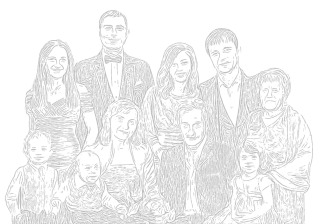
\includegraphics[width=\textwidth]{_cover/to.jpg}
    \emph{Dedicated to my Family}\\
  \end{minipage}
\end{figure}
~
\vspace{2cm}

\noindent The purpose of this book is not merely to instruct but to embark on a shared journey into the realm of 
platform-agnostic application development using Flutter. I've started that book by knowing nothing about Flutter and 
Dart, and the spent time have given me just an initial impulse to the mastery, but I still have something to share with 
you. 

\vspace{3mm}

\noindent I am confident that the time spent on coding (approximately 200 hours) can suffice for grasping the 
fundamental concepts of any programming language or framework, regardless of your prior background, as long as you 
progressively tackle more complex tasks while gradually reducing the need for assistance.

\vspace{3mm}

\noindent My approach to learning has evolved into a day-to-day habit, which I've diligently followed over the past 
20 years while working as a full-stack developer. My technical proficiency is complemented by a profound customer 
focus and business acumen. That possess insights into a product, project, and software life cycles.

\vspace{3mm}

\noindent I warmly invite you to join this project as it unfolds throughout the pages of this book. Together, we will 
embark on an exploration of Flutter and its extensive capabilities. This collaborative learning journey promises to 
be both exciting and enriching as we delve further into the depths of this versatile framework.


\vspace{1cm}

%\texttt{Contributors:}
%Viachaslau Lyskouski, ...

\noindent \emph{\small © Viachaslau Lyskouski, 2023: Creative Commons Attribution-NonCommercial-NoDerivatives 4.0 
International (CC BY-NC-ND 4.0)}
            

\newpage
\thispagestyle{empty}
~

\tableofcontents

%\listoffigures

%\listoftables

\newpage
\section*{Introduction}
\addcontentsline{toc}{section}{Introduction}
% Copyright 2023 The terCAD team. All rights reserved.
% Use of this content is governed by a CC BY-NC-ND 4.0 license that can be found in the LICENSE file.

Dear readers, I invite you to join me on a journey into a platform-agnostic application development, starting from 
ground zero. Meaning, that we (me and, possibly, you) might know nothing about cross-platform or mobile development, 
\q{Flutter}-framework, \q{Dart}-language, by not having even an idea for the application; ideally, it might 
be chosen a market, which to shake (in our case, -- financial accounting).

That book might be misaligned with the concepts that you're following, respecting, or adepting; by representing the 
author's vision, that's why I invite you to argue with me (\emph{and kindly request your assistance in identifying 
possible errors and misprints}) on the pages of a repository that contains the sources of this book and an application 
that we'll develop together as reading through 
\href{https://github.com/lyskouski/app-finance}{https://github.com/lyskouski/app-finance}. And... 
who knows, may be your arguments will change the ground ideas of that book, and we'll republish it together. 
So, here are those statements:

\begin{itemize}
\setlength{\itemsep}{3pt}
\setlength{\parskip}{0pt}
\setlength{\parsep}{0pt}
    \item Creating any program is similar to a pottery workshop flow, by taking amorphous idea and shaping it. Through 
    the time it can be changed an architectural style (homogeneous, layered, multitier, microservices, etc.), structure 
    (monolithic, distributed, hierarchical, etc.), even platform (from platform specific to serverless), and language. 
    It's all about being Agile, being adaptive to all external and internal challenges. Meaning, that the application's 
    revenue justifies any refactoring, including the possibility of re-creating it from scratch.

    \item Programming is not something about creativity, in its pragmatic meaning (\emph{no one, except the author, 
    will be able to accurately obtain the same result if the same initial situation is created}), but mastery 
    (\emph{how accurate, quick, balanced, and far-sighted will be your implementation}).

    \item Instruments (languages, frameworks, libraries, etc.) should be adapted to solve the problem instead of 
    adapting initial ideas to a capability of available / known tools.

    \item Instead of being \q{I}, \q{T}, \q{U}, or \q{M}-shaped, nowadays dictate us to be \q{\_}-shaped 
    (underscore-shaped). While the most scientists maintain a broad outlook with a narrow specialty (\q{T}-shaped), a 
    significant portion of programmers stand on an unstable foundation. Meaning that technologies are infinitely 
    replacing each other through the time via tick-tock model (characterized by periods of evolution and revolution) 
    and the most effective approach is to continuously expand one's fundamental knowledge (polymathy, \cite{Root09}) 
    by staying acquainted with the technologies in use. 
\end{itemize}

\noindent In case of having any discrepancies with this, the book may cause a rejection; and it's the best time to 
refund. Moreover, it is been started without any knowledge in mobile and cross-platform development, Flutter, Dart, and 
understanding the needs of "financial accounting" market. \q{ChartGPT} was used as a mentor, and \q{Midjourney} --
to generate a few images (including covers of that book), and "shared" some design insights.

Returning to the core themes of the book and the selected technologies, it's evident that businesses aim to embrace 
innovative technologies to optimize their processes and provide outstanding user experiences, all while ensuring 
broad platform compatibility. Not so far, Flutter (\emph{Dec 4th, 2018 -- version 1; May 10th, 2023 -- version 3}) 
has emerged as a popular choice for building high-performance, platform-agnostic (desktop, mobile, web) applications. 
And this book, "\emph{From Nothing to Market with Flutter: Desktop, Mobile, and Web Distribution}", road us to a 
comprehensive journey through the creation of a robust competitive application by using Flutter with 
\q{no-server}-basis (while \q{serverless} is mostly associated with cloud-based infrastructure).

The central objective of this book is to illustrate how to harness the extensive capabilities of Flutter to build a 
comprehensive and feature-rich application. Across the chapters, we will delve into every phase of the application 
development process, starting from conceptualization and culminating in distribution:

\begin{itemize}
    \item Take basics in \q{Dart}-language and \q{Flutter}-framework, and how it enables cross-platform development.

    \item Gain insights into the design principles of an application development. 
    
    \item Go through User Interface and Experience practices to create an intuitive user interface.

    \item Discover how to incorporate essential features into the application with a forecast release planning.

    \item Explore strategies for securely interacting with external systems and ensuring data integrity.

    \item Master techniques for testing (unit, widget, integration, and performance tests) and debugging practices. 

    \item Configure the application distribution across all platforms (Windows, Linux, MacOS, Android, iOS) to their 
    marketplaces, and explore strategies for ongoing maintenance and updates.
\end{itemize}

\noindent So, let's embark on this learning curve journey and keep \q{Flutter}ing.

\newpage
\section{[TBD] Bootcamping}
\input{./ch00-s01-dart}
Question: Flutter check that variable is a function

Answer: In Flutter, you can use the is operator to check if a variable is a function. 

\begin{lstlisting}
void main() {
  var variable = () {
    // Function body
  };

  if (variable is Function) {
    print('Variable is a function');
  } else {
    print('Variable is not a function');
  }
}
\end{lstlisting}

In this example, the is operator is used to check if the variable is of type Function. If it is, the condition 
variable is Function will evaluate to true, indicating that the variable is a function. Otherwise, it will 
evaluate to false, indicating that the variable is not a function.


Question: flutter default value in constructor

Answer: In Flutter, you can assign default values to constructor parameters using the = operator. 

\begin{lstlisting}
class MyClass {
  final int myValue;

  MyClass({this.myValue = 10});
}
\end{lstlisting}

In the example above, the MyClass constructor has a parameter myValue with a default value of 10. 
If no value is provided for myValue when creating an instance of MyClass, it will default to 10.

You can then create an instance of MyClass with or without providing a value for myValue:

\begin{lstlisting}
// Using the default value
MyClass instance1 = MyClass();
print(instance1.myValue); // Output: 10

// Providing a custom value
MyClass instance2 = MyClass(myValue: 20);
print(instance2.myValue); // Output: 20    
\end{lstlisting}

In the first case, where no value is provided for myValue, it takes on the default value of 10. In the second case, 
a custom value of 20 is provided, which overrides the default value.


Question: Operating with Dates
As an example, first business logic
if endDate <= currentDate then return 1
if startDate = currentDate then return 0
else return related float

\begin{lstlisting}
double calculateValue(DateTime startDate, DateTime endDate, DateTime currentDate) {
  if (endDate.isBefore(currentDate) || endDate.isAtSameMomentAs(currentDate)) {
    return 1.0;
  } else if (startDate.isAtSameMomentAs(currentDate)) {
    return 0.0;
  } else {
    double totalDays = endDate.difference(startDate).inDays.toDouble();
    double currentDays = currentDate.difference(startDate).inDays.toDouble();
    return currentDays / totalDays;
  }
}
\end{lstlisting}

In this example, the calculateValue function takes three DateTime parameters: startDate, endDate, and currentDate.

If endDate is less than or equal to currentDate, it means the end date has passed or is the same as 
the current date, so we return 1.0.
If startDate is the same as currentDate, we return 0.0.
Otherwise, we calculate the float value based on the ratio of the number of days between startDate and 
currentDate to the total number of days between startDate and endDate.

To get the current date in Flutter, you can use the DateTime class along with the DateTime.now() method. 
% Copyright 2023 The terCAD team. All rights reserved.
% Use of this content is governed by a CC BY-NC-ND 4.0 license that can be found in the LICENSE file.

\markboth{Bootcamping Flutter}{Bootcamping Flutter}

[TBD]


\subsubsection{Asserting Functions Definition}

By defining functions as arguments for widgets, we can use then as an expectation of functions structure.

\begin{lstlisting}
typedef SetViewFunction = String Function(Currency input);

class CurrencySelector extends StatelessWidget {
  SetViewFunction? setView;

  CurrencySelector({
    Key? key,
    this.setView,
  }) {
    setView ??= setDefaultView;
  }

  String setDefaultView(Currency input) {
    // Default implementation
  }
}
\end{lstlisting}


\subsubsection{Ignoring Function Arguments}

Not required fields are specified slightly different in comparison with classes constructors:

\begin{lstlisting}
void add(String value, [int? id]);
\end{lstlisting}


\subsubsection{Applying Getters and Setters for Class Variables}

By migrating our data structures to class objects it can be used additionally getter and setter for class variables.
That will help us to cover, as an example, \q{description}-attribute for Budget structures by showing 
"Spent Amount / Total Budget", and for \q{details}-attribute - "Left Amount".

\begin{lstlisting}
class MyClass {
  String _name; // Private variable

  // Getter for name
  String get name => _name;

  // Setter for name
  set name(String value) {
    _name = value;
  }
}

void main() {
  MyClass myObject = MyClass();

  // Using the setter
  myObject.name = 'John';

  // Using the getter
  print(myObject.name); // Output: John
}
\end{lstlisting}

In the example above, the \q{MyClass}-class has a private variable \q{\_name}. The getter for \q{\_name} is defined 
using the get keyword, and the setter is defined using the set keyword. The getter returns the value of 
\q{\_name}, and the setter sets the value of \q{\_name} to the provided value. By using that approach we can control 
the access to class variables and perform additional logic or validation when getting or setting their values.

One more question, is how to set \q{DateTime.now()} inside a constructor as default value, since, by defining it inside
the constructor, an error would be taken: The default value of an optional parameter must be constant.

So, to set a default value for a DateTime variable as the current date and time, we can use the \q{DateTime.now()} method 
during the initialization of the variable.

\begin{lstlisting}
class MyClass {
    DateTime _createdAt;

    MyClass({DateTime? createdAt})
        : _createdAt = createdAt ?? DateTime.now();

    DateTime get createdAt => _createdAt;
}
\end{lstlisting}


\subsubsection{Using cast to resolve dynamic structures}

Migration our Bills to classes construction has lead to an error on .firstWhere when Account of Budget not found. 
To resolve that we have to cast our getter (otherwise it would be an error: type '() => dynamic' is not a subtype 
of type '(() => BudgetAppData)?' of 'orElse') and add orElse operator as following:

\begin{lstlisting}
  dynamic getByUuid(AppDataType property, String uuid) {
    var scope = (_data[property] as Map)['list'];
    return scope.cast<dynamic>() // cast to cover different types, 
    .firstWhere(
      (item) => item.uuid == uuid,
      orElse: () => null, // Return null if not found
    );
  }
\end{lstlisting}


\subsubsection{Differentiating Map Types}

\q{HashMap}, as named, provides access to items by their hash in (potentially amortized) constant time.

\q{SplayTreeMap}' is based on a self-balancing binary tree that allows most single-entry operations in amortized 
logarithmic time.

\begin{lstlisting}
class SummaryAppData {
  // Tree provides improved state on sorting
  final _scope = SplayTreeMap<int, String>();
  // Hash gives us better performance to search by key
  final _hash = HashMap<String, int>();

  SummaryAppData({
    required List<String> list,
  }) {
    this.list = list; // Cover the original property by get/set
  }

  // Return list in reversed order
  List<String> get list => _scope.values.toList().reversed.toList();

  set list(List<String> list) {
    for (int i = 0; i < list.length; i++) {
      add(list[i], i + 1);
    }
  }

  add(String value, [int? id]) {
    // Checking that our UUIDs are unique across the list
    if (_hash.containsKey(value)) {
      _scope.remove(_hash[value]);
      _hash.remove(value);
    }
    // Used to sort the list based on last modification 
    int key = id ?? DateTime.now().millisecondsSinceEpoch;
    _scope[key] = value;
    _hash[value] = key;
  }
}
\end{lstlisting}
% Copyright 2023 The terCAD team. All rights reserved.
% Use of this content is governed by a CC BY-NC-ND 4.0 license that can be found in the LICENSE file.

\markboth{Bootcamping Flutter}{Bootcamping Flutter}

[TBD]


\subsubsection{Asserting Functions Definition}

By defining functions as arguments for widgets, we can use then as an expectation of functions structure.

\begin{lstlisting}
typedef SetViewFunction = String Function(Currency input);

class CurrencySelector extends StatelessWidget {
  SetViewFunction? setView;

  CurrencySelector({
    Key? key,
    this.setView,
  }) {
    setView ??= setDefaultView;
  }

  String setDefaultView(Currency input) {
    // Default implementation
  }
}
\end{lstlisting}


\subsubsection{Ignoring Function Arguments}

Not required fields are specified slightly different in comparison with classes constructors:

\begin{lstlisting}
void add(String value, [int? id]);
\end{lstlisting}


\subsubsection{Applying Getters and Setters for Class Variables}

By migrating our data structures to class objects it can be used additionally getter and setter for class variables.
That will help us to cover, as an example, \q{description}-attribute for Budget structures by showing 
"Spent Amount / Total Budget", and for \q{details}-attribute - "Left Amount".

\begin{lstlisting}
class MyClass {
  String _name; // Private variable

  // Getter for name
  String get name => _name;

  // Setter for name
  set name(String value) {
    _name = value;
  }
}

void main() {
  MyClass myObject = MyClass();

  // Using the setter
  myObject.name = 'John';

  // Using the getter
  print(myObject.name); // Output: John
}
\end{lstlisting}

In the example above, the \q{MyClass}-class has a private variable \q{\_name}. The getter for \q{\_name} is defined 
using the get keyword, and the setter is defined using the set keyword. The getter returns the value of 
\q{\_name}, and the setter sets the value of \q{\_name} to the provided value. By using that approach we can control 
the access to class variables and perform additional logic or validation when getting or setting their values.

One more question, is how to set \q{DateTime.now()} inside a constructor as default value, since, by defining it inside
the constructor, an error would be taken: The default value of an optional parameter must be constant.

So, to set a default value for a DateTime variable as the current date and time, we can use the \q{DateTime.now()} method 
during the initialization of the variable.

\begin{lstlisting}
class MyClass {
    DateTime _createdAt;

    MyClass({DateTime? createdAt})
        : _createdAt = createdAt ?? DateTime.now();

    DateTime get createdAt => _createdAt;
}
\end{lstlisting}


\subsubsection{Using cast to resolve dynamic structures}

Migration our Bills to classes construction has lead to an error on .firstWhere when Account of Budget not found. 
To resolve that we have to cast our getter (otherwise it would be an error: type '() => dynamic' is not a subtype 
of type '(() => BudgetAppData)?' of 'orElse') and add orElse operator as following:

\begin{lstlisting}
  dynamic getByUuid(AppDataType property, String uuid) {
    var scope = (_data[property] as Map)['list'];
    return scope.cast<dynamic>() // cast to cover different types, 
    .firstWhere(
      (item) => item.uuid == uuid,
      orElse: () => null, // Return null if not found
    );
  }
\end{lstlisting}


\subsubsection{Differentiating Map Types}

\q{HashMap}, as named, provides access to items by their hash in (potentially amortized) constant time.

\q{SplayTreeMap}' is based on a self-balancing binary tree that allows most single-entry operations in amortized 
logarithmic time.

\begin{lstlisting}
class SummaryAppData {
  // Tree provides improved state on sorting
  final _scope = SplayTreeMap<int, String>();
  // Hash gives us better performance to search by key
  final _hash = HashMap<String, int>();

  SummaryAppData({
    required List<String> list,
  }) {
    this.list = list; // Cover the original property by get/set
  }

  // Return list in reversed order
  List<String> get list => _scope.values.toList().reversed.toList();

  set list(List<String> list) {
    for (int i = 0; i < list.length; i++) {
      add(list[i], i + 1);
    }
  }

  add(String value, [int? id]) {
    // Checking that our UUIDs are unique across the list
    if (_hash.containsKey(value)) {
      _scope.remove(_hash[value]);
      _hash.remove(value);
    }
    // Used to sort the list based on last modification 
    int key = id ?? DateTime.now().millisecondsSinceEpoch;
    _scope[key] = value;
    _hash[value] = key;
  }
}
\end{lstlisting}

\newpage
\section{[TBD] Observing Serverless Computing}
% Copyright 2023 The terCAD team. All rights reserved.
% Use of this content is governed by a CC BY-NC-ND 4.0 license that can be found in the LICENSE file.

\markboth{Observing Serverless Computing}{Observing Serverless Computing}

[TBD]

\newpage
\section{[TBD] Conceptualizing Design}
% Copyright 2023 The terCAD team. All rights reserved.
% Use of this content is governed by a CC BY-NC-ND 4.0 license that can be found in the LICENSE file.

In the realm of transient concepts, many individuals tend to become perplexed. The truth is, nearly every idea we 
utilize is an amalgamation of numerous insights contributed by diverse individuals spanning a considerable span of 
time. Pioneering ideas entirely from the ground up often proves to be a futile endeavor. Instead, the optimal approach 
involves assimilating the finest aspects of what has already been established and then enhancing upon that foundation
(\cite{John11}, \cite{Azar22}, \cite{Page19}, \cite{Bara18}, \cite{Kleo12}, \cite{Thag12}).

There can be different strategies for the product creation \cite{Lomb17} but we're not going to concentrate on that,
and declare a Disruptive Product with an initial phase in three months (since it's a free-spot time allocation
for a single developer, me; approximately 200 hours). Disruptive strategy is stand out by providing a simple, 
cost-effective solutions to customers' challenges. 

For instance, when Netflix was introduced, it didn't immediately disrupt the market due to the lack of instant 
gratification for customers who were used to buying movies from Blockbuster stores. However, as Netflix 
improved its service, reducing movie delivery time and eventually introducing online streaming, it ultimately led 
to the downfall of Blockbuster stores \cite{Eby17}.

\paragraph{Project Assumption} In today's fast-paced world, managing personal finances has become increasingly 
important. Whether it's tracking expenses, setting budgets, or monitoring investments, individuals are seeking for an 
efficient and intuitive solution to keep their financial lives in order (take control of finances).


\subsection{Simplifying User Interface}
\markboth{Conceptualizing}{Simplifying User Interface}

One of the fundamental principle in designing an application is a simplicity. The application should have a clean and 
intuitive interface, allowing users to effortlessly navigate through various sections and perform tasks. We should avoid 
overwhelming users with unnecessary complexities and focus on providing a streamlined experience that caters to 
their specific needs. Since the main goal is to create the application that can be easily understood and used by a wide 
range of users, regardless of their level of technical expertise.

A \textbf{Minimalistic Design} philosophy guides this endeavor. By keeping the user interface uncluttered and avoiding 
excessive information or visual elements, the application becomes visually appealing and organized. White space, clear 
typography, and a consistent color scheme contribute to a visually pleasing and organized interface.
Furthermore, clear navigation is essential. The navigation within the application should be intuitive and 
straightforward. This involves using descriptive labels for navigation elements like tabs, menus, and buttons. 
The logical organization of different sections and features ensures that users can find what they need without 
confusion or frustration. By maintaining the consistent placement of buttons, menus, and interactive elements, users 
can develop a mental model of the application interface. This allows them to predict how different actions and 
interactions will unfold based on their previous experiences within the app.

\textbf{Task-Oriented Design} (TOD) places specific tasks and goals at the forefront. The application is designed 
around these tasks, providing clear and easily accessible options for the most commonly performed scenarios.
For instance, when it comes to Smart Speakers, we shift from a Graphical User Interface (GUI) to a Voice User Interface 
(VUI). The overarching objective of Task-Oriented Design is to create a solution that maintains a cohesive product 
identity across various platforms while tailoring features to suit the specific capabilities of each device type.
Within the framework of Task-Oriented Design, the application seamlessly integrates contextual assistance and guidance. 
This encompasses the deployment of tooltips, on-screen cues, and informative messages, strategically delivering 
pertinent information precisely when it is needed. Efficient data entry is facilitated through a range of 
functionalities, including auto-suggestions, pre-filled forms coupled with input assistance validation, and 
intelligent categorization through the application of smart defaults. Where as an application feedback reassures users 
that their inputs have been successfully registered and processed. This adds to the overall user confidence in the 
application.

By observing how users interact with the application and identifying pain points, the design can be refined based on 
their input. The iterative approach allows for addressing usability issues and continually enhancing the user 
experience. So, the user testing and iteration further refine the application, ultimately creating an interface that 
caters to a diverse user base.

Last but not least, the application should be accessible to users with disabilities, by following \textbf{Accessibility 
Guidelines and Standards}. This ensures that individuals with visual impairments, motor limitations, or other 
accessibility needs can use the application. Options for adjusting font sizes, color contrasts, and support for 
screen readers are essential elements of this inclusivity. It's worth noting that approximately 15\% of the global 
population faces some form of disability, and regrettably, over 80\% of websites and applications fall short in 
addressing their needs \cite{Worl11}. While achieving the full compliance might be challenging (\emph{targeted 
automated testing frameworks can catch less than 25\% of accessibility issues}, \cite{Univ22}), adherence to these 
principles remains of paramount importance.

\img{concept/apple-calendar}{Task-Oriented Design -- Apple Calendar \cite{Thal20}}{img:fs-calendar}

\subsection{Hierarching Information}
\markboth{Conceptualizing}{Hierarching Information}

A well-designed financial accounting application must establish a clear information hierarchy. It's imperative to place 
critical financial data, such as account balances, transactions, and budgets, front and center, ensuring that users can 
access these key details with ease. That reduces a cognitive load by making it easier to understand the status and make 
informed decisions.

To construct the information effectively we need to identify the most crucial data that users should readily see and 
rely on, and prominently display it on the application's main screen. By keeping things organized and user-friendly, 
we should categorize and group data logically. This involves utilizing clear headings and visual cues to differentiate 
between various categories, making data retrieval a breeze. So, let's harnesses the power of a \textbf{Visual Hierarchy}. 
It guides users' attention to important details by employing tactics such as larger fonts, contrasting colors, and 
meticulous typography. 

Utilization of a \textbf{Progressive Disclosure} is started from offering users a high-level overview, with the 
flexibility to delve deeper for more detailed information by using intuitive gestures and interactions. This approach 
ensures that users can access the level of detail that aligns with their needs without being overwhelmed by complexity. 
This is achieved by maintaining a consistent layout and organizational structure across different screens and sections 
of the application without relearning the interface. Our objective is to streamline data entry, minimize user effort, 
and enhance user understanding. By offering the contextual information and explanations where needed, we aid users in 
understanding the significance of different terms or calculations, complex concepts or unfamiliar jargon. We ensure 
that labels accurately represent the actions or functions they perform and complement these labels with appropriate 
icons for quick recognition and comprehension. This entire user-friendly interface is made complete by its adaptability 
to various screen sizes and orientations that users may employ.


\subsection{Onboarding}
\markboth{Conceptualizing}{Onboarding}

The onboarding process in a financial accounting application is a critical step in ensuring user engagement and 
long-term retention. Its primary goal is to guide users through the initial setup and familiarize them with the 
key features of the application. A well-designed onboarding process boosts user confidence, minimizes friction, and 
lays the foundation for lasting engagement and satisfaction.

The journey begins with a concise yet compelling introduction, clearly outlining the application's value proposition 
and highlighting its distinctive features. This initial introduction is crucial in setting the stage for what users 
can expect. Following the introduction, a guided setup process is introduced. This process is thoughtfully divided 
into manageable stages, with each step presented one at a time. Explanatory text and visual cues accompany each step, 
ensuring users can easily navigate through the setup process. Each onboarding step is complemented by clear 
calls-to-action, providing users with explicit instructions on what they need to do next. These intuitive prompts 
make it simple for users to complete each task. Progress indicators are thoughtfully integrated to help users track 
their progress through the onboarding process. These visual cues reassure users that they're making headway and help 
manage their expectations regarding the remaining steps. The motivation and engagement are boosted through quick wins 
and rewards, fostering a positive user experience that encourages users to continue using the application.

As the onboarding process concludes, users are invited to provide feedback. This open channel for user input, questions, 
and issue reporting is invaluable for identifying areas of improvement and enhancing the evolving onboarding experience.

By incorporating all of these elements into the onboarding process, the application aims to enhance user understanding, 
satisfaction, and long-term engagement, setting the stage for a successful and user-friendly experience.


\subsection{Personalizing Options}
\markboth{Conceptualizing}{Personalizing Options}

Empowering users to tailor the application to their unique requirements, needs, and preferences is at the heart of 
personalization options. One aspect of this personalization involves accommodating diverse users by providing support 
for multiple languages (and currencies). This ensures that users feel comfortable (a data interpretation) and fosters 
a sense of ownership.

Customization extends to categories, allowing users to create and personalize data sections. These tags help improve 
data accuracy and relevance. Users can define budget limits for specific categories, restating frequencies like monthly 
or weekly to allocate funds effectively. The convenience of backing up their data and syncing it across multiple 
devices adds a further layer of personalization. Moreover, users can benefit from the ability to export their data in 
various formats and create customizable report templates.

Customizable \textbf{Dashboards} offer the flexibility to select the main page's content. Users can choose what 
information and widgets they want to see at a glance, arranging them according to their priorities. The ability to 
choose from various color schemes, fonts, and layouts further enhances the tailored experience. Customization in the 
application goes beyond layout changes. It extends to notifications, allowing users to personalize their experience 
by setting preferences for progress tracking, reminders, and insights. These tailored notifications are designed to 
keep users motivated and on track toward achieving their unique financial goals. Whether it's saving for a dream 
vacation, paying off debt, or planning for retirement, users can define their aspirations. The beauty of this feature 
lies in the granular control it provides over notification preferences, ensuring users stay informed without being 
overwhelmed, making their financial journey both effective and personalized.


\subsection{Securing Information}
\markboth{Conceptualizing}{Securing Information}

Securing financial data is a top priority in the design of any application. We should understand the sensitive nature 
of the information users entrust us with and are committed to ensuring its safety. Financial data is highly sensitive, 
and users need the assurance that their information is secure (such as the usage of end-to-end encryption and 
two-factor authentication). By prioritizing secure data handling practices, we may establish trust with users, mitigate 
risks, and safeguard a sensitive information. That can be made even more transparent and trustful by a regular security 
audits. These audits help us identify vulnerabilities and weaknesses in our application's infrastructure and codebase. 
That helps us to guarantee prompt correction of any known (identified) vulnerabilities.

Our application should employ robust \textbf{encryption} techniques to protect user data both in transit and at rest. 
This means that sensitive information, like account credentials, transaction details, and personal identifiers, is 
encrypted using industry-standard algorithms. Encryption adds an extra layer of protection and ensures that even if 
data is compromised, it remains unintelligible to unauthorized parties.

\textbf{Multi-Factor Authentication} (MFA) adds another level of confidence to user identity verification by requiring
a combination of something the user knows (a password), something they have (like a token or mobile device), or 
something they are (biometrics). With these stringent authentication procedures, users can trust that their accounts 
are well-protected. 

By implementing \textbf{Role-Based Access Control} (RBAC), we can precisely restrict access to sensitive data and critical 
functionalities according to predefined permissions. This ensures that only authorized personnel can interact with 
specific parts of the application, enhancing security and data protection. That allows us to meticulously manage access 
permissions by assigning roles to individuals. With that we have to establish robust secure storage mechanisms to 
safeguard user data, as data backups to mitigate the risks in scenarios such as system failures.

Finally, \textbf{Privacy Policy} should be transparent and explained in details to users the information about the 
types of data we collect, its purpose, and who can access it. We maintain transparency in how we secure user information 
and respond to security incidents, with user-friendly channels for reporting concerns. This commitment ensures that 
users are well-informed about their data and can trust our unwavering dedication to data security. User consent is an 
essential aspect of our data handling process, and we should be explicit about how user information is safeguarded and 
our protocols for addressing security incidents, providing easily accessible channels for users to voice any concerns. 
So, the transparency is essential in conveying how the user information is protected and security incidents are managed.


\subsection{Visualizing Data}
\markboth{Conceptualizing}{Visualizing Data}

A visual representation of data empower users to grasp information more effectively and gain better control over their 
financial situation.

We should start from creating a captivating overview \textbf{Dashboard} that provides a high-level summary of the 
information through charts, graphs, and key performance indicators (KPIs). These visuals illustrate essential data, 
such as account balances, income versus expenses, savings progress, or net worth.  By incorporating interactive features 
as zooming, panning, and filtering, we enable users to explore data in-depth. Visual indicators, such as progress bars 
and thermometers, are valuable tools for tracking progress toward goals and budget adherence. 

Metrics help to effectively compare different financial metrics or periods using side-by-side visualizations like bar 
charts, line graphs, or stacked area charts. With that users gain clarity on their spending habits, stay within 
their financial targets, and quickly identify areas of focus or anomalies within their data.


\subsection{Integrating Services}
\markboth{Conceptualizing}{Integrating Services}

To provide users with a comprehensive financial tracking experience, the application can be integrated with financial 
institutions and services. This integration enables users to seamlessly connect their bank accounts, credit cards, and 
investment platforms, facilitating the automatic import of transaction data. Synchronization features ensure real-time 
updates and effortless reconciliation between the application and external financial sources. By implementing secure 
industry-standard protocols like Open Banking APIs, the application establishes a reliable and secure connection with 
financial institutions. Regular updates of account balances and transaction information provide users with real-time 
visibility into their financial standing, supporting various account types, from checking and savings accounts to 
credit cards and investment accounts. 

Stringent data security measures, including encryption and secure data transmission, along with compliance with data 
protection regulations such as GDPR or CCPA, ensure user data remains safe. Whereas a robust error handling mechanism 
addresses connectivity issues, promptly notifying users of any encountered problems and offering clear instructions for 
resolution. 

Users should be able to transactions as verified or reconciled once cross-checked with their official bank statements, 
enhancing data accuracy and aiding in the identification of discrepancies or missing transactions. This comprehensive 
integration sets the stage for a holistic and effective financial tracking experience.


\subsection{Shaking the Market}
\markboth{Conceptualizing}{Shaking the Market}

The application has a potential to stand out in the market by identifying areas where users can reduce costs, 
providing valuable recommendations, and highlighting opportunities for optimizing their budgets. This capability 
sets it apart by actively assisting users in managing their finances more efficiently.

For instance, the Automated Expense Categorization feature streamlines the categorization process by automatically 
assigning categories like groceries, transportation, entertainment, bills, and more, based on transaction data. This 
eliminates the need for manual categorization, saving users significant time and effort and ensuring accurate expense 
tracking.

Real-time Expense Insights provide users with a comprehensive view of their spending patterns through visualizations, 
charts, and graphs. These tools highlight monthly spending trends, category breakdowns, and comparisons with previous 
periods. Incorporating forecasting and predictive analytics into these visualizations assists users in planning and 
decision-making. Trend lines project future income, expenses, or savings based on historical data, allowing users to 
anticipate future financial scenarios and make informed choices.

The \textbf{Intelligent Notifications} feature harnesses the power of artificial intelligence (AI) to offer users a 
personalized and proactive financial management experience. It identifies anomalies, like unexpected high expenses, 
and can even detect irregularities that might indicate potential issues, such as unauthorized charges. AI should offer 
actionable financial insights by suggesting adjustments (potential cost-cutting measures) to users' budget based on 
their spending patterns.


Furthermore, the application with employed \textbf{Optical Character Recognition} (OCR) technology may extract data 
from receipts. This means that users can simply take a photo of a receipt, and the application will automatically 
extract key information, making expense tracking even more user-friendly and efficient.


\subsection{Enhancing Continually}
\markboth{Conceptualizing}{Enhancing Continually}

Encouraging a culture of continuous improvement is vital to maintaining user loyalty and satisfaction. Actively seek 
feedback from users to identify areas for enhancement and regularly update the application to improve the overall user 
experience. User feedback serves as a valuable source of insights for enhancing functionality, usability, and the 
application's overall user experience. This iterative approach ensures that the application evolves and remains 
pertinent in a dynamically changing landscape, ultimately leading to increased user satisfaction and loyalty.

Diverse channels are provided for users to share their feedback, suggestions, and concerns, including in-app feedback 
forms, email support, community forums, or social media channels. Users can easily voice their opinions and are 
actively encouraged to provide feedback on their experience with the application, and even upvote others' ideas in a 
feature request system. That can be improved by periodic surveys and questionnaires are conducted to gather insights 
from users, specifically focusing on their satisfaction level, pain points, desired features, and overall user 
experience. This feedback is instrumental in identifying areas for improvement and prioritizing development efforts 
based on user needs and preferences.

Analytics tools might help to track a user behavior within the application, monitoring their navigation through 
different screens, identifying drop-off points, and tracking usage patterns. On the other hand, \textbf{Usability 
Studies}, which encompass a diverse group of users, provide valuable insights. These studies enable the observation of 
user interactions with the application, gather feedback on specific features or workflows, and are instrumental in 
pinpointing areas where users may encounter challenges or confusion. Together, these approaches create a comprehensive 
understanding of the user experience, helping to shape continuous improvements in the application. Also, it might be 
engaged enthusiastic users to gather feedback on upcoming features or major updates. Beta testers provide valuable 
insights, uncover edge cases, and help identify issues before a wider release.

A seamless bug reporting process is an essential component of any application. Reported issues should be promptly 
acknowledged, and transparent communication should be upheld throughout the resolution process. This commitment to 
user feedback and continuous improvement ensures the development of a dynamic and \textbf{User-Centric Application}, 
placing users at the core of the improvement journey. In addition, release notes or in-app notifications serve as clear 
channels for communicating updates, enhancements, and bug fixes, further demonstrating the commitment to actively 
listening to users.\\
\\

\noindent In the end, our mission is clear: create a financial accounting application that is intuitive, efficient, 
and inclusive. Through thoughtful design and unwavering attention to detail, we're shaping an experience that empowers 
users to effortlessly manage their finances while ensuring that no one is left behind.


\newpage
\section{[WIP] Prototyping}
% Copyright 2023 The terCAD team. All rights reserved.
% Use of this content is governed by a CC BY-NC-ND 4.0 license that can be found in the LICENSE file.

\subsection{Configuring Development Environment}
\markboth{Implementing Core Functionality}{Configuring Development Environment}

Assume, our first steps we're doing from knowing nothing neither about Flutter, nor Dart. So, the better way to start 
from that position is to use some templates (and Flutter kindly provides us such an option).

But, initially, we do need to download and install Flutter (\href{https://flutter.dev}{https://flutter.dev}) by 
following the installation instructions specific to operating system that is used (as an example, for Windows it 
would be needed to register library directory location in the system's \q{PATH}-variable after downloading its sources, 
\cref{img:fs-windows-path}).

\img{first-steps/windows-path-variable}{Windows 10 \q{PATH}-variable location}{img:fs-windows-path}

The choice of a better Integrated Development Environment (IDE) for Flutter development is something negligible, widely
proposed Visual Studio Code, Android Studio, IntelliJ IDEA; but the truth is that nobody cares, what was used (even VIM,
Notepad, or nano), if the work is done. Nonetheless, further discussions in the book would be relevant to Visual 
Studio Code (\href{https://code.visualstudio.com/}{https://code.visualstudio.com/}) usage in "how-to configure IDE" 
examples if nobody minds.

With Visual Studio Code, let's start from Extensions Marketplace usage by installing "Flutter" and "Dart" extensions, 
right after that IDE will ask regarding the Flutter Software Development Kit (SDK) folder (it's the directory where 
the Flutter was installed / downloaded into).

Inside the Flutter SDK folder, we may find a various directories and files, including:

\begin{itemize}
  \item bin -- Flutter command-line tools, such as \q{flutter}, \q{dart}, and other utilities;
  \item cache -- cached files and downloaded packages;
  \item doc -- documentation;
  \item examples -- code examples and sample projects;
  \item packages -- core Flutter packages and dependencies.
\end{itemize}

After those steps, in Visual Studio Code from Command Palette (by pressing [Ctrl + Shift + P], or [Cmd + Shift + P] 
on macOS) will become available "Flutter: New Project"-command, by clicking on which prompt will ask regarding project 
name and location to generate a basic structure. Going farther, let's open the project in IDE and frustrate a minute 
about a wide variety of different scaring files that's been generated. Breathe... we do need only one of them by 
now, that's located in the \q{lib}-directory. File \q{main.dart} is the project's central orbit, the entry point of our 
application.

\begin{lstlisting}
// ./lib/main.dart
import 'package:flutter/material.dart';
// Entry point
void main() {
  runApp(const MyApp());
}
// 'Stateless' means missing any saved states of MyApp
class MyApp extends StatelessWidget {
  // 'super' - parent class, 'key' - widget unique identifier
  const MyApp({super.key}); // Class constructor
  
  // '@override' - replace implementation from parent class
  @override
  Widget build(BuildContext context) { // Returns 'Widget' instance
    return MaterialApp(
      title: 'Flutter Demo',
      // Application theme definition
      theme: ThemeData(
        // Basic color scheme
        colorScheme: ColorScheme.fromSeed(seedColor: Colors.deepPurple),
        // Configuration of Widgets' styles
        useMaterial3: true,
      ),
      // Main page definition
      home: const MyHomePage(title: 'Flutter Demo Home Page'),
    );
  }
}
// 'Stateful' to re-render widget by changed internal states
class MyHomePage extends StatefulWidget {
  // 'required' means that 'title' is a mandatory for constructor on line 25
  const MyHomePage({super.key, required this.title});
  // 'final' - cannot be changed afterwards
  final String title;
  // Wrap an object for a state management
  @override
  _MyHomePageState createState() => _MyHomePageState();
}
// Underscore is a convention for internal classes, methods, and variables
class _MyHomePageState extends State<MyHomePage> {
  int _counter = 0;
  // Internal method to update '_counter' state
  void _incrementCounter() {
    // 'setState' - a special method to save state
    // ... and re-trigger 'build'-method
    setState(() {
      _counter++;
    });
  }
  // Mandatory method for any Widget-based classes
  @override
  Widget build(BuildContext context) {
    return Scaffold(
      appBar: AppBar(
        backgroundColor: Theme.of(context).colorScheme.inversePrimary,
        title: Text(widget.title),
      ),
      body: Center(
        child: Column(
          mainAxisAlignment: MainAxisAlignment.center,
          children: <Widget>[
            // Usage of 'const' is recommended to improve performance
            // ... for any Widget that's not having a dynamic parameters
            const Text(
                'You have pushed the button this many times:',
            ),
            Text(
              '$_counter', // '$' - for a variable interpolation
              style: Theme.of(context).textTheme.headlineMedium,
            ),
          ],
        ),
      ),
      floatingActionButton: FloatingActionButton(
        onPressed: _incrementCounter,
        tooltip: 'Increment',
        child: const Icon(Icons.add),
      ),
    );
  }
}
\end{lstlisting}

Let's see results of a compilation (\cref{img:fs-app}) by triggering \q{flutter run}-command from a terminal of the 
project directory (as an example, for Visual Studio Code by clicking on "View" in the top menu, selecting "Terminal"; 
short key [Ctrl + backtick]). If no emulators are enabled, it may ask to clarify the type of execution.

\img{first-steps/app-template}{First run with autogenerated application}{img:fs-app}

Valuable tip for any development process is to activate a debug mode, that can be done simply by adding \q{--debug} to 
the previous console command (sample, \q{flutter run -d windows --debug} to run project on Windows in debug mode). Then, 
the process is similar to any other programming language: set breakpoints in a code by clicking in IDE on the left 
margin of the desired line, use the command, inspect variables and their states by stepping through the code. Instead of
any debug mode it can be simply used \q{print}-function to plot anything into console. By taking into account that we 
might know exactly nothing about Flutter (and, possibly, any other programming languages), let's return to that 
statement when our application (and we) will become more mature... too early without any business logic on board.

What we can do in addition, is to emulate a real device usage. That's achievable with the Android SDK by downloading 
(\href{https://developer.android.com/studio}{https://developer.android.com/studio}), installing, and going through 
the initial wizard setup (nothing special by now, choose everything by default). One additional step is to create a 
virtual device (\cref{img:fs-android})... a couple of clicks and we're done (\cref{img:fs-create}).

Once we've set up Android SDK and triggered "Start" for the emulator, Flutter will recognize its availability from
an execution \q{flutter run}. Flutter app will be build and launched on the connected Android emulator (or even real 
device, connected via USB; check manuals if needed).\\

\img{first-steps/android-studio}{Android Studio start page}{img:fs-android}
\img{first-steps/android-studio-create}{Android Studio choose and create Emuator}{img:fs-create}

\noindent Let's dive into the coding!
% Copyright 2023 The terCAD team. All rights reserved.
% Use of this content is governed by a CC BY-NC-ND 4.0 license that can be found in the LICENSE file.

\subsection{Unlocking Multi-Platform}
\markboth{Prototyping}{Unlocking Multi-Platform}

Flutter is designed to work seamlessly across all environments. However, there are a certain scenarios, such as file
handling, where its behavior may deviate from being entirely platform-agnostic. Independently of that, there are two
ways to brake that limitation.\\
\\

\noindent Conditional imports:

\begin{lstlisting}
import 'package:file_picker_web/file_picker_web.dart' if (dart.library.io) 'package:file_picker/file_picker.dart';
\end{lstlisting}

\noindent and exports:

\begin{lstlisting}
export 'src/connector_none.dart' // Stub implementation
  if (dart.library.io) 'src/connector_io.dart' // dart:io
  if (dart.library.html) 'src/connector_html.dart'; // dart:html
\end{lstlisting}

% Copyright 2023 The terCAD team. All rights reserved.
% Use of this content is governed by a CC BY-NC-ND 4.0 license that can be found in the LICENSE file.

\subsection{[TBD] Prototyping Application Skeleton}
\markboth{Implementing Core Functionality}{Prototyping Application Skeleton}

[TBD]

\subsubsection{Creating Widget Tests} \label{widget-tests}

By now we've created some business logic functionality with not so trivial flow. Not to waste the time on checking it
all the time manually after significant changes or refactoring, let's create some tests to check it for us automatically.

Furthermore we've already broken our first test (that's been provided by a Flutter template generation). At the 
beginning it was covering the `Add`-button as an incremental trigger for the shown counter.

\begin{lstlisting}
void main() {
  testWidgets('Counter increments smoke test', (WidgetTester tester) async {
    // Build our app and trigger a frame.
    await tester.pumpWidget(const MyApp());

    // Verify that our counter starts at 0.
    expect(find.text('0'), findsOneWidget);
    expect(find.text('1'), findsNothing);

    // Tap the '+' icon and trigger a frame.
    await tester.tap(find.byIcon(Icons.add));
    await tester.pump();

    // Verify that our counter has incremented.
    expect(find.text('0'), findsNothing);
    expect(find.text('1'), findsOneWidget);
  });
}
\end{lstlisting}

\noindent Let's check that `Add`-button is opening a Widget with a three named tabs.

\begin{lstlisting}
void main() {
  testWidgets('Given Main page When tap on Create Then opened BillAddPage', (WidgetTester tester) async {
    // App initialization
    await tester.pumpWidget(
        // Taken as is from `void main` of `lib/main.dart`-file
        ChangeNotifierProvider(
            create: (_) => AppData(),
            child: const MyApp(),
        )
    );
    // Checking one of the text widgets
    expect(find.text('Goals'), findsOneWidget);
    // Clicking on `Add`-button
    await tester.tap(find.byIcon(Icons.add));
    await tester.pumpAndSettle(); // Waiting till finished render state
    // Asserting icons on our tabs
    expect(find.byIcon(Icons.insert_invitation), findsOneWidget);
    expect(find.byIcon(Icons.money_off), findsOneWidget);
    expect(find.byIcon(Icons.transform), findsOneWidget);
  });
}
\end{lstlisting}

Here we are, by `tab` and `expect` the flow of the whole application can be checked. Such type of tests are named as 
Widget tests that emphasized by specially named `testWidgets`-function.

Initially, it would be better to concentrate mostly on Business Logic than on the draft state of our pages. We'll 
return later to UI/UX, redesign if not dramatically but vastly, and right after that write a reliable 
Test Suite for the Widgets. To check business based calculations it's used `test`-function, and, by example, we would
take our implemented Account Recalculation flow.

\begin{lstlisting}
// test/unit/_classes/data/account_recalculation_test.dart 
void main() {
  // `group` works as a prefix to all the tests inside
  group('Account Recalculation:getDelta', () {
    late AccountRecalculation mock; // Deferred initialization 
    // `setUp` - is going to be executed before each test
    // `setUpAll` - once at the beginning of group evaluation
    setUp(() {
      final accountMock = AccountAppData(
        uuid: '1',
        title: 'test',
        type: AppAccountType.account.toString(),
      );
      mock = AccountRecalculation(
        initial: accountMock.clone(),
        change: accountMock.clone(),
      );
    });
    // Define "table" of input arguments and output assertions
    final testCases = [
      // initial  |   change   | result
      [false, 5.0,  false, 1.0,  -4.0],
      [false, 1.0,  false, 5.0,   4.0],
      [true,  2.0,  false, 3.0,   3.0],
      [false, 2.0,  true,  3.0,  -2.0],
    ];
    // Run all defined Test Cases
    for (var v in testCases) {
      test('initial(hidden[${v[0]}], details[${v[1]}]), change(hidden[${v[2]}], details[${v[3]}]) => ${v[4]}', () {
        // Update inputs
        mock.initial!.hidden = v[0] as bool;
        mock.initial!.details = v[1] as double;
        mock.change.hidden = v[2] as bool;
        mock.change.details = v[3] as double;
        // Assert `AccountRecalculation.getDelta`-method results
        expect(mock.getDelta(), v[4]); 
      });
    }
  });
}
\end{lstlisting}

By typing `flutter test` in the command line we would see something like that:

\begin{lstlisting}
[V] Given Main page When tap on Create Then opened BillAddPage
[V] Account Recalculation:getDelta initial(hidden[false], details[5.0]), change(hidden[false], details[1.0]) => -4.0
[V] Account Recalculation:getDelta initial(hidden[false], details[1.0]), change(hidden[false], details[5.0]) => 4.0
Expected: <3.0>
  Actual: <1.0>
[X] Account Recalculation:getDelta initial(hidden[true], details[2.0]), change(hidden[false], details[3.0]) => 3.0
[V] Account Recalculation:getDelta initial(hidden[false], details[2.0]), change(hidden[true], details[3.0]) => -2.0
Null check operator used on a null value
[X] Account Recalculation:getDelta initial(null), change(hidden[false], details[2.0]) => 2.0
Exited (1)
\end{lstlisting}

\noindent That test has highlighted a dozen of troubles and failures in our code, so, it definitely has not been 
written in vain.

\begin{lstlisting}[firstnumber=17]
// ./lib/_classes/data/account_recalculation.dart
double getDelta() {
  return change.hidden
\end{lstlisting}
{
\xpretocmd{\lstlisting}{\vspace{-12pt}}{}{}
\begin{lstlisting}[firstnumber=20, backgroundcolor=\color{backred}]
(*@\kdiff{-}@*)  ? -initial!.details
\end{lstlisting}
\begin{lstlisting}[firstnumber=20, backgroundcolor=\color{backgreen}]
(*@\kdiff{+}@*)  ? -(initial?.details ?? 0.0)
\end{lstlisting}
\begin{lstlisting}[firstnumber=21, backgroundcolor=\color{backred}]
(*@\kdiff{-}@*)  : change.details - initial!.details;
\end{lstlisting}
\begin{lstlisting}[firstnumber=21, backgroundcolor=\color{backgreen}]
(*@\kdiff{+}@*)  : (initial?.hidden ?? true
(*@\kdiff{+}@*)      ? change.details
(*@\kdiff{+}@*)      : change.details - initial?.details);
\end{lstlisting}
\begin{lstlisting}[firstnumber=24]
}
\end{lstlisting}
}

\subsubsection{Creating Automated Quality Gates}

Tests writing is not enough for a quality check, we have to implement some dozen of automation till the phase 
when will become too lazy to trigger that manually. In addition, Flutter provides a couple of commands for the 
code improvement:
\begin{lstlisting}
flutter analyze // Static analysis of Dart code
dart format // Apply rules from https://dart.dev/effective-dart/style#formatting
dart fix // Check what can be improved, by `--apply` will change the code
\end{lstlisting}


\paragraph{Creating Git Hooks}

Someone might think that additional checks before `git commit` and `git push` will slowdown the development process, 
contrary that minimizes pushes back and forward to resolve failures on CI/CD build procedure. For a really big projects
that might take hours in contrast with seconds on local environment. Surely, the automation process has to be done
accurately and properly, otherwise it will be constantly bored.

Implementing git hooks is a preparation of bash-scripts for execution, so, let's discuss here `pre-push`-file (since
`pre-commit`-file contains almost the same logic for another scope of commands).

\begin{lstlisting}[language=bash]
#!/bin/bash

status=0

flutter test # Trigger tests
status_test=$? # Take status for lastly executed command

if [ $status_test -ne 0 ]; then
  echo "[x] flutter test - failed."
  status=1
else
  echo "[+] flutter test - passed."
fi

exit $status
\end{lstlisting}

\noindent Let's use Grinder to install our hooks (`dart run grinder:init` can be used to generate a skeleton 
structure if it's missing yet).

\begin{lstlisting}
// ./tool/grind.dart
import 'dart:io';
import 'package:path/path.dart' as path;
import 'package:grinder/grinder.dart';

main(args) => grind(args);

@Task('Install Git Hooks')
installGitHooks() {
  final currDir = Directory('./');
  final hookDir = Directory('./.git/hooks');
  final hookNames = ['pre-commit', 'pre-push'];
  for (final name in hookNames) {
    log('Applying: $name');
    final sourceFile = File(path.join(currDir.absolute.path, name));
    sourceFile.copySync(path.join(hookDir.absolute.path, name));
  }
  log('Git Hooks applied!');
}
\end{lstlisting}

\noindent After that by using command line, let's check what we have:

\begin{lstlisting}[language=bash]
$ dart run grinder -h
Dart workflows, automated.

Usage: grinder [options] [<tasks>...]

Global options:
  --no-color           Whether to use terminal colors.
  --version            Reports the version of this tool.
  -h, --help           Print this usage information.

Available tasks:
  install-git-hooks    Install Git Hooks
  sort-translations    Update Translations by sorting values alphabetically

$ dart run grinder install-git-hooks
  grinder running install-git-hooks
  
  install-git-hooks
    Applying: pre-commit
    Applying: pre-push
    Git Hooks applied!
  
  finished in 0.0 seconds

$ git add .
$ git commit -m "Sample Commit"
Computing fixes in app-finance (dry run)...
Nothing to fix!
Formatted 56 files (0 changed) in 0.42 seconds.

[+] dart fix - passed.
[+] dart format - passed.
[+] dart run grinder sort-translations - passed.
Sample Commit
 3 files changed, 65 insertions(+), 90 deletions(-)

$ git push
# ... logs from tests
[+] flutter test - passed.
# ... other logs from git
\end{lstlisting}


\paragraph{Adding Grinder Helpers}

We haven't yet discussed our `grinder sort-translations` that was shown through the logs above. That task is needed
to automatically rearrange our labels in `/lib/l10n/app\_*.arb`-files. We might extend our grinder tasks lately
by also checking consistency (enter missing labels across the `.arb`-files), exporting labels to `.scv`-file
for translation purposes, and importing them back.

\begin{lstlisting}
// ./tool/grind.dart
import './localization.dart' as locale;

@Task('Update Translations by sorting values alphabetically')
sortTranslations() {
  // Get all additional arguments for the command
  TaskArgs args = context.invocation.arguments;
  // Run: dart run grinder sort-translations --quiet
  bool isQuiet = args.getFlag('quiet'); // Returns `true` if set
  bool isChanged = locale.sortArbKeys('./lib/l10n');
  if (isChanged && !isQuiet) {
    fail('Changes detected'); // (!) to handle failure
  }
}
\end{lstlisting}

\begin{lstlisting}
// ./tool/localization.dart
import 'dart:convert';
import 'dart:io';
import 'package:grinder/grinder.dart';

bool sortArbKeys(String path) {
  log('Checking $path'); // Add to console output the text
  final arbDir = Directory(path);
  bool isChanged = false;
  // Check, that folder is not missing
  if (!arbDir.existsSync()) {
    log('Error: Directory not found');
    return true;
  }
  // Loop per each file there
  for (var file in arbDir.listSync()) {
    // Take only .arb-files
    if (file is File && file.path.endsWith('.arb')) {
      log('- ${file.path}');
      // `|=` is a boolean OR assignment
      isChanged |= sortArbFileKeys(file);
    }
  }
  log(isChanged ? 'Labels reordered' : 'Nothing was changed');
  return isChanged;
}

bool sortArbFileKeys(File file) {
  // Load data from file
  final jsonContent = file.readAsStringSync();
  final arbMap = json.decode(jsonContent) as Map<String, dynamic>;
  // Sort labels
  final entries = arbMap.entries.toList();
  entries.sort((a, b) {
    final aKey = a.key.startsWith('@') ? a.key.substring(1) : a.key;
    final bKey = b.key.startsWith('@') ? b.key.substring(1) : b.key;
    return aKey.compareTo(bKey);
  });
  final sortedArbMap = Map.fromEntries(entries);
  // Write back to the file with preserved indentation
  const encoder = JsonEncoder.withIndent('    ');
  var jsonOutputContent = encoder.convert(sortedArbMap);
  file.writeAsStringSync(jsonOutputContent);
  return jsonOutputContent != jsonContent; // Check if changed
}
\end{lstlisting}


\paragraph{Activating GitHub Workflow}

We've done with our automation for local environment, let's go further and define quality gates on GitHub repository.

\begin{lstlisting}[language=yaml]
# ./.github/workflows/dart.yml
name: Flutter/Dart Quality Gates # Name that would be shown in Actions tab

on:
  push: # Trigger after a merge
    branches: [ "main" ] # limit to main-branch
  pull_request: # Trigger on pull-request
    branches: [ "main" ] # if the target is main-branch

jobs:
  build:
    runs-on: ubuntu-latest # Environment for execution

    steps:
      - uses: actions/checkout@v3 # Checkout from repository
      - uses: subosito/flutter-action@v2 # Install Flutter/Dart
        with:
          channel: 'stable'
      - run: flutter --version # Show version in logs

      - name: Install Dependencies
        run: flutter pub get

      - name: Verify Formatting
        run: dart format --output=none --set-exit-if-changed .

      - name: Check Localizations ordering
        run: dart run grinder sort-translations

      # Consider passing '--fatal-infos' for slightly stricter analysis.
      - name: Analyze Project Source
        run: flutter analyze

      - name: Run tests
        run: flutter test
\end{lstlisting}

\noindent By preparing a pull-request we would see next representative validations flow 
(\cref{img:pt-github}, \cref{img:pt-github-details})):

\img{prototyping/github-check}{GitHub Toolbar on pull-request}{img:pt-github}

\img{prototyping/github-check-details}{GitHub Workflow Actions details}{img:pt-github-details}

In which way we can improve the current state is to gratitude ourselves by Badges of Workflow Status and Code Coverage.

\begin{lstlisting}[language=bash]
# ./README.md
# Notation of an image with tooltip "Build Status" 
![Build Status](https://github.com/{user}/{repo}/actions/workflows/{workflow-name}.yml/badge.svg?branch=main)
# Notation of an image with a link to our repository
[![Tests Coverage](https://{user}.github.io/{repo}/coverage_badge.svg)](https://github.com/{user}/{repo})
\end{lstlisting}

`Build Status` is supported out of the box (OOTB) by GitHub, just it's needed to replace `\{user\}` (account name
on GitHub), `\{repo\}` (repository name), and `\{workflow-name\}` (name of the file in `.github/workflows`-folder).

`Test Coverage` is needed to be cooked (there are many ways to do that and none of them is universal), and we're 
starting from creating `gh-pages` for our repository (drop hooks from `.git/hooks`-folder if they've been enabled):

\begin{lstlisting}[language=bash]
git switch --orphan gh-pages
git commit --allow-empty -m "Initial commit"
git push -u origin gh-pages
git checkout main
\end{lstlisting}

\noindent That will create for us a special branch that is accessible via \`https://\{user\}.github.io/\{repo\}\`-link. 
Then we need to extend our GitHub Workflow by including there a section to upload artifacts:

\begin{lstlisting}[language=yaml]
# ./.github/workflows/dart.yml
# Updating previously created step by a conditional execution
- name: Run tests
run: |
  if [[ "${{ github.ref }}" == "refs/heads/main" ]]; then
    flutter test --coverage
    dart run grinder coverage-badge # New Grinder task to generate `.svg'-file with coverage
  else
    flutter test
  fi
# New section to upload artifacts
- name: Update Coverage Badge
  # Get default branch variable and compare with current
  if: github.ref == format('refs/heads/{0}', github.event.repository.default_branch)
  uses: peaceiris/actions-gh-pages@v3 # Special action to upload artifacts
  with:
    github_token: ${{ secrets.GITHUB_TOKEN }} # Generated automatically by GitHub
    publish_dir: ./coverage # Folder to upload
\end{lstlisting}

\img{prototyping/badges}{Generated README.md for the repository}{img:pt-badge}

Everything is done (\cref{img:pt-badge})... almost. Coverage 46\% is unbelievable for written tests. The problem is 
that untouched (by tests) files are not included into the report. And, additionally, widget tests cover most of the 
files without checking them. So, let's separate type of tests' execution, and provide additional Grinder task to 
touch all our files for the coverage report.

\begin{lstlisting}[language=yaml]
# ./.github/workflows/dart.yml
- name: Run tests
  run: |
    if [[ "${{ github.ref }}" == "refs/heads/main" ]]; then
      dart run grinder full-coverage
      flutter test --coverage test/unit
      flutter test test/widget
      dart run grinder coverage-badge
    else
      flutter test
    fi
\end{lstlisting}

\begin{lstlisting}
// ./tool/coverage.dart
import 'dart:io';
void scanDirectory(Directory directory, List<String> files) {
  directory.listSync(recursive: true).forEach((entity) {
    if (entity is File && // Check that it's a file
        entity.path.endsWith('.dart') && // Include only Dart
        !entity.path.endsWith('.g.dart')) { // Code generation
      files.add(entity.absolute.path
        .replaceAll(root.absolute.path, '') // Cut out root prefix
        .replaceAll('\\', '/')); // Fix for Windows' systems
    } else if (entity is Directory) {
      scanDirectory(entity, files); // Recursively scan further
    }
  });
}
\end{lstlisting}

\begin{lstlisting}
// ./tool/grind.dart
import './coverage.dart' as coverage;
@Task('Generate file with all lib/**.dart-files included')
fullCoverage() {
  List<String> files = [];
  String content = "// AUTOGENERATED BY `dart run grinder full-coverage` \n";
  final rootFolder = Directory('${Directory.current.path}/lib');
  coverage.scanDirectory(rootFolder, rootFolder, files);
  for (var file in files) {
    content += "import 'package:app_finance$file';\n";
  }
  content += "void main() {}\n";
  File(path.join(Directory.current.path, 'test/_coverage.dart')).writeAsStringSync(content);
}
\end{lstlisting}

\begin{lstlisting}[language=bash]
# .gitignore
# Coverage report
coverage/
test/_coverage.dart
\end{lstlisting}

\noindent 10\% Coverage... here we are. Slowly and progressively, we will correct this assessment but not immediately.
Do remember that we're on an early stage and nothing is neither stable, nor finalized yet.


\subsubsection{Creating Unit Tests with Wrappers (Code Generators)} \label{ut-code-generator}

We've implemented earlier the test for a simple function that is isolated by itself from all other functionality. 
In most of the cases our functions are calling other functions, while unit test has to check the logic of the defined 
function isolately by cutting all external interactions (idealy, even within one class). To achieve that we might
use `Mockito` (\href{https://github.com/dart-lang/mockito}{https://github.com/dart-lang/mockito}):

\begin{lstlisting}
// ./test/unit/_classes/data/account_recalculation_test.dart
// Original class that we're testing
import 'package:app_finance/_classes/data/account_recalculation.dart';
// Wrapping our class by Mockito
@GenerateNiceMocks([MockSpec<AccountRecalculation>()])
import 'account_recalculation_test.mocks.dart';

void main() {
  group('AccountRecalculation updateGoals', () {
    late List<GoalAppData> goals;
    // Data initialization
    setUp(() {
      goals = [
        GoalAppData(title: '1', details: 25.0, progress: 0.0),
        GoalAppData(title: '2', details: 50.0, progress: 0.0),
        GoalAppData(title: '3', details: 100.0, progress: 0.0),
      ];
    });
    // Test Suite (Behavioral Matrix)
    final testCases = [
      (getDelta: 0.0, progress: [0.0, 0.0, 0.0], result: [0.0, 0.0, 0.0]),
      // ... other cases
    ];
    // Loop across all Test Cases
    for (var v in testCases) {
      test('$v', () {// Make test representation named by its inputs
        final mock = MockAccountRecalculation();
        // Wrap "external" method
        when(mock.getDelta()).thenReturn(v.getDelta);
        // Preparing data for the test
        for (int i = 0; i < v.progress.length; i++) {
          goals[i].progress = v.progress[i];
        }
        mock.updateGoals(goals);
        // Asserting results
        for (int i = 0; i < v.result.length; i++) {
          expect(goals[i].progress, v.result[i]);
        }
      });
    }
  });
}
\end{lstlisting}

Almost done... failing since `account\_recalculation\_test.mocks.dart`-file is missing. To resolve that we have to use 
additional a library `build\_runner` (`flutter pub add build\_runner --dev`) that will generate `*.mocks.dart`-files
for us. But that makes our work harder since before each `flutter test` we have to run `flutter run build\_runner build`.
Let's cover that by additional Grinder task:

\begin{lstlisting}
// ./tool/grind.dart
@Task('Generate Mocks')
mock() {
  ProcessResult build = Process.runSync('dart', [
    'run',
    'build_runner',
    'build',
    '--delete-conflicting-outputs',
  ]);
  if (build.exitCode > 0) {
    fail(build.stderr);
  }
}

@Task('Run tests')
@Depends(mock)
test() {
  TaskArgs args = context.invocation.arguments;
  ProcessResult test = Process.runSync(
    'flutter', 
    [
      'test',
      args.getFlag('coverage') ? '--coverage' : '',
      args.getOption('path') ?? ''
    ].where((e) => e != '').toList(), // Drop empty arguments 
    runInShell: true // Otherwise, error: The system cannot find the file specified. 
  );
  if (test.exitCode > 0) {
    fail(test.stderr);
  }
  log(test.stdout);
}
\end{lstlisting}

\begin{lstlisting}[language=bash]
> dart run grinder test
grinder running test

test
  [INFO] Generating build script...
  ...
  [INFO] Succeeded after 51ms with 0 outputs (0 actions)

  00:00 +0: AccountRecalculation updateGoals (getDelta: 0.0, ...
  ...
  00:01 +7: All tests passed!
\end{lstlisting}

\noindent The first test with mocks is passing, but not actually evaluate the original method as we might expect, 
everything is mocked! To achieve a capability of a partial mocking we would need to implement a wrapper around the 
original class. By using `mockGetDelta`-method it would be possible to override (mock) behavior of any method. 

\begin{lstlisting}
class WrapperAccountRecalculation extends AccountRecalculation {
  double Function()? _getDelta;
  // ignore: non_constant_identifier_names
  set mockGetDelta(double Function() value) {
    _getDelta = value;
  }

  @override
  double getDelta() => (_getDelta ?? super.getDelta)();
}
\end{lstlisting}

\noindent So, let's automated that part as well by using the `source\_gen` package, which provides capabilities to 
generate `.dart`-files based on annotations. Firstly, it's needed to register our custom builder via `build.yaml`-file:

\begin{lstlisting}[language=yaml]
# Force to activate our generator
targets:
  $default:
    builders: 
      # Combination of application name and builder definition
      app_finance|wrapper_generator:
        enabled: true # Activate its usage

builders:
  wrapper_generator: # Builder name
    # Builder file location
    import: "package:app_finance/_classes/gen/wrapper_generator.dart"
    # Method name that is used as a factory
    builder_factories: ["wrapperGenerator"]
    build_extensions: {".dart": [".wrapper.dart"]}
    auto_apply: dependents
    build_to: source # Generate to file
    applies_builders: ["source_gen|combining_builder"]
\end{lstlisting}

\begin{lstlisting}
// ./lib/_classes/gen/generate_with_method_setters.dart
class GenerateWithMethodSetters {
  final List<Type> classes;
  const GenerateWithMethodSetters([this.classes = const []]);
}(*@ \stopnumber @*)

// ./lib/_classes/gen/wrapper_generator.dart
Builder wrapperGenerator(BuilderOptions options) => LibraryBuilder(
      WrapperGenerator(),
      generatedExtension: '.wrapper.dart',
    );

class WrapperGenerator extends Generator {
  String build(Iterable<DartObject> annotations) {
    final result = StringBuffer();
    for (final annotation in annotations) {
      final classes = annotation.getField('classes');
      if (classes!.isNull) {
        break;
      }
      for (final name in classes.toListValue()!) {
        final type = name.toTypeValue();
        final classElement = type?.element as ClassElement;
        final visitor = WrapperVisitor(classElement);
        result.writeln(visitor.toString());
      }
    }
    return result.toString();
  }

  @override
  String generate(LibraryReader library, BuildStep buildStep) {
    final result = StringBuffer();
    for (final element in library.allElements) {
      final annotations =
          const TypeChecker.fromRuntime(GenerateWithMethodSetters)
              .annotationsOf(element);
      if (annotations.isNotEmpty) {
        result.writeln(build(annotations));
      }
    }
    return result.toString();
  }
}(*@ \stopnumber @*)
  
// ./lib/_classes/gen/wrapper_visitor.dart
class WrapperVisitor {
  StringBuffer buffer = StringBuffer();
  ClassElement element;

  WrapperVisitor(this.element);

  void addImports() {
    final mainClass = element.enclosingElement.library;
    addImport(mainClass);
    for (final cls in mainClass.importedLibraries) {
      addImport(cls);
    }
    buffer.writeln('');
  }

  void addImport(LibraryElement className) {
    buffer.writeln('// ignore: unused_import');
    buffer.writeln("import '${className.source.uri}';");
  }

  void addClassDefinition() {
    buffer.writeln('class Wrapper${element.name} extends ${element.name} {');
    final constructor = element.unnamedConstructor;
    if (!constructor!.isDefaultConstructor) {
      final properties = constructor.parameters;
      buffer.writeln('  Wrapper${element.name}({');
      if (properties.isNotEmpty) {
        for (var e in properties) {
          buffer.writeln(
              '    ${e.isRequired ? 'required ' : ''}super.${e.name},');
        }
      }
      buffer.writeln('  });');
    }
  }

  void addMethods() {
    for (final m in element.methods) {
      final args = m.parameters.map((e) => e.name).toList().join(', ');
      final name = 'mock${m.name[0].toUpperCase()}${m.name.substring(1)}';
      buffer.writeln('');
      buffer.writeln('  ${m.returnType} Function()? _${m.name};');
      buffer.writeln('  // ignore: non_constant_identifier_names');
      buffer.writeln('  set $name(${m.returnType} Function() value) {');
      buffer.writeln('    _${m.name} = value;');
      buffer.writeln('  }');
      buffer.writeln('');
      buffer.writeln('  @override');
      buffer.writeln('  $m => (_${m.name} ?? super.${m.name})($args);');
    }
  }

  void finalize() {
    buffer.writeln('}');
  }

  @override
  String toString() {
    addImports();
    addClassDefinition();
    addMethods();
    finalize();
    return buffer.toString();
  }
}
\end{lstlisting}

\noindent And, finally, or test would be adjusted to support implemented wrapper:

\begin{lstlisting}
@GenerateNiceMocks([MockSpec<AccountRecalculation>()])
import 'account_recalculation_test.mocks.dart';
@GenerateWithMethodSetters([AccountRecalculation])
import 'account_recalculation_test.wrapper.dart';

test('Demo', () {
  final mock = MockAccountRecalculation();
  final wrapper = WrapperAccountRecalculation();
  when(mock.getDelta()).thenReturn(v.getDelta);
  wrapper.mockGetDelta = mock.getDelta;
  for (int i = 0; i < v.progress.length; i++) {
    goals[i].progress = v.progress[i];
  }
  wrapper.updateGoals(goals);
  verify(mock.getDelta()).called(1);
  for (int i = 0; i < v.result.length; i++) {
    expect(goals[i].progress, v.result[i]);
  }
});
\end{lstlisting}


\subsubsection{Introducing Behavioral Tests (Gherkin)}

Improvement cycles are never ends. Previously (\ref{widget-tests}), we've discussed approach to test widgets and used 
`When ... Given ... Then ...`-notation. That notation is a part of Behavior-Driven Development (BDD), the process
of approaching the desired outcome on first place before the code. But we've used that notation as a comment that is 
useless without any interpreter (since it can be written one flow but tested totally different things; or, it's been 
forgotten to update the comment).

Cucumber (\href{https://docs.cucumber.io}{https://docs.cucumber.io}) is a practical standard, by being widely used, 
a testing framework for Behavior Driven Development.

Gherkin (\href{https://pub.dev/packages/gherkin}{https://pub.dev/packages/gherkin}), as a fully featured parser and 
test runner for Flutter and Dart, would be used by us to convert When/Given/Then(And/But) into a real test steps.

In Cucumber-JVM (as well as in Gherkin) calling steps from step definitions is not supported; this is by design. That's
why I do love Robot Framework (\href{https://robotframework.org}{https://robotframework.org}) that allows to create 
high-level scenarios by combining low-level steps. That limitation "by design" is made to not create a mess, with an 
assumption, that this may lead to an explosion of step definitions, code duplication, and high maintenance costs. We 
won't argue with highly-qualified specialists and take all the risks to our own. Testing is a variation of an art where 
a common sense is a mantra to succeed.

After adding it (`flutter pub add flutter\_gherkin --dev`) into our application, we can start from creation 
`.feature`-file to describe our scenario.

\begin{lstlisting}[language=cucumber]
@account @currency
Feature: Verify Account functionality alignment with expectations

  Scenario: Opened Account Form
    Given I am on "Main" page
    When I tap "Account" header
    And I tap "Create" button
    Then I can see "Account Form" component

  Scenario Outline: Created different Account types
    Given Opened Account Form
    When I fill the "Account" field with <type>
    Then I should see <fields> fields
    But not <hidden> fields

    Examples: 
      | type | fields | hidden |
      | ...  |  ...   |  ...   |
\end{lstlisting}

We've created Scenario "Opened Account Form" and by braking all the recommendations re-used it in Scenario Outline 
for `Given`-step. What's that giving us? To answer that question, let's check how a billing flow might look like:

\begin{lstlisting}[language=cucumber]
  Scenario Outline: Added different Expenses
    Given Created different Account types
    And Created different Budget types
    And Opened Expense Form
    When I fill the "Amount" field with <type>
    ...
    And I tap "Create" button
    Then I should see "Account <account>" deduction by <amount>
    And I should see "Budget <budget>" percentage change to <percent> with left <budget_amount>
\end{lstlisting}

So powerful simplification cannot be ignored, it's not a mess but extreme code-reusability and simplification. If
something would be changed (pipeline to open form, properties, widgets, etc.), a single scenario would be responsible 
for that. The only convention: scenario is written in past tense, step - in present. By following such a simple rule it 
would be always obvious the nested structure. 

Another drawback is that Gherkin runs User Interface tests (mostly known as Selenium tests) by compiling and running 
the original application with enabled Flutter Driver Extension that simulates user behavior. It's not something that we 
might be interested in by now, expecting their fast evaluation via simulation as it's done for widget tests. So, we're 
going to take an interpreter of `.feature`-files and use `flutter\_test`-package for all other stuff. Additional benefit
from that is that a basic Test Terminal in IDE would work for us with all features enabled (to run/re-run a single, a 
group or all tests) and we would still have a single entry point to evaluate all our tests.

But let's proceed iteratively, and implement wrapper around Gherkin to parse `.feature`-files and evaluate 
them (\cref{img:p-bdd}):

\begin{lstlisting}
./test/e2e/e2e_test.dart
void main() {
  // Taking all our .feature files
  late Iterable<File> scope = Directory('./test/e2e')
      .listSync(recursive: true)
      .where((entity) => entity is File && entity.path.endsWith('.feature'))
      .cast<File>();

  group('Behavioral Tests', () {
    for (var file in scope) {
      testWidgets(file.path, (WidgetTester tester) async {   
        await tester.pumpWidget(ChangeNotifierProvider(
          create: (_) => AppData(),
          child: const MyApp(),
        ));
        final runner = FileRunner(file);
        await runner.init(tester);
        expect(await runner.run(), true);
      });
    }
  });
}(*@ \stopnumber @*)

// ./test/e2e/_steps/file_runner.dart
class FileRunner {
  File file;
  final language = LanguageService();
  final parser = GherkinParser();
  final featureFile = FeatureFile(RunnableDebugInformation.EMPTY());
  late FeatureFileRunner runner;
  static late WidgetTester tester;

  FileRunner(this.file) {
    language.initialise();
    runner = FeatureFileRunner(
      FlutterTestConfiguration(),
      TagExpressionEvaluator(),
      ExecutableStepIterator().aggregate(),
      ProgressReporter(),
      AggregatedHook(),
    );
  }

  Future<void> init(WidgetTester tester) async {
    FileRunner.tester = tester;
    // Parsing taken file by Gherkin
    final parserResult = await parser.parseFeatureFile(
      file.readAsStringSync(),
      '',
      ProgressReporter(),
      language,
    );
    for (final feature in parserResult.features) {
      featureFile.addChild(feature);
    }
  }

  Future<bool> run() async {
    return await runner.run(featureFile);
  }
}(*@ \stopnumber @*)

// ./test/e2e/_steps/executable_step_iterator.dart
class ExecutableStepIterator {
  final List<CustomParameter> param = <CustomParameter>[];

  ExecutableStepIterator() {
    param.addAll([
      NumParameterLower(),
      IntParameterLower(),
      StringParameterLower(),
      WordParameterLower(),
    ]);
  }

  List<ExecutableStep> _register(List<dynamic> steps) {
    return steps.map(
      (s) => ExecutableStep(GherkinExpression(s.pattern, param), s),
    ).toList();
  }

  Iterable<ExecutableStep> aggregate() {
    return _register([
      OnDefinedPage(),
      TapDefinedButton(),
      TapDefinedHeader(),
      CanSeeDefinedComponent(),
    ]);
  }
}(*@ \stopnumber @*)

// ./test/e2e/_steps/given/on_defined_page.dart
class OnDefinedPage extends Given1<String> {
  @override
  RegExp get pattern => RegExp(r"I am on {string} page");

  @override
  Future<void> executeStep(String route) async {
    // ... test step implementation
  }
}(*@ \stopnumber @*)

// ... other classes implementation: TapDefinedButton, TapDefinedHeader, CanSeeDefinedComponent
\end{lstlisting}

\img{prototyping/bdd-test}{Behavioral Test evaluation}{img:p-bdd}

What can be noticed, is that we have to declare all our implementations (Given/When/Then) as a list of classes. 
That stuff is better to be automated by scanning `\_steps`-folder and adding all classes into the list, and we do 
know already (\ref{ut-code-generator}) how to achieve that.

Additional convention should be taken into account; as soon as we using Scenario as a low-level step, it should be
excluded from an execution scope. Let's move such scenarios into `.resource`-files and cover them by generics 
(additional code generated classes per each scenario in `.resource`-files).

\begin{lstlisting}
// That will generate all Given classes for us from .resource-files
// that are located two levels up from the current file
@GenerateGherkinResources(['../../'])
class GivenGeneric extends Given {
  @override
  RegExp get pattern => RegExp('%step%'); // Replacement pattern for step assertion

  @override
  Future<void> executeStep() async {
    // Replacement pattern for step execution
    final step = await FileReader().getFromString('''
    %feature%
    ''');
    expect(await FileRunner(FileRunner.tester).run(step), true);
  }
}
\end{lstlisting}

\noindent Let's verify what's we've taken:

\begin{lstlisting}[language=bash]
Shell: Running scenario: Creating different Account types Examples: (1) # :3
Shell: Running scenario: Opened Account Form # :4
Shell:    V Given I am on "Home" page # :5 took 313ms
Shell:    V When I tap "Accounts, total" header # :6 took 77ms
Shell:    V And I tap "Add Account" button # :7 took 184ms
Shell:    V Then I can see "Create new Account" component # :8 took 1ms
Shell: PASSED: Scenario Opened Account Form # :4
Shell:    V Given Opened Account Form # :4 took 584ms
\end{lstlisting}

\noindent To hide results from low-level steps we can implement own `ProgressReporter` that will populate results into 
the output only on failure; and by using `StringBuffer` override the flow of `printMessageLine` and `printMessage` 
functions.

\begin{lstlisting}[language=bash]
# Success
Shell: Running scenario: Creating different Account types Examples: (1) # :3
Shell:    V Given Opened Account Form # :4 took 524ms

# Failure
Shell: Running scenario: Creating different Account types Examples: (1) # :3
Shell: Running scenario: Opened Account Form # :4
Shell:    V Given I am on "Home" page # :5 took 261ms
Shell:    V When I tap "Accounts, total" header # :6 took 65ms
Shell:    V And I tap "Add Account" button # :7 took 172ms
Shell:    X Then I can see "Create new Account (!no)" component # :8 took 4ms  
Shell: Expected: at least one matching node in the widget tree
Shell:   Actual: _TextFinder:<zero widgets with text "Create new Account (!no)" (ignoring offstage widgets)>
Shell:    Which: means none were found but some were expected
\end{lstlisting}


\subsubsection{Adding Google Analytics}

To understand how user behaves (user experience), where are they from (to prioritize localization), what's the scope of
troubles they're facing with (exception handling); we might use any external analytical instruments. One of them is 
Google Analytics.

The process is started from creating a Firebase account and creating new project (by clicking on the relative button 
and proceeding with obvious steps there; just don't forget to enable Google Analytics while creating the project): 
\href{https://console.firebase.google.com}{https://console.firebase.google.com}.

Then we have to add `flutter pub add firebase\_core` and `flutter pub add firebase\_analytics` packages and activate 
FlutterFire CLI  via `dart pub global activate flutterfire\_cli` and `npm install -g firebase-tools` commands.

Note for Windows users: be attentive to a notifications like that (add `bin`-folder to PATH global variable):

\begin{lstlisting}[language=bash]
Warning: Pub installs executables into C:\Users\...\AppData\Local\Pub\Cache\bin, which is not on your path.
\end{lstlisting}

By triggering sequence of `firebase login` and `flutterfire configure --project={project-name}` from a command line 
we'll be able to configure the project.

\begin{lstlisting}[language=bash]
> firebase login

i  Firebase optionally collects CLI and Emulator Suite usage and error reporting information to help improve our 
products. Data is collected in accordance with Google's privacy policy (https://policies.google.com/privacy) and 
is not used to identify you.

? Allow Firebase to collect CLI and Emulator Suite usage and error reporting information? Yes
i  To change your data collection preference at any time, run `firebase logout` and log in again.

Visit this URL on this device to log in:
https://accounts.google.com/o/oauth2/auth?...

Waiting for authentication...

+  Success! Logged in as ...


>flutterfire configure --project=fingram-9030a

i Found 1 Firebase projects.
✔ Select a Firebase project to configure your Flutter application with · fingram-9030a (Fingram)
✔ Which platforms should your configuration support (use arrow keys & space to select)? · macos, web, ios, android
i Firebase android app com.example.app_finance is not registered on Firebase project fingram-9030a.
i Registered a new Firebase android app on Firebase project fingram-9030a.
i Firebase ios app com.example.appFinance is not registered on Firebase project fingram-9030a.
i Registered a new Firebase ios app on Firebase project fingram-9030a.
i Firebase macos app com.example.appFinance.RunnerTests is not registered on Firebase project fingram-9030a.
i Registered a new Firebase macos app on Firebase project fingram-9030a.
i Firebase web app app_finance (web) is not registered on Firebase project fingram-9030a.
i Registered a new Firebase web app on Firebase project fingram-9030a.

Firebase configuration file lib\firebase_options.dart generated successfully with the following Firebase apps:

Platform  Firebase App Id
web       ...
android   ...
ios       ...
macos     ...

Learn more about using this file and next steps from the documentation:
 > https://firebase.google.com/docs/flutter/setup
\end{lstlisting}

Once complete, we should import the generated file and provide it to the `initializeApp`-method:

\begin{lstlisting}
// ./lib/main.dart
import 'package:app_finance/firebase_options.dart';
import 'package:firebase_core/firebase_core.dart';

void main() async {
  WidgetsFlutterBinding.ensureInitialized();
  await Firebase.initializeApp(
    options: DefaultFirebaseOptions.currentPlatform,
  );
  runApp(/* app initialization*/);
}
\end{lstlisting}

That might be the case for web, android, ios, and macos; but we have additionally linux and windows that are not 
supported by now, so, let's patch firebase_options.dart to return null instead of exception:

\begin{lstlisting}
// ./lib/firebase_options.dart
class DefaultFirebaseOptions {
  static FirebaseOptions? get currentPlatform {
    if (kIsWeb) {
      return web;
    }
    switch (defaultTargetPlatform) {
      case TargetPlatform.android:
        return android;
      case TargetPlatform.iOS:
        return ios;
      case TargetPlatform.macOS:
        return macos;
      case TargetPlatform.windows:
      case TargetPlatform.linux:
      default:
        return null;
    }
  }
\end{lstlisting}

Either it can be implemented our own component by covering Firebase REST API (
\href{https://firebase.google.com/docs/reference/rest/database}{https://firebase.google.com/docs/reference/rest/database}
)... but it's a topic for another discussion.

After all of that modifications it's needed to evaluate `flutter clean` to avoid any errors; and after 
`flutter run`-command we can check now logs from \href{https://analytics.google.com}{https://analytics.google.com} as 
on (\cref{img:pt-analytics}).

\img{prototyping/google-analytics-report}{Google Analytics results}{img:pt-analytics}

% Copyright 2023 The terCAD team. All rights reserved.
% Use of this content is governed by a CC BY-NC-ND 4.0 license that can be found in the LICENSE file.

\subsection{[TBD] Prototyping}

Question: how to apply MainAxisAlignment.spaceBetween only for the last item

Answer: In Flutter, you can apply MainAxisAlignment.spaceBetween to only the last item in a row or column by 
wrapping the last item with an additional container or widget.

\begin{lstlisting}
Row(
  mainAxisAlignment: MainAxisAlignment.spaceBetween,
  children: [
    Row(
        children: [
            Container(
            child: Text("Left 1"),
            ),
            Container(
            child: Text("Left 2"),
            ),
        ]
    ),
    Container(
      child: Text("Right 3"),
    ),
  ],
)
\end{lstlisting}


Question: how to take max available width for the widget

Answer: To take the maximum available width for a widget in Flutter, you can use the Expanded widget or 
the Flexible widget. Both widgets allow a child widget to expand and take up all the remaining available 
space within a row or column.

\begin{lstlisting}
Expanded(
    child: Container(
        color: Colors.red,
        child: Text("Widget 2"),
    ),
),
\end{lstlisting}

Widget is wrapped in an Expanded widget, allowing it to take up the maximum available width within the row.

The Flexible widget can be used instead of Expanded. The behavior is similar, allowing the 
child widget to expand and take up the maximum available width within the row. Both the Expanded and Flexible 
widgets can be used within a Row or Column to control the width or height, respectively, of the child widgets.


Question: How to plot vertical progress bar

Answer: To plot a vertical progress bar in Flutter, you can use the LinearProgressIndicator widget and rotate 
it vertically using the Transform widget. 

\begin{lstlisting}
import 'package:flutter/material.dart';

class VerticalProgressBar extends StatelessWidget {
  final double value;
  final Color color;
  final double width;
  final double height;

  VerticalProgressBar({required this.value, this.color = Colors.blue, this.width = 10.0, this.height = 100.0});

  @override
  Widget build(BuildContext context) {
    return Container(
      width: width,
      height: height,
      child: Transform.rotate(
        angle: -90 * 3.14 / 180, // Rotate the progress bar vertically
        child: LinearProgressIndicator(
          value: value,
          backgroundColor: Colors.grey,
          valueColor: AlwaysStoppedAnimation<Color>(color),
        ),
      ),
    );
  }
}
\end{lstlisting}

In the example above, we define a VerticalProgressBar widget that accepts the value, color, width, and height as 
parameters. The value represents the progress value between 0.0 and 1.0, color specifies the color of the 
progress bar, and width and height define the dimensions of the progress bar.

Inside the build method, we create a container with the specified width and height. Within the container, 
we use the Transform.rotate widget to rotate the child widget, which is the LinearProgressIndicator, 
by -90 degrees (counter-clockwise) to make it vertical. The LinearProgressIndicator is set up with the 
provided value, backgroundColor, and valueColor properties.

To use the VerticalProgressBar widget in your application, simply instantiate it and provide the necessary parameters:

\begin{lstlisting}
VerticalProgressBar(
  value: 0.75, // Example value
  color: Colors.blue, // Optional, default is blue
  width: 10.0, // Optional, default width is 10.0
  height: 100.0, // Optional, default height is 100.0
)
\end{lstlisting}


Question: how to retrieve max height for nested Container

Answer: To retrieve the maximum height for nested Container widgets in Flutter, you can use the LayoutBuilder 
widget. The LayoutBuilder widget provides the constraints of its parent widget, which allows you to obtain 
the maximum available height for its child widgets.

\begin{lstlisting}
LayoutBuilder(
  builder: (BuildContext context, BoxConstraints constraints) {
    final maxHeight = constraints.maxHeight;

    return Container(
      color: Colors.blue,
      height: maxHeight,
      child: Column(
        children: [
          Container(
            color: Colors.red,
            height: maxHeight * 0.5, // Example height based on a percentage of the maximum height
          ),
          Container(
            color: Colors.green,
            height: maxHeight * 0.3, // Example height based on a percentage of the maximum height
          ),
          Container(
            color: Colors.yellow,
            height: maxHeight * 0.2, // Example height based on a percentage of the maximum height
          ),
        ],
      ),
    );
  },
);
\end{lstlisting}

In the example above, we wrap the nested Container widgets with a LayoutBuilder widget. Inside the builder function, 
we retrieve the maxHeight from the constraints provided by the LayoutBuilder. The maxHeight represents the 
maximum available height within the parent widget.

We then use the maxHeight value to set the desired heights of the nested Container widgets. In this example, 
we set the heights to be a percentage of the maximum height.

By using the LayoutBuilder widget, you can dynamically calculate and assign the maximum height to the nested 
Container widgets based on the available space within their parent widget.\\

That leads to our first error: The following assertion was thrown during performLayout(): 
BoxConstraints forces an infinite width.

Use the LayoutBuilder widget along with the ConstrainedBox widget.

\begin{lstlisting}
    LayoutBuilder(
        builder: (BuildContext context, BoxConstraints constraints) {
          final maxHeight = constraints.maxHeight;
      
          return Container(
            color: Colors.blue,
            child: Column(
              children: [
                ConstrainedBox(
                  constraints: BoxConstraints(
                    maxHeight: maxHeight * 0.5, // Example height based on a percentage of the maximum height
                  ),
                  child: Container(
                    color: Colors.red,
                  ),
                ),
                ConstrainedBox(
                  constraints: BoxConstraints(
                    maxHeight: maxHeight * 0.3, // Example height based on a percentage of the maximum height
                  ),
                  child: Container(
                    color: Colors.green,
                  ),
                ),
                ConstrainedBox(
                  constraints: BoxConstraints(
                    maxHeight: maxHeight * 0.2, // Example height based on a percentage of the maximum height
                  ),
                  child: Container(
                    color: Colors.yellow,
                  ),
                ),
              ],
            ),
          );
        },
      );      
\end{lstlisting}

In this updated example, we use the LayoutBuilder widget to retrieve the maxHeight from the constraints provided by 
its parent. We then use the maxHeight value to set the maximum height of each Container widget by wrapping 
them with ConstrainedBox widgets.

Each ConstrainedBox widget sets the maxHeight of the nested Container based on a percentage of the maximum height. 
Adjust the percentage values as needed to achieve the desired layout.

That leads to error: The following assertion was thrown during performLayout():
RenderFlex children have non-zero flex but incoming width constraints are unbounded.
When a row is in a parent that does not provide a finite width constraint, for example if it is in a
horizontal scrollable, it will try to shrink-wrap its children along the horizontal axis. Setting a
flex on a child (e.g. using Expanded) indicates that the child is to expand to fill the remaining
space in the horizontal direction.

To address the error you encountered, you can use a combination of Expanded and FractionallySizedBox widgets. 

\begin{lstlisting}
LayoutBuilder(
  builder: (BuildContext context, BoxConstraints constraints) {
    final maxHeight = constraints.maxHeight;

    return Container(
      color: Colors.blue,
      child: Column(
        children: [
          Expanded(
            child: FractionallySizedBox(
              alignment: Alignment.topCenter,
              heightFactor: 0.5, // Example height factor based on a percentage of the maximum height
              child: Container(
                color: Colors.red,
              ),
            ),
          ),
          Expanded(
            child: FractionallySizedBox(
              alignment: Alignment.topCenter,
              heightFactor: 0.3, // Example height factor based on a percentage of the maximum height
              child: Container(
                color: Colors.green,
              ),
            ),
          ),
          Expanded(
            child: FractionallySizedBox(
              alignment: Alignment.topCenter,
              heightFactor: 0.2, // Example height factor based on a percentage of the maximum height
              child: Container(
                color: Colors.yellow,
              ),
            ),
          ),
        ],
      ),
    );
  },
);
\end{lstlisting}

In this updated example, we use the LayoutBuilder widget to retrieve the maxHeight from the constraints provided 
by its parent. We then use the maxHeight value to set the height of each Container widget by wrapping them 
with FractionallySizedBox widgets.

Each FractionallySizedBox widget sets the heightFactor of the nested Container based on a percentage of the 
maximum height. The alignment property is set to Alignment.topCenter to align the content at the top.

Using the combination of Expanded and FractionallySizedBox, the nested Container widgets will expand to occupy 
the available height based on the provided height factors.


Question: What's the element for indent in a list of items

Answer: If you want to add an indent or padding to each element in a list of items in Flutter, you can 
wrap each item with a Padding widget.

\begin{lstlisting}
ListView(
  children: myList.map((item) {
    return Padding(
      padding: EdgeInsets.symmetric(horizontal: 16.0),
      child: ListTile(
        title: Text(item),
      ),
    );
  }).toList(),
);
\end{lstlisting}

In the example above, we have a ListView with a list of items stored in the myList variable. We use the map 
method to transform each item into a Padding widget wrapped around a ListTile. The Padding widget provides 
horizontal padding of 16.0 on both sides.

By using the map method, we iterate over each item in the list and return a Padding widget with the desired 
padding applied. Finally, we convert the resulting list of Padding widgets to a list of children using the 
toList method.

This approach adds the specified horizontal padding to each item in the list, providing an indentation effect. 
Adjust the horizontal value in the EdgeInsets.symmetric constructor to control the amount of indentation you want.


Question: What's vertical intent component

Answer: If you want to add vertical spacing or indentation between components in Flutter, you can use the 
SizedBox or Container widget with a specified height. 

\begin{lstlisting}
Column(
    children: [
        Text('Component 1'),
        SizedBox(height: 16.0), // Vertical spacing of 16.0
        Text('Component 2'),
        SizedBox(height: 32.0), // Vertical spacing of 32.0
        Text('Component 3'),
    ],
    ) 
\end{lstlisting}

In the example above, we use a Column widget to arrange multiple components vertically. To add vertical spacing 
between components, we insert a SizedBox widget with a specified height property. The height value determines 
the amount of vertical spacing between components.

You can adjust the height value to control the amount of vertical spacing you want between the components. 
For example, 16.0 represents 16 logical pixels of spacing.

Alternatively, you can use a Container widget with a height property to achieve the same effect:

\begin{lstlisting}
Column(
  children: [
    Text('Component 1'),
    Container(height: 16.0), // Vertical spacing of 16.0
    Text('Component 2'),
    Container(height: 32.0), // Vertical spacing of 32.0
    Text('Component 3'),
  ],
)
\end{lstlisting}

Both approaches allow you to add vertical spacing or indentation between components in a Column or any other 
widget that arranges its children vertically.


Question: show dot on LinearProgressIndicator by reposition one element on top of another.

Answer: To reposition one element on top of another in Flutter, you can use a Stack widget and adjust the 
positioning of the child widgets using the Positioned widget.

\begin{lstlisting}
import 'package:flutter/material.dart';

void main() {
  runApp(MyApp());
}

class MyApp extends StatelessWidget {
  @override
  Widget build(BuildContext context) {
    return MaterialApp(
      home: Scaffold(
        appBar: AppBar(
          title: Text('Element Repositioning Demo'),
        ),
        body: Center(
          child: Stack(
            children: [
              Container(
                width: 200,
                height: 200,
                color: Colors.blue,
              ),
              Positioned(
                top: 100,
                left: 100,
                child: Container(
                  width: 100,
                  height: 100,
                  color: Colors.red,
                ),
              ),
            ],
          ),
        ),
      ),
    );
  }
}
\end{lstlisting}

In this example, we use a Stack widget to overlay two containers. The first container represents the background 
element and has a blue color. The second container represents the foreground element and has a red color.

We use the Positioned widget to reposition the second container on top of the first container. By specifying 
the top and left properties of the Positioned widget, we can adjust the position of the child widget relative 
to the stack.

In this case, the second container is positioned 100 pixels from the top and 100 pixels from the left, resulting 
in it being centered on top of the first container.

You can modify the width, height, colors, and positioning properties of the containers and adjust them 
according to your specific requirements.

By running this code in a Flutter project, you will see the second container positioned on top of the first 
container based on the specified top and left values.


it throw exception:
The following assertion was thrown while applying parent data.:
Incorrect use of ParentDataWidget.
The ParentDataWidget Positioned wants to apply ParentData of type StackParentData to a RenderObject,
which has been set up to accept ParentData of incompatible type FlexParentData.

The error you encountered suggests that the parent data provided to the Positioned widget is not compatible 
with the parent Stack widget.

To resolve this issue, you can use a Positioned widget inside a Positioned.fill widget instead of directly 
within the Stack widget.

\begin{lstlisting}
import 'package:flutter/material.dart';

void main() {
  runApp(MyApp());
}

class MyApp extends StatelessWidget {
  @override
  Widget build(BuildContext context) {
    return MaterialApp(
      home: Scaffold(
        appBar: AppBar(
          title: Text('Element Repositioning Demo'),
        ),
        body: Center(
          child: Stack(
            children: [
              Container(
                width: 200,
                height: 200,
                color: Colors.blue,
              ),
              Positioned.fill(
                child: Container(
                  alignment: Alignment.center,
                  child: Container(
                    width: 100,
                    height: 100,
                    color: Colors.red,
                  ),
                ),
              ),
            ],
          ),
        ),
      ),
    );
  }
}
\end{lstlisting}

In this updated example, we use a Positioned.fill widget as the parent for the second container. The Positioned.fill 
widget sizes itself to fill the available space within the Stack widget.

The inner container is aligned to the center using the alignment property of the Positioned.fill widget. 
The second container is then placed inside the Positioned.fill widget and sized with a width and height of 
100 pixels, and given a red color.

By wrapping the second container with Positioned.fill, it ensures that the second container will be positioned 
on top of the first container within the Stack widget, without causing any conflicts with the parent data.

You can modify the sizes, colors, and alignment properties according to your specific requirements. Running this 
updated code in a Flutter project should display the second container positioned on top of the first container.


If the previous approach didn't work for you, there is an alternative way to reposition elements using a Stack 
widget and the Transform.translate widget.

\begin{lstlisting}
import 'package:flutter/material.dart';

void main() {
  runApp(MyApp());
}

class MyApp extends StatelessWidget {
  @override
  Widget build(BuildContext context) {
    return MaterialApp(
      home: Scaffold(
        appBar: AppBar(
          title: Text('Element Repositioning Demo'),
        ),
        body: Center(
          child: Stack(
            children: [
              Container(
                width: 200,
                height: 200,
                color: Colors.blue,
              ),
              Transform.translate(
                offset: Offset(100, 100),
                child: Container(
                  width: 100,
                  height: 100,
                  color: Colors.red,
                ),
              ),
            ],
          ),
        ),
      ),
    );
  }
}
\end{lstlisting}

In this updated example, we use the Transform.translate widget to reposition the second container on top of the 
first container. The offset property of Transform.translate allows you to specify the horizontal and vertical 
displacement of the child widget.

In this case, we set the offset to Offset(100, 100), which moves the second container 100 pixels to the right and 
100 pixels down from its original position.

You can adjust the values of offset according to your desired positioning. Additionally, you can modify the sizes 
and colors of the containers to suit your needs.

Running this updated code in a Flutter project should display the second container positioned on top of the first 
container based on the specified offset values.


Question: show tooltip for container

Answer: To add a tooltip to a Container widget in Flutter, you can wrap the Container with a Tooltip widget. 
The Tooltip widget provides a tooltip when the user hovers over or long-presses on the widget.

\begin{lstlisting}
import 'package:flutter/material.dart';

void main() {
    runApp(MyApp());
}

class MyApp extends StatelessWidget {
    @override
    Widget build(BuildContext context) {
    return MaterialApp(
        home: Scaffold(
        appBar: AppBar(
            title: Text('Tooltip Demo'),
        ),
        body: Center(
            child: Tooltip(
            message: 'This is a tooltip',
            child: Container(
                width: 200,
                height: 200,
                color: Colors.blue,
            ),
            ),
        ),
        ),
    );
    }
}    
\end{lstlisting}

In this example, we wrap the Container widget with the Tooltip widget. The Tooltip widget requires a message parameter, 
which represents the text to be displayed as the tooltip.

By running this code in a Flutter project, you will see a blue container. When you hover over or long-press on 
the container, a tooltip with the message "This is a tooltip" will appear.

You can modify the message property of the Tooltip widget to display a different tooltip message. Additionally, 
you can adjust the size, color, and other properties of the Container according to your specific requirements.


Question: get full width for Offset

Answer: To get the full width of the screen in Flutter, you can use the MediaQuery class to access the 
device's screen size.

\begin{lstlisting}
import 'package:flutter/material.dart';

void main() {
  runApp(MyApp());
}

class MyApp extends StatelessWidget {
  @override
  Widget build(BuildContext context) {
    // Get the screen width
    double screenWidth = MediaQuery.of(context).size.width;

    return MaterialApp(
      home: Scaffold(
        appBar: AppBar(
          title: Text('Full Width Example'),
        ),
        body: Center(
          child: Container(
            width: screenWidth,
            height: 200,
            color: Colors.blue,
            child: Text(
              'Full Width',
              style: TextStyle(fontSize: 24, color: Colors.white),
              textAlign: TextAlign.center,
            ),
          ),
        ),
      ),
    );
  }
}
\end{lstlisting}

In this example, we retrieve the screen width using MediaQuery.of(context).size.width and store it in the screenWidth 
variable. Then, we use the screenWidth variable as the width of the Container widget to make it take up the full 
width of the screen.

You can access the screenWidth variable within your widget's build method and use it wherever you need to set 
the width dynamically.

By running this code in a Flutter project, you will see a blue container with a text "Full Width" centered 
horizontally and taking up the full width of the screen.

Remember to import the necessary dependencies (import 'package:flutter/material.dart';) and wrap your app with 
the appropriate MaterialApp and Scaffold widgets.


Question: debug by plotting into console values

Answer: To debug and plot values in the console in Flutter, you can use the print() function to display 
the values of variables or expressions. 

\begin{lstlisting}
void main() {
  double value = 3.14159;
  String name = 'John Doe';
  int count = 42;

  print('Value: $value');
  print('Name: $name');
  print('Count: $count');
}
\end{lstlisting}

In this example, we have a double variable named value, a String variable named name, and an int variable named count. 
We use the print() function to display their values in the console.

By running this code in a Flutter project, you will see the values of value, name, and count printed in the console 
output. The values will be displayed along with their respective variable names.

You can apply the print() function wherever you need to debug and plot values in your code. You can also combine 
variables and strings using string interpolation, as shown in the example, to format the output and provide 
additional context for the displayed values.


Question: Make content scrollable

Answer: To make the content of a Flutter widget scrollable, you can wrap it with a SingleChildScrollView widget. 
The SingleChildScrollView allows its child to scroll vertically when its content exceeds the available vertical space.

\begin{lstlisting}
import 'package:flutter/material.dart';

void main() {
  runApp(MyApp());
}

class MyApp extends StatelessWidget {
  @override
  Widget build(BuildContext context) {
    return MaterialApp(
      home: Scaffold(
        appBar: AppBar(
          title: Text('Scrollable Content Example'),
        ),
        body: SingleChildScrollView(
          child: Container(
            height: 1000, // Set a larger height to demonstrate scrolling
            color: Colors.yellow,
            child: Center(
              child: Text(
                'Scrollable Content',
                style: TextStyle(fontSize: 24),
              ),
            ),
          ),
        ),
      ),
    );
  }
}
\end{lstlisting}

In this example, we wrap the Container widget with SingleChildScrollView. The Container has a fixed height of 1000 to 
exceed the available vertical space, so it requires scrolling.

By running this code in a Flutter project, you will see a yellow container with the text "Scrollable Content" 
centered within it. If the container's height exceeds the available vertical space, you will be able to scroll 
vertically to see the entire content.

Feel free to adjust the size, color, and content of the Container widget according to your requirements. The 
SingleChildScrollView will enable scrolling when needed, allowing you to display scrollable content in your app.

Question: how to avoid bottom overflow error on screen

Answer: o avoid the "Bottom overflowed by..." error in Flutter, you can make use of widgets that provide built-in 
scrolling behavior, such as ListView, Column inside a SingleChildScrollView, or CustomScrollView.

\begin{lstlisting}
    import 'package:flutter/material.dart';

    void main() {
      runApp(MyApp());
    }
    
    class MyApp extends StatelessWidget {
      @override
      Widget build(BuildContext context) {
        return MaterialApp(
          home: Scaffold(
            appBar: AppBar(
              title: Text('Avoid Bottom Overflow Error'),
            ),
            body: ListView(
              children: <Widget>[
                // Add your widgets here
                // ...
              ],
            ),
          ),
        );
      }
    }    
\end{lstlisting}

In this example, instead of using a regular Container or Column as the body of the Scaffold, we use a ListView widget. 
The ListView automatically provides scrolling behavior when the content exceeds the available vertical space.

By using a ListView, you can add as many child widgets as needed, and if the content exceeds the screen's height, 
the list will become scrollable, preventing the bottom overflow error.

Alternatively, you can wrap a Column widget with a SingleChildScrollView if you need more flexibility in organizing 
your content vertically.

\begin{lstlisting}
body: SingleChildScrollView(
  child: Column(
    children: <Widget>[
      // Add your widgets here
      // ...
    ],
  ),
),
\end{lstlisting}

By using a SingleChildScrollView with a Column, the content inside the Column will be scrollable if it exceeds the 
available vertical space.

Question: how to hide ListView on small screen based on height

Answer: To hide a ListView on a small screen based on its height, you can use the MediaQuery widget to access the 
screen dimensions and conditionally render the ListView based on a specific height threshold.

\begin{lstlisting}
import 'package:flutter/material.dart';

void main() {
  runApp(MyApp());
}

class MyApp extends StatelessWidget {
  final double screenHeightThreshold = 600; // Adjust the threshold value as needed

  @override
  Widget build(BuildContext context) {
    return MaterialApp(
      home: Scaffold(
        appBar: AppBar(
          title: Text('Hide ListView Example'),
        ),
        body: LayoutBuilder(
          builder: (BuildContext context, BoxConstraints constraints) {
            double screenHeight = MediaQuery.of(context).size.height;

            if (screenHeight < screenHeightThreshold) {
              // Hide the ListView on small screens
              return Container();
            } else {
              // Show the ListView on large screens
              return ListView(
                children: <Widget>[
                  // Add your ListView children here
                  // ...
                ],
              );
            }
          },
        ),
      ),
    );
  }
}
\end{lstlisting}

In this example, we use the LayoutBuilder widget to access the available screen size. We retrieve the screen height 
using MediaQuery.of(context).size.height. We then compare the screenHeight with a screenHeightThreshold value 
(in this case, 600), and if the screenHeight is below the threshold, we return an empty Container widget, 
effectively hiding the ListView. If the screenHeight is equal to or greater than the threshold, we return 
the ListView with its children.

You can adjust the screenHeightThreshold value to match your desired screen height breakpoint where the ListView 
should be hidden. This approach allows you to conditionally render the ListView based on the screen height, 
providing a responsive and adaptable UI.


Question: how to hide ListView on small screen based on constraints sizes

Answer: To hide a ListView on a small screen based on its constraints sizes, you can use the LayoutBuilder widget to 
access the constraints and conditionally render the ListView based on specific size constraints.

\begin{lstlisting}
import 'package:flutter/material.dart';

void main() {
  runApp(MyApp());
}

class MyApp extends StatelessWidget {
  final double minWidthThreshold = 400; // Adjust the minimum width threshold
  final double minHeightThreshold = 600; // Adjust the minimum height threshold

  @override
  Widget build(BuildContext context) {
    return MaterialApp(
      home: Scaffold(
        appBar: AppBar(
          title: Text('Hide ListView Example'),
        ),
        body: LayoutBuilder(
          builder: (BuildContext context, BoxConstraints constraints) {
            double minWidth = constraints.minWidth;
            double minHeight = constraints.minHeight;

            if (minWidth < minWidthThreshold || minHeight < minHeightThreshold) {
              // Hide the ListView on small screens
              return Container();
            } else {
              // Show the ListView on large screens
              return ListView(
                children: <Widget>[
                  // Add your ListView children here
                  // ...
                ],
              );
            }
          },
        ),
      ),
    );
  }
}
\end{lstlisting}

In this example, we use the LayoutBuilder widget to access the constraints provided by its parent. We retrieve the 
minimum width and minimum height of the constraints using constraints.minWidth and constraints.minHeight. We then 
compare these values with the respective thresholds (minWidthThreshold and minHeightThreshold), and if either the 
minimum width or minimum height is below the threshold, we return an empty Container widget, effectively hiding 
the ListView. If both the minimum width and minimum height meet or exceed the thresholds, we return the ListView 
with its children.

You can adjust the minWidthThreshold and minHeightThreshold values to match your desired size constraints where 
the ListView should be hidden. This approach allows you to conditionally render the ListView based on the 
constraints sizes, providing a responsive and adaptable UI.

Question: Add button to appbar

Answer: To add a button to the AppBar in Flutter, you can use the actions property of the AppBar and provide a 
list of widgets that represent the buttons you want to add.

\begin{lstlisting}
import 'package:flutter/material.dart';

void main() {
  runApp(MyApp());
}

class MyApp extends StatelessWidget {
  @override
  Widget build(BuildContext context) {
    return MaterialApp(
      home: Scaffold(
        appBar: AppBar(
          title: Text('AppBar with Button'),
          actions: [
            IconButton(
              icon: Icon(Icons.settings),
              onPressed: () {
                // Add your button's onPressed logic here
                // ...
              },
            ),
          ],
        ),
        body: Center(
          child: Text('Content goes here'),
        ),
      ),
    );
  }
}
\end{lstlisting}

In this example, we add an IconButton to the actions property of the AppBar. The IconButton displays an icon (in this 
case, the "settings" icon) and invokes the onPressed callback when pressed. Inside the onPressed callback, you can 
define the logic that should be executed when the button is pressed.

You can customize the appearance and behavior of the button by using different types of widgets, such as IconButton, 
FlatButton, RaisedButton, or TextButton. Choose the widget that best suits your needs and customize it accordingly.

By running this code in a Flutter project, you will see an AppBar with a title and a button on the right side. When 
you tap the button, the onPressed callback will be invoked, allowing you to define the desired behavior for your button.


Question: add navigation menu

Answer: To add a navigation menu, you can use the Drawer widget in Flutter. The Drawer provides a panel that slides 
in from the left or right side of the screen to display navigation options or settings.

\begin{lstlisting}
import 'package:flutter/material.dart';

void main() {
  runApp(MyApp());
}

class MyApp extends StatelessWidget {
  void _navigateToPage(BuildContext context, String routeName) {
    Navigator.pop(context); // Close the drawer
    Navigator.pushNamed(context, routeName); // Navigate to the specified route
  }

  @override
  Widget build(BuildContext context) {
    return MaterialApp(
      home: Scaffold(
        appBar: AppBar(
          title: Text('Navigation Menu Example'),
        ),
        drawer: Drawer(
          child: ListView(
            padding: EdgeInsets.zero,
            children: [
              DrawerHeader(
                decoration: BoxDecoration(
                  color: Colors.blue,
                ),
                child: Text(
                  'Navigation Menu',
                  style: TextStyle(
                    fontSize: 24,
                    color: Colors.white,
                  ),
                ),
              ),
              ListTile(
                leading: Icon(Icons.home),
                title: Text('Home'),
                onTap: () => _navigateToPage(context, '/home'),
              ),
              ListTile(
                leading: Icon(Icons.settings),
                title: Text('Settings'),
                onTap: () => _navigateToPage(context, '/settings'),
              ),
            ],
          ),
        ),
        body: Center(
          child: Text('Content goes here'),
        ),
      ),
    );
  }
}
\end{lstlisting}

In this example, we create a Drawer and provide it as the drawer property of the Scaffold. Inside the Drawer, we use 
a ListView with a DrawerHeader and a list of ListTile widgets representing the navigation options.

Each ListTile represents a navigation item and is assigned an icon, title, and an onTap callback. In the onTap 
callback, we close the drawer using Navigator.pop(context) and navigate to the desired route using 
Navigator.pushNamed(context, routeName).

You can customize the appearance and behavior of the navigation menu by modifying the icons, titles, and onTap 
callbacks of the ListTile widgets. Additionally, you can add more navigation options or additional widgets inside 
the Drawer to suit your app's needs.

By running this code in a Flutter project, you will see an AppBar with a navigation menu icon (typically three 
horizontal lines or a menu icon). Tapping the menu icon will open the navigation menu, and tapping on a navigation 
item will close the drawer and navigate to the corresponding page.

Remember to define the routes for the different pages in your app using MaterialApp or Navigator so that the 
navigation can be properly handled.


Question: How to stylize Drawer

Answer: To stylize the Drawer in Flutter, you can customize various aspects such as the background color, text 
style, and item icons. 

\begin{lstlisting}
import 'package:flutter/material.dart';

void main() {
  runApp(MyApp());
}

class MyApp extends StatelessWidget {
  void _navigateToPage(BuildContext context, String routeName) {
    Navigator.pop(context); // Close the drawer
    Navigator.pushNamed(context, routeName); // Navigate to the specified route
  }

  @override
  Widget build(BuildContext context) {
    return MaterialApp(
      home: Scaffold(
        appBar: AppBar(
          title: Text('Stylized Drawer Example'),
        ),
        drawer: Drawer(
          child: Container(
            color: Colors.grey[900], // Set the background color
            child: ListView(
              padding: EdgeInsets.zero,
              children: [
                DrawerHeader(
                  decoration: BoxDecoration(
                    color: Colors.blue,
                  ),
                  child: Text(
                    'Navigation Menu',
                    style: TextStyle(
                      fontSize: 24,
                      color: Colors.white,
                    ),
                  ),
                ),
                ListTile(
                  leading: Icon(
                    Icons.home,
                    color: Colors.white, // Set the icon color
                  ),
                  title: Text(
                    'Home',
                    style: TextStyle(
                      fontSize: 16,
                      color: Colors.white, // Set the text color
                    ),
                  ),
                  onTap: () => _navigateToPage(context, '/home'),
                ),
                ListTile(
                  leading: Icon(
                    Icons.settings,
                    color: Colors.white, // Set the icon color
                  ),
                  title: Text(
                    'Settings',
                    style: TextStyle(
                      fontSize: 16,
                      color: Colors.white, // Set the text color
                    ),
                  ),
                  onTap: () => _navigateToPage(context, '/settings'),
                ),
              ],
            ),
          ),
        ),
        body: Center(
          child: Text('Content goes here'),
        ),
      ),
    );
  }
}
\end{lstlisting}

In this example, we make the following style modifications to the Drawer:

We set the background color of the Drawer container using the color property of the Container widget. In this case, 
we set it to Colors.grey[900].
We customize the text style of the navigation items by setting the fontSize and color properties of the Text widget.
We customize the icon color of the navigation items by setting the color property of the Icon widget.
We can also customize other aspects such as the decoration of the DrawerHeader, which sets the background color for
the header section.

Feel free to adjust these styles according to your preferences. You can modify the colors, font sizes, and other 
properties to match your app's design.

By running this code in a Flutter project, you will see a stylized Drawer with a customized background color, text 
style, and icon color.

Question: remove rounded corners for Drawer

Answer: To remove the rounded corners of the Drawer in Flutter and make it have straight edges, you can use the 
ShapeBorder property of the Drawer to define a custom shape without rounded corners.

\begin{lstlisting}
import 'package:flutter/material.dart';

void main() {
  runApp(MyApp());
}

class MyApp extends StatelessWidget {
  void _navigateToPage(BuildContext context, String routeName) {
    Navigator.pop(context); // Close the drawer
    Navigator.pushNamed(context, routeName); // Navigate to the specified route
  }

  @override
  Widget build(BuildContext context) {
    return MaterialApp(
      home: Scaffold(
        appBar: AppBar(
          title: Text('Drawer without Rounded Corners'),
        ),
        drawer: Drawer(
          elevation: 0, // Remove the elevation (shadow) of the drawer
          shape: Border.all(width: 0), // Set a border without any width
          child: Container(
            color: Colors.grey[900], // Set the background color
            child: ListView(
              padding: EdgeInsets.zero,
              children: [
                DrawerHeader(
                  decoration: BoxDecoration(
                    color: Colors.blue,
                  ),
                  child: Text(
                    'Navigation Menu',
                    style: TextStyle(
                      fontSize: 24,
                      color: Colors.white,
                    ),
                  ),
                ),
                ListTile(
                  leading: Icon(
                    Icons.home,
                    color: Colors.white, // Set the icon color
                  ),
                  title: Text(
                    'Home',
                    style: TextStyle(
                      fontSize: 16,
                      color: Colors.white, // Set the text color
                    ),
                  ),
                  onTap: () => _navigateToPage(context, '/home'),
                ),
                ListTile(
                  leading: Icon(
                    Icons.settings,
                    color: Colors.white, // Set the icon color
                  ),
                  title: Text(
                    'Settings',
                    style: TextStyle(
                      fontSize: 16,
                      color: Colors.white, // Set the text color
                    ),
                  ),
                  onTap: () => _navigateToPage(context, '/settings'),
                ),
              ],
            ),
          ),
        ),
        body: Center(
          child: Text('Content goes here'),
        ),
      ),
    );
  }
}
\end{lstlisting}

In this example, we modify the Drawer by setting the following properties:

We set the elevation property of the Drawer to 0 to remove the elevation (shadow) effect.
We set the shape property of the Drawer to a Border with zero width. This effectively removes the rounded 
corners and gives the drawer straight edges.
We wrap the Drawer content in a Container and set its background color using the color property.

By running this code in a Flutter project, you will see a Drawer without rounded corners and with a customized 
background color.


Question: Center vertically ListView

Answer: To center a ListView vertically in Flutter, you can wrap it with a Container and use the alignment property 
to align the contents vertically.

\begin{lstlisting}
import 'package:flutter/material.dart';

void main() {
  runApp(MyApp());
}

class MyApp extends StatelessWidget {
  List<String> items = [
    'Item 1',
    'Item 2',
    'Item 3',
    'Item 4',
    'Item 5',
  ];

  @override
  Widget build(BuildContext context) {
    return MaterialApp(
      home: Scaffold(
        appBar: AppBar(
          title: Text('Centered ListView'),
        ),
        body: Container(
          alignment: Alignment.center,
          child: ListView.builder(
            itemCount: items.length,
            itemBuilder: (context, index) {
              return ListTile(
                title: Text(items[index]),
              );
            },
          ),
        ),
      ),
    );
  }
}
\end{lstlisting}

In this example, we wrap the ListView.builder with a Container and set the alignment property to Alignment.center. 
This centers the ListView vertically within the available space.

You can customize the ListView by providing your own data and modifying the itemBuilder function to create the 
desired list items.

Run this code in a Flutter project to see the ListView centered vertically on the screen.


Question: get indent between children of ListView

Answer: To add indentation or spacing between children in a ListView, you can utilize the ListView.separated 
constructor instead of ListView.builder. The ListView.separated constructor allows you to specify a separator 
widget that will be inserted between each pair of children.

\begin{lstlisting}
import 'package:flutter/material.dart';

void main() {
  runApp(MyApp());
}

class MyApp extends StatelessWidget {
  List<String> items = [
    'Item 1',
    'Item 2',
    'Item 3',
    'Item 4',
    'Item 5',
  ];

  @override
  Widget build(BuildContext context) {
    return MaterialApp(
      home: Scaffold(
        appBar: AppBar(
          title: Text('Indented ListView'),
        ),
        body: Container(
          alignment: Alignment.center,
          child: ListView.separated(
            itemCount: items.length,
            separatorBuilder: (context, index) => SizedBox(height: 16.0),
            itemBuilder: (context, index) {
              return ListTile(
                title: Text(items[index]),
              );
            },
          ),
        ),
      ),
    );
  }
}
\end{lstlisting}

To add indentation or spacing between children in a ListView, you can utilize the ListView.separated constructor 
instead of ListView.builder. The ListView.separated constructor allows you to specify a separator widget that will 
be inserted between each pair of children.

Here's an example that demonstrates how to add indentation between ListTile widgets in a ListView:

\begin{lstlisting}
import 'package:flutter/material.dart';

void main() {
  runApp(MyApp());
}

class MyApp extends StatelessWidget {
  List<String> items = [
    'Item 1',
    'Item 2',
    'Item 3',
    'Item 4',
    'Item 5',
  ];

  @override
  Widget build(BuildContext context) {
    return MaterialApp(
      home: Scaffold(
        appBar: AppBar(
          title: Text('Indented ListView'),
        ),
        body: Container(
          alignment: Alignment.center,
          child: ListView.separated(
            itemCount: items.length,
            separatorBuilder: (context, index) => SizedBox(height: 16.0),
            itemBuilder: (context, index) {
              return ListTile(
                title: Text(items[index]),
              );
            },
          ),
        ),
      ),
    );
  }
}
\end{lstlisting}

In this example, we use ListView.separated instead of ListView.builder. We provide a separatorBuilder function that 
returns a SizedBox with a height of 16.0 between each pair of ListTile widgets.

Feel free to adjust the value of 16.0 to increase or decrease the indentation between the ListTile widgets according 
to your desired spacing.


Question: on hover for Drawer

Answer: To add a hover effect for the items in a Flutter Drawer, you can use the MouseRegion widget to detect mouse 
events and change the styling of the drawer items accordingly. 

\begin{lstlisting}
import 'package:flutter/material.dart';

void main() {
  runApp(MyApp());
}

class MyApp extends StatelessWidget {
  @override
  Widget build(BuildContext context) {
    return MaterialApp(
      home: Scaffold(
        appBar: AppBar(
          title: Text('Drawer with Hover Effect'),
        ),
        drawer: MyDrawer(),
        body: Center(
          child: Text('Content of the Page'),
        ),
      ),
    );
  }
}

class MyDrawer extends StatelessWidget {
  final List<String> drawerItems = [
    'Item 1',
    'Item 2',
    'Item 3',
  ];

  @override
  Widget build(BuildContext context) {
    return Drawer(
      child: ListView.builder(
        itemCount: drawerItems.length,
        itemBuilder: (context, index) {
          return MouseRegion(
            onEnter: (event) {
              // Handle mouse enter event
              // You can change the style of the drawer item here
            },
            onExit: (event) {
              // Handle mouse exit event
              // You can reset the style of the drawer item here
            },
            child: ListTile(
              title: Text(drawerItems[index]),
              onTap: () {
                // Handle item tap event
              },
            ),
          );
        },
      ),
    );
  }
}
\end{lstlisting}

In this example, we create a custom MyDrawer widget that extends StatelessWidget and represents the drawer content. 
Inside the build method of MyDrawer, we use a ListView.builder to build the list of drawer items dynamically.

For each drawer item, we wrap it with a MouseRegion widget to detect mouse enter and exit events. You can customize 
the styling of the drawer item based on these events.

Inside the MouseRegion, we have a ListTile widget representing each drawer item. You can handle the onTap event to 
perform specific actions when the item is clicked.

Question: highlight by hover

Answer: To add a hover effect to the items in a Flutter Drawer and highlight them when hovered, you can use the 
InkWell widget along with the onHover property.

\begin{lstlisting}
import 'package:flutter/material.dart';

void main() {
  runApp(MyApp());
}

class MyApp extends StatelessWidget {
  @override
  Widget build(BuildContext context) {
    return MaterialApp(
      home: Scaffold(
        appBar: AppBar(
          title: Text('Drawer with Hover Highlight'),
        ),
        drawer: MyDrawer(),
        body: Center(
          child: Text('Content of the Page'),
        ),
      ),
    );
  }
}

class MyDrawer extends StatefulWidget {
  @override
  _MyDrawerState createState() => _MyDrawerState();
}

class _MyDrawerState extends State<MyDrawer> {
  int selectedIndex = 0;

  List<String> drawerItems = [
    'Item 1',
    'Item 2',
    'Item 3',
  ];

  @override
  Widget build(BuildContext context) {
    return Drawer(
      child: ListView.builder(
        itemCount: drawerItems.length,
        itemBuilder: (context, index) {
          return InkWell(
            onTap: () {
              setState(() {
                selectedIndex = index;
              });
              // Handle item tap event
            },
            onHover: (isHovered) {
              if (isHovered) {
                setState(() {
                  selectedIndex = index;
                });
              }
            },
            child: Container(
              color: selectedIndex == index ? Colors.blue.withOpacity(0.2) : null,
              child: ListTile(
                title: Text(drawerItems[index]),
              ),
            ),
          );
        },
      ),
    );
  }
}
\end{lstlisting}

In this example, we have a MyDrawer widget that extends StatefulWidget to maintain the selected index state. Inside 
the build method, we create a Drawer and use a ListView.builder to dynamically build the drawer items.

For each item, we wrap it with an InkWell widget to handle tap and hover events. The onTap callback is triggered 
when the item is clicked, and the onHover callback is triggered when the item is hovered.

Inside the InkWell, we have a Container that applies a background color to the item when it is selected or hovered. 
You can modify the color and opacity to match your desired highlighting effect.


Question: how to identify horizontal layout

Answer: To identify whether a Flutter widget is using a horizontal layout, you can check the constraints and layout 
properties of the widget. Here are a few approaches to determine the horizontal layout:

Check the BoxConstraints: You can inspect the BoxConstraints of the widget to determine the available width and 
height. If the width constraint is greater than the height constraint, it indicates a horizontal layout.

\begin{lstlisting}
LayoutBuilder(
  builder: (context, constraints) {
    if (constraints.maxWidth > constraints.maxHeight) {
      // Horizontal layout
      return Container(
        color: Colors.red,
        width: constraints.maxWidth,
        height: constraints.maxHeight,
      );
    } else {
      // Vertical layout
      return Container(
        color: Colors.blue,
        width: constraints.maxWidth,
        height: constraints.maxHeight,
      );
    }
  },
)
\end{lstlisting}

In this example, the LayoutBuilder widget provides the constraints of its parent. By comparing the maxWidth and 
maxHeight, you can determine if the layout is horizontal or vertical.

Check the Orientation of the device: If you want to detect the device's orientation and identify a horizontal 
layout, you can use the MediaQuery to access the device's orientation. 

\begin{lstlisting}
if (MediaQuery.of(context).orientation == Orientation.landscape) {
    // Horizontal layout
    return Container(
        color: Colors.red,
        width: MediaQuery.of(context).size.width,
        height: MediaQuery.of(context).size.height,
    );
} else {
    // Vertical layout
    return Container(
        color: Colors.blue,
        width: MediaQuery.of(context).size.width,
        height: MediaQuery.of(context).size.height,
    );
}
\end{lstlisting}

In this example, the MediaQuery.of(context).orientation provides the current device orientation, and you can use it 
to conditionally render different layouts.


Question: Flutter Container overflow with dots

Answer: To create a container with overflow dots in Flutter, you can use the Text widget with the overflow 
property set to TextOverflow.ellipsis

\begin{lstlisting}
Container(
    width: 200,
    child: Text(
        'This is a long text that may overflow the container',
        overflow: TextOverflow.ellipsis,
    ),
)      
\end{lstlisting}

In this example, the Container has a fixed width of 200 pixels. The Text widget inside the Container contains a 
long text. By setting the overflow property of the Text widget to TextOverflow.ellipsis, the text will be truncated 
with an ellipsis (...) if it overflows the available width of the container.

If you want to display the overflow dots at the end of the text, you can wrap the Text widget with a Row and an 
Expanded widget. 

\begin{lstlisting}
Container(
  width: 200,
  child: Row(
    children: [
      Expanded(
        child: Text(
          'This is a long text that may overflow the container',
          overflow: TextOverflow.ellipsis,
        ),
      ),
    ],
  ),
)
\end{lstlisting}

In this updated example, the Text widget is wrapped with an Expanded widget, which allows the text to take up the 
remaining space within the Row. If the text overflows the available space, the ellipsis will be displayed at the 
end of the text.


Question: width half of screen

Answer: To set the width of a container to half of the screen in Flutter, you can use the MediaQuery to get the 
screen size and calculate the desired width. 

\begin{lstlisting}
Container(
  width: MediaQuery.of(context).size.width * 0.5,
)
\end{lstlisting}

In this example, MediaQuery.of(context).size.width retrieves the total width of the screen. By multiplying it with 0.5
 (half), you can set the width of the container to half of the screen width.

Make sure to use this code within a widget's build method and pass context as the parameter to access the current 
context.

Question: tooltip for container

Answer: To add a tooltip to a Flutter container, you can use the Tooltip widget as a parent to the container. 

\begin{lstlisting}
Tooltip(
    message: 'This is a tooltip',
    child: Container(
        width: 200,
        height: 50,
        color: Colors.blue,
        // other properties and child widgets
    ),
)      
\end{lstlisting}

In this example, the Tooltip widget wraps around the Container widget. The message property of the Tooltip widget 
defines the text to be displayed as the tooltip when the user hovers over or long-presses on the container.

You can customize the appearance of the tooltip by specifying additional properties for the Tooltip widget, such 
as preferBelow to control the placement of the tooltip below the container, verticalOffset to adjust the vertical 
position of the tooltip, and height to set a specific height for the tooltip.

By wrapping the container with the Tooltip widget, you can provide additional contextual information or descriptions 
to the user when interacting with the container in your Flutter application.


Question: how to extend TextTheme with own parameters

Answer: To extend the TextTheme in Flutter with your own custom parameters, you can create a new TextTheme instance 
and provide values for the desired properties.

\begin{lstlisting}
TextTheme myTextTheme = TextTheme(
  headline1: TextStyle(fontSize: 32, fontWeight: FontWeight.bold),
  headline2: TextStyle(fontSize: 24, fontWeight: FontWeight.bold),
  numberLarge: TextStyle(fontSize: 48, fontWeight: FontWeight.bold), // Custom property
);
\end{lstlisting}

In this example, we create a new TextTheme called myTextTheme. We define the headline1 and headline2 properties with 
custom font sizes and font weights. Additionally, we add a custom property called numberLarge with a larger font size.

However, please note that the error you mentioned (The named parameter 'numberLarge' isn't defined) occurs because 
numberLarge is not a built-in property of TextTheme. To define custom properties, you need to create your own 
extension of the TextTheme class.

Here's an example of how you can create a custom extension of TextTheme:

\begin{lstlisting}
extension MyTextTheme on TextTheme {
  TextStyle get numberLarge => TextStyle(fontSize: 48, fontWeight: FontWeight.bold);
}
\end{lstlisting}

By using an extension, you can define additional properties or methods for the TextTheme class. In this case, 
the numberLarge property is added to the TextTheme class, allowing you to access it directly from an instance of 
TextTheme.

You can then use your custom TextTheme and the extended properties in your app as follows:

\begin{lstlisting}
MaterialApp(
  theme: ThemeData(
    textTheme: myTextTheme,
  ),
  // other app configuration
)
\end{lstlisting}

By setting the textTheme property of your app's ThemeData to your custom TextTheme instance, you can apply the 
extended properties throughout your app.

To have an effect inside different files do not forget to include the theme:
\begin{lstlisting}
import 'package:app_finance/custom_text_theme.dart';
\end{lstlisting}

Otherwise your customizations won't be visible.


Question: will use theme dark and light modes?

Answer: to extend the TextTheme for both dark and light modes

\begin{lstlisting}
extension MyTextTheme on TextTheme {
  TextStyle get numberLarge => TextStyle(fontSize: 48, fontWeight: FontWeight.bold);
}

class MyApp extends StatelessWidget {
  @override
  Widget build(BuildContext context) {
    return MaterialApp(
      theme: ThemeData.light().copyWith(
        textTheme: TextTheme().apply(
          bodyColor: Colors.black, // Customize text color for light mode
        ),
      ),
      darkTheme: ThemeData.dark().copyWith(
        textTheme: TextTheme().apply(
          bodyColor: Colors.white, // Customize text color for dark mode
        ),
      ),
      themeMode: ThemeMode.system, // Use system theme mode (light or dark based on device settings)
      home: MyHomePage(),
    );
  }
}

class MyHomePage extends StatelessWidget {
  @override
  Widget build(BuildContext context) {
    return Scaffold(
      appBar: AppBar(
        title: Text(
          'My App',
          style: Theme.of(context).textTheme.headline6,
        ),
      ),
      body: Center(
        child: Text(
          'Hello, World!',
          style: Theme.of(context).textTheme.numberLarge,
        ),
      ),
    );
  }
}
\end{lstlisting}

In this example, we extend the TextTheme using the MyTextTheme extension. Then, in the MyApp widget, we configure the 
light and dark themes by customizing the text color for each mode using the bodyColor property. We set the themeMode 
to ThemeMode.system to follow the system's light or dark mode based on device settings.

Inside the MyHomePage widget, we use the Theme.of(context) to access the appropriate theme's TextTheme and apply 
the extended numberLarge style to the Text widget.

By using this approach, the text style defined in the numberLarge extension will automatically adapt to the chosen 
theme mode (light or dark) without needing separate extensions for each mode.


Question: TextTheme.copyWith to update only font size

Answer: To update only the font size of a TextTheme while keeping the other properties intact, you can use the 
copyWith method. 

\begin{lstlisting}
class CustomTextTheme {
    static TextTheme? createCustomTextTheme(TextTheme? baseTheme) {
        if (baseTheme == null) {
        return null;
        }
        
        return baseTheme.copyWith(
        headline1: baseTheme.headline1!.copyWith(fontSize: 32, fontWeight: FontWeight.bold),
        headline2: baseTheme.headline2!.copyWith(fontSize: 24, fontWeight: FontWeight.bold),
        // Add your custom text styles here
        );
    }
}     
\end{lstlisting}

In this updated example, the createCustomTextTheme function accepts a nullable baseTheme. It checks if the 
baseTheme is null and returns null in that case. Otherwise, it proceeds to create a modified copy of the 
baseTheme with your custom text styles applied.

To use this custom text theme in your app, you can pass CustomTextTheme.myTextTheme to the textTheme property of 
your app's ThemeData:

\begin{lstlisting}
MaterialApp(
    theme: ThemeData(
        textTheme: CustomTextTheme.createCustomTextTheme(Theme.of(context).textTheme),
    ),
    // Other app configurations
)   
\end{lstlisting}

By using this approach, you can generate a custom TextTheme by invoking the updated utility function that accepts a 
nullable TextTheme and returns a nullable TextTheme.


Question: How to resolve overflow on complex container

Answer: To resolve overflow issues on a complex container, you can use various techniques to handle the content 
overflow and ensure that it fits within the available space. Here are a few approaches you can consider:

Wrap the overflowing content with an OverflowBox widget: The OverflowBox widget allows you to specify how the 
child should behave when it overflows the parent's constraints. You can set the maxWidth and maxHeight properties 
of the OverflowBox to limit the size of the overflowing content.

Implement scrolling: If the container has a large amount of content, you can wrap it with a SingleChildScrollView, 
ListView, or CustomScrollView to provide scrolling functionality. This allows the user to scroll through the content 
and view it in its entirety.

Adjust the layout: Review the layout of your container and consider using techniques like Expanded, Flexible, or 
SizedBox with appropriate constraints to control the size and positioning of the child widgets. This can help 
distribute the available space more effectively and prevent overflow.

Use FittedBox or LayoutBuilder: If you have a specific widget that is causing the overflow, you can wrap it with a 
FittedBox widget to scale its content down to fit within the available space. Alternatively, you can use a 
LayoutBuilder to obtain the available space constraints and dynamically adjust the layout of the child widgets 
based on those constraints.

Remember to analyze your container's structure, review the content, and apply the appropriate techniques to handle 
the overflow effectively. It may require a combination of approaches depending on the complexity of the container.


Question: how to use OverflowBox 

Answer: To use the OverflowBox widget, you can wrap it around a child widget that may overflow its parent's constraints. 
The OverflowBox widget allows you to control how the child widget behaves when it exceeds the available space.

\begin{lstlisting}
OverflowBox(
  maxWidth: double.infinity, // Maximum width allowed for the child
  maxHeight: double.infinity, // Maximum height allowed for the child
  child: YourContentWidget(),
)
\end{lstlisting}

In this example, YourContentWidget() represents the child widget that might overflow its parent. By wrapping it with 
OverflowBox, you can set the maxWidth and maxHeight properties to limit the size of the child widget within the 
available space.

Note that setting double.infinity for maxWidth and maxHeight allows the child widget to take up the full available 
width and height, respectively. You can adjust these values according to your specific needs.

By using OverflowBox, you can prevent the child widget from exceeding the specified maximum dimensions, and it will 
be scaled down or clipped to fit within those bounds.

Remember to consider the overall layout and structure of your container, as well as the relationship between the child 
widget and its parent, to effectively handle the overflow and maintain a visually pleasing UI.


Question: check that nullable variable is not set

Answer: To check if a nullable variable is not set (i.e., null), you can use the null-aware operator ?. in Dart. 

\begin{lstlisting}
String? nullableVariable;

if (nullableVariable == null) {
  // Variable is not set
  print('Nullable variable is not set');
} else {
  // Variable is set
  print('Nullable variable is set: $nullableVariable');
}
\end{lstlisting}

In this code, we first declare a nullable variable nullableVariable of type String?. Then, we check if the variable 
is null using the == operator. If the variable is null, it means it is not set. Otherwise, if the variable has a 
non-null value, we can access and use it accordingly.

The null-aware operator ?. is used to safely access properties or invoke methods on nullable objects without causing 
a null reference exception. It short-circuits the expression and returns null if the object is null, otherwise, it 
continues with the property access or method invocation.

By using the == operator to check for null, you can determine if a nullable variable is not set and handle it 
accordingly in your code.


Question: Flutter optional parameters to the function

Answer: In Flutter, you can define optional parameters in a function by enclosing them in square brackets 
([]) in the function declaration. 

\begin{lstlisting}
void greet(String name, {String? prefix, String? suffix}) {
  String message = 'Hello, $name';

  if (prefix != null) {
    message = '$prefix $message';
  }

  if (suffix != null) {
    message = '$message $suffix';
  }

  print(message);
}
\end{lstlisting}

n the greet function above, prefix and suffix are optional parameters. They are enclosed in square brackets 
in the function declaration. You can call the greet function and provide values for the optional parameters 
if needed, or omit them to use the default values. 

Question: Flutter set default locale if not found

\begin{lstlisting}
MaterialApp(
  ...
  localizationsDelegates: AppLocalizations.localizationsDelegates,
  supportedLocales: AppLocalizations.supportedLocales,
  ...
)
\end{lstlisting}

Question: how to create menu with three dots on right side

Answer: To create a menu with three dots on the right side of the app bar in Flutter, you can use the PopupMenuButton 
widget along with the PopupMenuEntry widgets.

\begin{lstlisting}
AppBar(
  title: Text('My App'),
  actions: [
    PopupMenuButton(
      itemBuilder: (BuildContext context) {
        return [
          PopupMenuItem(
            child: Text('Option 1'),
            value: 'option1',
          ),
          PopupMenuItem(
            child: Text('Option 2'),
            value: 'option2',
          ),
          PopupMenuItem(
            child: Text('Option 3'),
            value: 'option3',
          ),
        ];
      },
      onSelected: (value) {
        // Handle the selected option
        if (value == 'option1') {
          // Option 1 selected
        } else if (value == 'option2') {
          // Option 2 selected
        } else if (value == 'option3') {
          // Option 3 selected
        }
      },
      icon: Icon(Icons.more_vert),
    ),
  ],
)
\end{lstlisting}

In the above code, the PopupMenuButton widget is added to the actions list of the AppBar. The itemBuilder property 
is used to define the menu items as PopupMenuItem widgets. Each menu item has a child widget, which in this case 
is a Text widget, and a value associated with it. When a menu item is selected, the onSelected callback is 
triggered with the selected value.

The icon property of the PopupMenuButton widget is set to an Icon widget, in this case, the Icons.more\_vert 
icon, which represents the three dots.


Question: how to convert
\begin{lstlisting}
var menuList = [
  (
    name: 'Home',
    icon: Icons.home,
    route: homeRoute,
  ),
  (
    name: 'Goals',
    icon: Icons.star,
    route: homeRoute,
  )
];
\end{lstlisting}
to PopupMenuButton

To convert the menuList to a PopupMenuButton widget, you can map each item in the list to a PopupMenuItem widget. 

\begin{lstlisting}
PopupMenuButton(
  itemBuilder: (BuildContext context) {
    return menuList.map((menuItem) {
      return PopupMenuItem(
        child: Row(
          children: [
            Icon(menuItem['icon']),
            SizedBox(width: 8),
            Text(menuItem['name']),
          ],
        ),
        value: menuItem['route'],
      );
    }).toList();
  },
  onSelected: (value) {
    // Handle the selected route
    // You can navigate to the selected route using Navigator.pushNamed(context, value)
    Navigator.pushNamed(context, value);
  },
  icon: Icon(Icons.more_vert),
)
\end{lstlisting}

In this example, menuList is mapped to a list of PopupMenuItem widgets using the map method. Each PopupMenuItem 
contains a Row with an Icon and Text widget to display the icon and name from each item in the menuList. 
The value property of PopupMenuItem is set to the route value from each item.

When a menu item is selected, the onSelected callback is triggered with the selected route value. In this example,
Navigator.pushNamed is used to navigate to the selected route.


Question: Drawer icon change

Answer: To change the drawer icon in Flutter, you can use the IconButton widget along with the Scaffold widget. 

\begin{lstlisting}
Scaffold(
  appBar: AppBar(
    title: Text('My App'),
    leading: IconButton(
      icon: Icon(Icons.menu),
      onPressed: () {
        // Open the drawer
        Scaffold.of(context).openDrawer();
      },
    ),
  ),
  drawer: Drawer(
    // Drawer content goes here
  ),
  // Other body content of the scaffold
)
\end{lstlisting}

In this example, the leading property of the AppBar is set to an IconButton with the Icons.menu icon. When the 
icon is pressed, the onPressed callback is triggered, and the openDrawer() method is called to open the drawer.

Make sure to wrap the Scaffold widget with a Builder widget if you're using this code inside a function 
where the context is not directly available.

Question: set width of full width to FloatingActionButton

Answer: To set the width of a FloatingActionButton to the full width of the screen, you can wrap it with a Container 
widget and set the width property of the Container to double.infinity.

\begin{lstlisting}
Container(
  width: double.infinity,
  child: FloatingActionButton(
    onPressed: () {
      // Handle button press
    },
    child: Icon(Icons.add),
  ),
)
\end{lstlisting}

In this example, the Container widget has its width property set to double.infinity, which means it will take up the
full available width. The FloatingActionButton is the child of the Container.

By setting the width of the Container, you can control the width of the FloatingActionButton and make it extend 
to the full width of its parent widget, which in this case is the Container.

Question: center row

Answer: To center a Row widget horizontally, you can wrap it with an Align widget and set its alignment 
property to Alignment.center. Here's an example:

\begin{lstlisting}
Align(
  alignment: Alignment.center,
  child: Row(
    mainAxisAlignment: MainAxisAlignment.center,
    children: [
      // Add your widgets here
    ],
  ),
)
\end{lstlisting}

In this example, the Align widget is used to center the Row horizontally. The alignment property is set to 
Alignment.center, which positions the child Row at the center of the available space.

Inside the Row, you can add your desired widgets, such as Text, Icon, or any other widget that you want to display 
in a centered row.

By adjusting the mainAxisAlignment property of the Row, you can control how the children widgets are aligned within 
the row. Setting it to MainAxisAlignment.center will center the children horizontally within the row.

Question: Flutter Create Selector with list of icons

Question: Add Color Picker to Form

Question: get random MaterialColor

Answer: To get a random MaterialColor in Flutter, you can use the Colors.primaries property, which is a list of 
the standard material design colors defined by Flutter. You can select a random color from this list to create
a MaterialColor object.

\begin{lstlisting}
import 'package:flutter/material.dart';
import 'dart:math';

void main() {
  MaterialColor randomColor = getRandomMaterialColor();
  print(randomColor);
}

MaterialColor getRandomMaterialColor() {
  List<Color> colors = Colors.primaries;
  Random random = Random();
  Color randomColor = colors[random.nextInt(colors.length)];
  return MaterialColor(randomColor.value, {
    50: randomColor.shade50,
    100: randomColor.shade100,
    200: randomColor.shade200,
    300: randomColor.shade300,
    400: randomColor.shade400,
    500: randomColor.shade500,
    600: randomColor.shade600,
    700: randomColor.shade700,
    800: randomColor.shade800,
    900: randomColor.shade900,
  });
}
\end{lstlisting}

In this example, the getRandomMaterialColor function selects a random color from the Colors.primaries list using the 
Random class. It then creates a MaterialColor object using the selected color and returns it.

Note that the MaterialColor constructor requires shades of the color, so we create a Map with shade values ranging 
from 50 to 900 using the shade methods provided by the selected color.

Question: (id: 1, name: 'Title') - DropdownButton how to show text value value by select id

Answer: To display the text value in a DropdownButton based on the selected ID, you can use a combination of a list 
of items, a DropdownMenuItem, and the value and onChanged properties of the DropdownButton.

\begin{lstlisting}
import 'package:flutter/material.dart';

void main() {
  runApp(MyApp());
}

class Item {
  final int id;
  final String name;

  Item({required this.id, required this.name});
}

class MyApp extends StatelessWidget {
  final List<Item> items = [
    Item(id: 1, name: 'Title 1'),
    Item(id: 2, name: 'Title 2'),
    Item(id: 3, name: 'Title 3'),
  ];

  @override
  Widget build(BuildContext context) {
    return MaterialApp(
      home: Scaffold(
        appBar: AppBar(
          title: Text('DropdownButton Demo'),
        ),
        body: Center(
          child: DropdownButton<int>(
            value: 1, // Selected ID
            onChanged: (int? newValue) {
              // Update the selected ID here
              // You can use the newValue to perform any desired action
            },
            items: items.map((Item item) {
              return DropdownMenuItem<int>(
                value: item.id,
                child: Text(item.name),
              );
            }).toList(),
          ),
        ),
      ),
    );
  }
}
\end{lstlisting}

In this example, we have a list of Item objects, each containing an id and a name. The DropdownButton is configured 
with the items property, which maps each Item in the list to a DropdownMenuItem. The value property of the 
DropdownButton is set to the selected ID, which in this case is 1.

To handle the selection change, you can provide a callback to the onChanged property of the DropdownButton. 
In the example, the onChanged function is defined but doesn't perform any action. You can update this function 
to update the selected ID or perform any other desired action based on the selected ID.

Question: flutter get list of currencies

Question: value is not shown right after changed state

Answer: To ensure that the updated value is displayed in the TextFormField after the state has changed, you can make 
use of the ValueKey parameter and the key property of the TextFormField.

\begin{lstlisting}
class CurrencySelector extends StatelessWidget {
  TextEditingController _controller = TextEditingController();
  Function setState;
  Currency? value;

  CurrencySelector({
    Key? key,
    this.value,
    required this.setState,
  }) : super(key: key ?? ValueKey(value));

  String getValue(Currency? value) {
    return value != null ? '${value.symbol} - ${value.name} (${value.code})' : '';
  }

  @override
  Widget build(BuildContext context) {
    _controller.text = getValue(value);
    return TextFormField(
      key: ValueKey(value),
      controller: _controller,
      decoration: InputDecoration(
        filled: true,
        border: InputBorder.none,
        fillColor: Theme.of(context).colorScheme.inversePrimary.withOpacity(0.0),
        suffixIcon: GestureDetector(
          onTap: () {
            showCurrencyPicker(
              context: context,
              showFlag: true,
              showCurrencyName: true,
              showCurrencyCode: true,
              onSelect: (Currency currency) => setState(currency),
            );
            _controller.text = getValue(value);
          },
          child: const Icon(Icons.arrow_drop_down),
        ),
      ),
    );
  }
}
\end{lstlisting}

In this updated code, we set the key property of the TextFormField to ValueKey(value) using the null-aware operator ??. 
This ensures that when the state changes and the CurrencySelector is rebuilt, the TextFormField will receive a 
new key based on the updated value. This will trigger the TextFormField to update its value accordingly.

Question: Disable entering something into the field

To disable entering something into a TextFormField in Flutter, you can use the readOnly property. 

\begin{lstlisting}
TextFormField(
  readOnly: true,
),
\end{lstlisting}


By setting readOnly to true, the field becomes non-editable, and the user won't be able to enter any text into it. 
The field will still display the label and any existing value set in the controller.

Question: prevent from typing anything outside of definition TextInputType

Answer: To prevent users from typing anything outside the defined TextInputType, you can create a custom 
TextInputFormatter and attach it to the inputFormatters property of the TextFormField.

\begin{lstlisting}
class LimitedTextInputFormatter extends TextInputFormatter {
  final TextInputType textInputType;

  LimitedTextInputFormatter(this.textInputType);

  @override
  TextEditingValue formatEditUpdate(
      TextEditingValue oldValue, TextEditingValue newValue) {
    if (newValue.text.isNotEmpty &&
        !_isValidInput(newValue.text, textInputType)) {
      // Return the old value if the new value is not valid
      return oldValue;
    }
    return newValue;
  }

  bool _isValidInput(String text, TextInputType textInputType) {
    switch (textInputType) {
      case TextInputType.number:
        return double.tryParse(text) != null;
      case TextInputType.phone:
        return text.contains(RegExp(r'^[0-9+\-()\s]+$'));
      // Add more cases for other types if needed
      default:
        return true; // Allow any input for unsupported types
    }
  }
}
\end{lstlisting}

To use the LimitedTextInputFormatter in your TextFormField, you can pass it as an element of the inputFormatters list:

\begin{lstlisting}
TextFormField(
  keyboardType: textInputType,
  inputFormatters: [
    LimitedTextInputFormatter(textInputType),
  ],
  // Other properties...
)
\end{lstlisting}

In the above code, textInputType is the desired TextInputType for the TextFormField. The LimitedTextInputFormatter 
will validate the input based on the specified TextInputType and allow or disallow input accordingly.

FilteringTextInputFormatter.allow for double

To allow input of double values using FilteringTextInputFormatter.allow, you can define a pattern to allow specific 
characters in the input. Here's an example of how to allow input of double values using 
FilteringTextInputFormatter.allow:

\begin{lstlisting}
TextFormField(
  keyboardType: TextInputType.numberWithOptions(decimal: true),
  inputFormatters: [
    FilteringTextInputFormatter.allow(RegExp(r'^(\d+)?\.?\d{0,2}')),
  ],
  // Other properties...
)

In this example, RegExp(r'^(\d+)?\.?\d{0,2}') is used as the pattern to allow the following input:

    An optional sequence of digits (\d+).
    An optional decimal point (\.?).
    Up to two decimal places (\d{0,2}).
\end{lstlisting}

This pattern ensures that the input allows digits, an optional decimal point, and up to two decimal places.

By setting keyboardType to TextInputType.numberWithOptions(decimal: true), the keyboard will include a 
decimal point button for convenience.

Question: Scaffold.of(context).openDrawer() leads to error Scaffold.of() called with a context that does 
not contain a Scaffold.

The error "Scaffold.of() called with a context that does not contain a Scaffold" occurs when you try to access 
the Scaffold widget using the Scaffold.of() method but the BuildContext you provide does not have a Scaffold 
widget as an ancestor.

To resolve this error, make sure that you are calling Scaffold.of() within a context where a Scaffold widget 
exists. Here are a few possible solutions:

Wrap the widget that contains the Scaffold.of() call with a Builder widget:

\begin{lstlisting}
Builder(
  builder: (BuildContext context) {
    return YourWidget(
      onPressed: () {
        Scaffold.of(context).openDrawer();
      },
    );
  },
)
\end{lstlisting}

If the widget that contains the Scaffold.of() call is already inside a Builder widget, ensure that the BuildContext 
passed to Scaffold.of() is the correct one. Double-check that you are using the correct BuildContext in your code.

If you are trying to open the drawer from a different widget, you can consider using a callback or state management 
approach. Pass a callback function from the parent widget that owns the Scaffold to the child widget, and call that 
function to trigger the drawer opening.


Question: how to create dynamic routing?

Answer: To create dynamic routing in Flutter, you can use a combination of named routes and route parameters. 

\begin{lstlisting}
MaterialApp(
    // Other app configurations...
    
    onGenerateRoute: (settings) {
        if (settings.name!.startsWith("/app/finance/account/add/")) {
        // Extract the UUID from the route path
        final uuid = settings.name!.substring(25);
    
        return MaterialPageRoute(
            builder: (context) => HomePage(id: uuid),
        );
        }
    
        // Handle other routes if needed
    
        return null; // Return null if the route is not supported
    },
)     
\end{lstlisting}

In this example, we're using onGenerateRoute to handle routes that start with "/app/finance/account/add/". 
We extract the UUID from the route path by removing the common prefix, and then we create and return the 
appropriate widget, in this case, HomePage, with the extracted UUID.

Question: \q{[{id: 1}, {id: 2}]} how to find by id

Answer: To find an item in a list based on its ID, you can use the firstWhere method with a condition that 
matches the desired ID. 

\begin{lstlisting}
List<Map<String, dynamic>> items = [
  {'id': 1},
  {'id': 2},
];

int targetId = 2;

Map<String, dynamic>? foundItem = items.firstWhere((item) => item['id'] == targetId, orElse: () => null);

if (foundItem != null) {
  print('Item found: $foundItem');
} else {
  print('Item not found');
}
\end{lstlisting}

In this example, we have a list of maps items containing items with IDs. We want to find an item with ID 2. 
The firstWhere method iterates over the list and returns the first item that satisfies the condition 
item['id'] == targetId. If no item is found, the orElse argument is invoked, and we set foundItem to null. 
Finally, we check if foundItem is not null and print the result accordingly.

Error: For some reasons from AccountEditPageState widget.uuid is not accessible, and fails with an error The getter 
'uuid' isn't defined for the type 'AccountAddPage'.

\begin{lstlisting}
import 'package:flutter/material.dart';

class AccountEditPage extends AccountAddPage {
  String uuid;

  AccountEditPage({
    required this.uuid,
  }) : super();

  @override
  AccountEditPageState createState() => AccountEditPageState();
}

class AccountEditPageState extends AccountAddPageState<AccountEditPage> {
  String get uuid => widget.uuid; // ERROR: The getter 'uuid' isn't defined for the type 'AccountAddPage'.
}


class AccountAddPage extends AbstractPage {
  String? title;

  AccountAddPage({
    this.title,
  }) : super();

  @override
  AccountAddPageState createState() => AccountAddPageState();
}

class AccountAddPageState<T extends AccountAddPage> extends AbstractPageState<AccountAddPage> {
  String? get title => widget.title; // OK
}


abstract class AbstractPage<T> extends StatefulWidget {
  int selectedMenu = 0;
  // Be accurate with \q{UniqueKey}-method usage for nested widgets
  // That will trigger \q{initState} each time of store updates 
  AbstractPage() : super(key: UniqueKey());
}

abstract class AbstractPageState<T extends AbstractPage> extends State<T> {
  @override
  Widget build(BuildContext context) {
    return Text('test');
  }
}
\end{lstlisting}

Resolution - (widget as AccountEditPage).uuid


Question: do we have enum for Flutter

Answer: Yes, Flutter provides an enum class that you can use to define enumerations. Enums in Flutter work similarly to 
enums in other programming languages. You can use enums to define a set of named values, and each value represents 
a constant.

\begin{lstlisting}
enum Color {
  red,
  green,
  blue,
}

void main() {
  Color myColor = Color.red;

  switch (myColor) {
    case Color.red:
      print('Selected color: Red');
      break;
    case Color.green:
      print('Selected color: Green');
      break;
    case Color.blue:
      print('Selected color: Blue');
      break;
  }
}
\end{lstlisting}

In this example, we defined an enum called Color with three possible values: red, green, and blue. We created a 
variable myColor and assigned it the value Color.red. Then, using a switch statement, we checked the value of 
myColor and printed a corresponding message based on the selected color.

To validate function arguments using an enum in Flutter, you can define the function parameter with the enum type and 
use a switch statement to handle the different enum values.

\begin{lstlisting}
enum Status {
  active,
  inactive,
  pending,
}

void processStatus(Status status) {
  switch (status) {
    case Status.active:
      print('Processing active status');
      // Perform actions for active status
      break;
    case Status.inactive:
      print('Processing inactive status');
      // Perform actions for inactive status
      break;
    case Status.pending:
      print('Processing pending status');
      // Perform actions for pending status
      break;
  }
}

void main() {
  Status myStatus = Status.active;

  processStatus(myStatus);
}
\end{lstlisting}

In this example, we defined an enum called Status with three possible values: active, inactive, and pending. The 
processStatus function takes a parameter of type Status. Inside the function, we use a switch statement to 
handle each possible status value and perform the corresponding actions.

In the main function, we created a variable myStatus and assigned it the value Status.active. We then passed 
myStatus as an argument to the processStatus function, which will execute the appropriate code block based on 
the provided enum value.

By using enums in function parameters, you can enforce valid enum values and provide clear validation and handling 
for each possible value within the function.

you can use the toString() method of the AppAccountType enum to convert it to a string representation.

To convert a string representation back to an enum in Flutter, you can use the AppAccountType.values property and a 
loop or a lookup map to match the string with the corresponding enum value.

\begin{lstlisting}
enum AppAccountType {
  type1,
  type2,
  type3,
}

void main() {
  String accountTypeString = AppAccountType.type1.toString(); // Convert enum to string

  // Option 1: Use a loop to match the string with the enum value
  AppAccountType? accountType;
  for (var value in AppAccountType.values) {
    if (value.toString() == accountTypeString) {
      accountType = value;
      break;
    }
  }
  print('Converted enum value: $accountType');

  // Option 2: Use a lookup map to match the string with the enum value
  final accountTypeMap = {
    'type1': AppAccountType.type1,
    'type2': AppAccountType.type2,
    'type3': AppAccountType.type3,
  };
  AppAccountType? accountTypeFromMap = accountTypeMap[accountTypeString];
  print('Converted enum value from map: $accountTypeFromMap');
}
\end{lstlisting}

In this example, we start with a string representation of the AppAccountType.type1 enum value using 
AppAccountType.type1.toString().

Option 1 demonstrates how to match the string with the enum value using a loop. We iterate over the 
AppAccountType.values property and compare each enum's string representation with the desired string. 
If a match is found, we assign the corresponding enum value to the accountType variable.

Option 2 shows how to use a lookup map to match the string with the enum value. We define a map where the keys 
are the string representations of the enum values, and the values are the actual enum values. We then use the 
string representation as the key to retrieve the enum value from the map.


% Copyright 2023 The terCAD team. All rights reserved.
% Use of this content is governed by a CC BY-NC-ND 4.0 license that can be found in the LICENSE file.

% Parts of "Prototyping" subsection
\subsection{[TBD] Marginal Notes of Flutter usage}


\subsubsection{Mixing 'PageView' and 'PageController'}

Now we're going to add three pages controlled by swiping left and right for adding new bills, we'll use a combination 
of PageView and PageController. 

\begin{lstlisting}
class Page1 extends StatelessWidget { /* ... */ }
class Page2 extends StatelessWidget { /* ... */ }
class Page3 extends StatelessWidget { /* ... */ }

class MyApp extends StatelessWidget {
  final PageController _pageController = PageController(initialPage: 0);

  @override
  Widget build(BuildContext context) {
    return MaterialApp(
      home: Scaffold(
        body: GestureDetector(
          onHorizontalDragEnd: (DragEndDetails details) {
            if (details.primaryVelocity! > 0) { // Swiped right
              _pageController.previousPage(
                duration: Duration(milliseconds: 500),
                curve: Curves.ease,
              );
            } else if (details.primaryVelocity! < 0) { // Swiped left
              _pageController.nextPage(
                duration: Duration(milliseconds: 500),
                curve: Curves.ease,
              );
            }
          },
          child: PageView(
            controller: _pageController,
            children: [Page1(), Page2(), Page3()],
          ),
        ),
      ),
    );
  }
}
\end{lstlisting}

If we do want to click on tabs instead of swiping, then it can be changed to:

\begin{lstlisting}
class MyApp extends StatelessWidget {
  final PageController _pageController = PageController(initialPage: 0);

  @override
  Widget build(BuildContext context) {
    return MaterialApp(
      home: DefaultTabController(
        length: 3,
        child: Scaffold(
          appBar: AppBar(
            title: Text('Swiping Pages'),
            bottom: TabBar(
              tabs: [
                Tab(text: 'Page 1'),
                Tab(text: 'Page 2'),
                Tab(text: 'Page 3'),
              ],
            ),
          ),
          body: TabBarView(
            children: [
              Page1(),
              Page2(),
              Page3(),
            ],
          ),
        ),
      ),
    );
  }
}
\end{lstlisting}

By loving a reach User Interface flow, let's combine all together:

\begin{lstlisting}
class MyApp extends StatelessWidget {
  final int tabCount = 3;
  int tabIndex = 1;
  PageController? pageController;
  TabController? tabController;

  @override
  void initState() {
    super.initState();
    pageController = PageController(initialPage: tabIndex);
    tabController = TabController(
      length: tabCount,
      vsync: const _VSync(),
      initialIndex: tabIndex,
    );
  }

  @override
  void dispose() {
    pageController?.dispose();
    tabController?.dispose();
    super.dispose();
  }

  void switchTab(int newIndex) {
    setState(() {
      tabIndex = newIndex;
      tabController?.animateTo(newIndex);
      pageController?.animateToPage(
        newIndex,
        duration: Duration(milliseconds: 300),
        curve: Curves.ease,
      );
    });
  }

  @override
  Widget build(BuildContext context) {
    return MaterialApp(
      home: GestureDetector(
        onHorizontalDragEnd: (DragEndDetails details) {
          if (details.primaryVelocity! > 0) {
            switchTab(widget.tabIndex - 1);
          } else if (details.primaryVelocity! < 0) {
            switchTab(widget.tabIndex + 1);
          }
        },
        child: Scaffold(
          appBar: TabBar(
              controller: tabController,
              onTap: switchTab,
              tabs: [
                Tab(text: 'Page 1'),
                Tab(text: 'Page 2'),
                Tab(text: 'Page 3'),
              ],
            ),
          body: PageView(
            controller: pageController,
            onPageChanged: switchTab,
            children: [
              Page1(),
              Page2(),
              Page3(),
            ],
          ),
        ),
      ),
    );
  }
}

class _VSync implements TickerProvider {
  const _VSync();

  @override
  Ticker createTicker(TickerCallback onTick) {
    return Ticker(onTick);
  }
}

class Page1 extends StatelessWidget { /* ... */ }

class Page2 extends StatelessWidget { /* ... */ }

class Page3 extends StatelessWidget { /* ... */ }
\end{lstlisting}

By combining both solutions, some irritating behavior happens, - we cannot tab from \q{Page1} to \q{Page3} 
(more than one position) since \q{pageController} after the first movement will send an update via \q{onPageChanged}. 
Hopefully, we do have a solution for that by introducing delayed trigger to proceed with switching till the chosen tab:

\begin{lstlisting}
Future<void> delaySwitchTab(int delay, int newIndex) async {
  await Future.delayed(Duration(milliseconds: delay));
  switchTab(newIndex);
}

void switchTab(int newIndex) {
  if (newIndex < 0 || newIndex >= widget.tabCount) {
    return;
  }
  setState(() {
    const delay = 300;
    // Saving current state for the check after 
    final currIndex = tabIndex;
    tabIndex = newIndex;
    tabController?.animateTo(newIndex);
    pageController?.animateToPage(
      newIndex,
      duration: const Duration(milliseconds: delay),
      curve: Curves.ease,
    );
    // Verify that the difference is more than one
    if ((currIndex - newIndex).abs() > 1) {
      delaySwitchTab(delay, newIndex);
    }
  });
}
\end{lstlisting}


\subsubsection{Adding 'AppBar' as dots to 'TabBar'}

In some cases we do not need a fully defined navigation bar (with titles and icons), just dots to identify that
current block can be swiped or changed by clicking on any of dots. To implement them it can be used either existing 
external components (and added to the page as Widget), or by defining \q{indicator}-property of \q{TabBar}-widget with
custom implementation of \q{Decoration}-class. Let's paint our dots:

\begin{lstlisting}
// ./lib/widgets/_wrappers/dots_indicator_decoration.dart
import 'package:flutter/material.dart';

class DotsIndicatorDecoration extends Decoration {(*@ \stopnumber @*)

  // ... properties and constructor
  (*@ \startnumber{10} @*)
  @override
  BoxPainter createBoxPainter([VoidCallback? onChanged]) {
    return _CustomTabIndicatorPainter(
      // ... properties
      onChanged: onChanged,
    );
  }
}

class _CustomTabIndicatorPainter extends BoxPainter {(*@ \stopnumber @*)

  // ... properties and constructor
  (*@ \startnumber{33} @*)
  @override
  void paint(Canvas canvas, Offset offset, ImageConfiguration configuration) {
    if (itemCount <= 1) { // Skip for a single tab
      return;
    }
    // Take from PageController an actual page, otherwise - initial
    final activeIndex = controller.page?.round() ?? controller.initialPage;
    // dotSize, spacing, color - initialized properties
    final active = Paint()..color = color;
    final inactive = Paint()..color = color.withOpacity(0.3);
    for (int i = 0; i < itemCount; i++) {
      double xPos = spacing + i * (dotSize + spacing);
      // Pu cycle a little below the baseline
      double yPos = spacing * 0.6; 
      if (i == activeIndex) {
        canvas.drawCircle(Offset(xPos, yPos), dotSize / 2, active);
      } else {
        canvas.drawCircle(Offset(xPos, yPos), dotSize / 2, inactive);
      }
    }
  }
}
\end{lstlisting}

\noindent Additionally, we might hide the usage of our custom indicator by extending from \q{TabBar}:

\begin{lstlisting}
// ./lib/widgets/_wrappers/dots_tab_bar_widget.dart
import 'package:app_finance/widgets/_wrappers/dots_indicator_decoration.dart';
import 'package:flutter/material.dart';

class DotsTabBarWidget extends TabBar {
  final TabController tabController;
  final PageController pageController;
  final List<Widget> tabList;
  final double indent; // Indentation between cycles
  final double width; // MediaQuery.of(context).size.width
  final Color color; // Color for active cycle

  const DotsTabBarWidget({
    super.key,
    required this.tabController,
    required this.pageController,
    required this.tabList,
    required this.indent,
    required this.width,
    required this.color,
    onTap,
  }) : super(
          controller: tabController,
          mouseCursor: SystemMouseCursors.click,
          onTap: onTap,
          // hook, since 'tabs' is required
          tabs: tabList, // getter overrides the flow
        );
  // Convert children of 'PageView' to a clickable area 
  @override
  get tabs =>
      tabList.map((tab) => SizedBox(width: indent, height: indent)).toList();
  // Make our dots centered on the page
  @override
  get padding => EdgeInsets.symmetric(
      horizontal: (width - tabList.length * 2 * indent) / 2);
  // Apply custom decorator to draw cycles
  @override
  get indicator => DotsIndicatorDecoration(
        controller: pageController,
        itemCount: tabList.length,
        color: color,
        dotSize: indent,
      );
}
\end{lstlisting}

\subsubsection{Using Shared Preferences}

To use shared preferences (store / retrieve string values) in Flutter, we should install the proper package via
\q{flutter pub add shared\_preferences} command. To operate with preferences it would be better to use mixin --
a powerful way in Flutter to reuse code across multiple classes by combining the members of the mixin with the 
classes that use it (a composition without inheritance).

A mixin is defined by using the \q{mixin}-keyword followed by its name and a set of members, such as properties, methods, 
and getters/setters. It cannot be instantiated on its own; instead, it is meant to be mixed into other classes 
using the \q{with}-keyword (it inherits all the members from the mixin). This allows the class to access and use the 
properties and methods defined in the mixin as if they were part of its own implementation.

\begin{lstlisting}
// ./lib/_mixins/shared_preferences_mixin.dart
mixin SharedPreferencesMixin {
  Future<void> setPreference(String key, String value) async {
    SharedPreferences pref = await SharedPreferences.getInstance();
    await pref.setString(key, value);
  }

  Future<String?> getPreference(String key) async {
    SharedPreferences pref = await SharedPreferences.getInstance();
    return pref.getString(key);
  }
}
\end{lstlisting}

\noindent And now we can apply it to our class(es):

\begin{lstlisting}
// ./lib/widgets/bill/expenses_tab.dart
class ExpensesTabState<T extends ExpensesTab> extends State<T>
    with SharedPreferencesMixin {(*@ \stopnumber @*)

  // ... properties and constructor
  (*@ \startnumber{10} @*)
  @override
  void initState() { // We cannot make \q{initState} async
    account = widget.account;
    super.initState();
    // Waiting for the value, then apply via \q{setState}
    getPreference('account')
        .then((value) => setState(() => account ??= value));
  }

  void updateStorage() {
    // On \q{save}-action store preferences
    setPreference(prefAccount, account ?? '');
// ... other code
\end{lstlisting}


\subsubsection{Streaming Big Files}

Since our transaction log can be counted in millions of millions, the better way to restore data structures from a file
is to use streaming approach.

\begin{lstlisting}
// ./lib/_classes/data/transaction_log.dart
class TransactionLog {
  // Get or Create file
  static Future<File> get _logFle async {
    final path = await getApplicationDocumentsDirectory();
    var file = File('${path.absolute.path}/app-finance.log');
    if (!(await file.exists())) {
      await file.create(recursive: true);
    }
    return file;
  }

  static void save(dynamic content) async {
    // Under the hood \q{content.toString()} evaluates
    (await _logFle).writeAsString("$content\n", mode: FileMode.append);
  }

  static Future<bool> load(AppData store) async {
    Stream<String> lines = (await _logFle)
        .openRead()
        .transform(utf8.decoder)
        .transform(const LineSplitter());
    try {
      await for (var line in lines) {
        var obj = json.decode(line);
        // ... restore object [explained further]
      }
      return true;
    } catch (e) {
      return false;
    }
  }
}
\end{lstlisting}

And adjust our constructor for AppData as follows:

\begin{lstlisting}
class AppData extends ChangeNotifier {
  bool isLoading = false;

  AppData() : super() {
    isLoading = true;
    TransactionLog.load(this)
        .then((success) => notifyListeners())
        .then((success) => isLoading = false);
  }
// ... other stuff
\end{lstlisting}


\subsubsection{Streaming Local Storage}

File usage is limited by systems where our application can be used as installed instance. To support web browsers
we may rely on Local Storage. Instead of using \q{dart:html}, let's proceed with known \q{shared\_preferences} (\cref{img:mn-preferences}).

\begin{lstlisting}
import 'package:flutter/foundation.dart' show kIsWeb;

static void save(dynamic content) async {
  if (kIsWeb) {
    await TransactionLog().setPreference('log$increment', content.toString());
    increment++;
  } else {
    (await _logFle).writeAsString("$line\n", mode: FileMode.append);
  }
}

static Stream<String> _loadWeb() async* {
  // Some transactions might be lost or deleted
  int attempts = 0;
  do {
    int i = increment + attempts;
    var line = await TransactionLog().getPreference('log$i');
    if (line == null) {
      attempts++;
    } else {
      increment += attempts + 1;
      attempts = 0;
    }
    yield line ?? '';
    // Adding retrial approach
  } while (attempts < 10);
}

static Future<bool> load(AppData store) async {
  Stream<String> lines;
  if (kIsWeb) {
    lines = _loadWeb();
  } else {
    lines = (await _logFle)
        .openRead()
        .transform(utf8.decoder)
        .transform(const LineSplitter());
  }
  // ... other stuff
}
\end{lstlisting}

\img{prototyping/local-storage-web}{Usage of Local Storage by Application}{img:mn-preferences}


\subsubsection{Using Dynamic Structures}

To update object properties dynamically in Flutter/Dart, we can use the object's setter methods.

\begin{lstlisting}
class AppData {
  int? prop1;
  int? prop2;
}

void main() {
  AppData data = AppData();
  Map<String, dynamic> properties = {'prop1': 1, 'prop2': 2};

  properties.forEach((key, value) {
    if (data.hasOwnProperty(key)) {
      data.setProp(key, value);
    }
  });
}

extension ObjectExtension on Object {
  bool hasOwnProperty(String propertyName) {
    return this.runtimeType
        .declarations
        .any((declaration) => declaration.name == propertyName);
  }

  void setProp(String propertyName, dynamic value) {
    (this as dynamic)[propertyName] = value;
  }
}
\end{lstlisting}

To convert an object to a string representation and then back to an object, it can be used the toString() 
and fromJson() methods. 

\begin{lstlisting}
class MyClass {
  String name;
  DateTime timestamp;
  // Constructor
  MyClass(this.timestamp, this.name);
  // Props to simple built-in types (String, double, int, bool)
  Map<String, dynamic> toJson() => {
    'name': name,
    'timestamp': timestamp.toIso8601String(),
  };
  // By using 'dart:convert' transform \q{Map}-object
  String toString() {
    return json.encode(toJson());
  }
  // NOTE: in factory it cannot be used class' methods
  factory MyClass.fromJson(String jsonString) {
    Map<String, dynamic> json = jsonDecode(jsonString);
    return MyClass(DateTime.parse(json['timestamp']), json['name']);
  }
}

void main() {
  MyClass myObject = MyClass(DateTime.now(), 'Sample');
  // Convert object to a string representation
  String jsonString = myObject.toString();
  print(jsonString); // Output: '{"timestamp": 123..., "name": "John"}'
  // Convert string back to an object
  MyClass newObj = MyClass.fromJson(jsonString);
  print(newObj.timestamp.toIso8601String()); // Output: 2023-...
  print(newObj.name); // Output: Sample
}
\end{lstlisting}

In the above example, the MyClass object has a custom toString() method that converts the object's properties to a 
JSON-like string representation. The fromJson() factory method takes a JSON string, parses it using jsonDecode(), 
and creates a new MyClass object with the extracted values.

By calling toString() on the object, you can convert it to a string representation. Then, by using fromJson() with the 
string, you can recreate the object from the string representation. This approach allows you to serialize and 
deserialize objects for storage or transmission purposes.

So, finally our method to restore objects from their representation in log-file would be the next:

\begin{lstlisting}[firstnumber=54]
// ./lib/_classes/data/transaction_log.dart
static void init(AppData store, String type, Map<String, dynamic> data) {
  final typeToClass = {
    'GoalAppData': (data) => GoalAppData.fromJson(data),
    'AccountAppData': (data) => AccountAppData.fromJson(data),
    'BillAppData': (data) => BillAppData.fromJson(data),
    'BudgetAppData': (data) => BudgetAppData.fromJson(data),
    'CurrencyAppData': (data) => CurrencyAppData.fromJson(data),
  };
  final obj = typeToClass[type];
  if (obj != null) {
    final el = obj(data);
    store.update(el.getType(), el.uuid ?? '', el, true);
  }
}
\end{lstlisting}



\subsubsection{Using Encryption}

To "disable" (at least make harder) capability to change log files directly, may be used control sum hash key:

\begin{lstlisting}
// ./lib/_classes/data/transaction_log.dart
import 'package:crypto/crypto.dart';
class TransactionLog {
  static String getHash(Map<String, dynamic> data) {
    return md5.convert(utf8.encode(data.toString())).toString();
  }

  static Future<bool> load() async {
    // ... other stuff
    await for (var line in lines) {
      var obj = json.decode(line);
      if (getHash(obj['data']) != obj['type']['hash']) {
        continue; // Corrupted data... skip
      }
\end{lstlisting}

Additionally, to protect user data we should apply mechanics of lines encryption:

\begin{lstlisting}
// ./lib/_classes/data/transaction_log.dart
import 'package:encrypt/encrypt.dart';
class TransactionLog {
  static Encrypter get salt =>
      Encrypter(AES(Key.fromUtf8('32symbols-salt-for-encryption...')));

  static IV get code => IV.fromLength(8);(*@ \stopnumber @*)

  (*@ \startnumber{49} @*)
  // to encrypt content
    content = salt.encrypt(content, iv: code).base64;
  // to decrypt content
    content = salt.decrypt64(content, iv: code);
\end{lstlisting}


\subsubsection{Android: loading screen and icons}

For Android to change background of loading screen:

\begin{lstlisting}[language=xml]
<!-- android/app/src/main/AndroidManifest.xml -->
<manifest xmlns:android="http://schemas.android.com/apk/res/android">
  <application
      android:background="@color/mainColor"

<!-- android/app/src/main/res/drawable/launch_background.xml -->
<!-- android/app/src/main/res/drawable-v21/launch_background.xml -->
<layer-list xmlns:android="http://schemas.android.com/apk/res/android">
    <item android:drawable="@color/mainColor" />

<!-- android/app/src/main/res/values/colors.xml -->
<!-- android/app/src/main/res/values-night/colors.xml -->
<resources>
    <color name="mainColor">#912391</color>
</resources>
\end{lstlisting}

To set icon with background:

\begin{lstlisting}[language=xml]
<!-- android/app/src/main/AndroidManifest.xml -->
<manifest xmlns:android="http://schemas.android.com/apk/res/android">
  <application
    android:icon="@mipmap/ic_launcher"
    android:roundIcon="@mipmap/ic_launcher_round"

<!-- android/app/src/main/res/mipmap-anydpi-v26/ic_launcher.xml -->
<!-- android/app/src/main/res/mipmap-anydpi-v26/ic_launcher_round.xml -->
<?xml version="1.0" encoding="utf-8"?>
<adaptive-icon xmlns:android="http://schemas.android.com/apk/res/android">
    <background android:drawable="@drawable/ic_launcher_background" />
    <foreground android:drawable="@drawable/ic_launcher_foreground" />
    <monochrome android:drawable="@drawable/ic_launcher_foreground" />
</adaptive-icon>

<!-- android/app/src/main/res/drawable/ic_launcher_background.xml -->
<vector
    xmlns:android="http://schemas.android.com/apk/res/android"
    android:width="108dp" android:height="108dp"
    android:viewportWidth="108" android:viewportHeight="108">
    <path android:fillColor="#912391" android:pathData="M0,0h108v108h-108z" />
</vector>

<!-- android/app/src/main/res/drawable-v24/ic_launcher_foreground.xml -->
<vector><!-- ... vector image --></vector>
\end{lstlisting}

And it has to be created \q{ic\_launcher.png} and \q{ic\_launcher\_round.png} icons for all other formats (mipmap-hdpi, 
mipmap-mdpi, ...) to support less than Android SDK 26 versions.


\subsubsection{Linux: icons}

Before the line \q{gtk\_widget\_show(GTK\_WIDGET(window));} add the next:

\begin{lstlisting}
// ./linux/my_application.cc
if (g_file_test("assets", G_FILE_TEST_IS_DIR)) {
  // For debug mode
  gtk_window_set_icon_from_file(window, "assets/icon.png", NULL); 
} else {
  // For release mode
  gtk_window_set_icon_from_file(window, "data/flutter_assets/assets/icon.png", NULL);
}
\end{lstlisting}


\subsubsection{Adding Multiple Providers}

In case of being aligned with SOLID principles, it would be better to preserve our classes small with a single 
responsibility. So, for the case of handling theme mode (system, light, dark) it can be created a separate notifier:

\begin{lstlisting}
class AppTheme extends ValueNotifier<ThemeMode> with SharedPreferencesMixin {
  AppTheme(ThemeMode value) : super(value) {
    // Get from Shared Preferences current state of value
    getPreference(prefTheme).then((val) {
      if (val != null) {
        _set(val);
      }
    });
  }

  _set(String val) {
    int? idx = int.tryParse(val);
    if (idx != null) {
      // Trigger notification by value change
      value = ThemeMode.values[idx];
      notifyListeners();
    }
  }

  updateState(String value) {
    setPreference(prefTheme, value).then((_) {
      _set(value);
    });
  }
}
\end{lstlisting}

\noindent The simples way to observe value changes can be done via \q{context.watch}:

\begin{lstlisting}
void main() {
  runApp(
    // Clarify that we have more than one provider
    MultiProvider(
      providers: [
        ChangeNotifierProvider<AppData>(
          create: (_) => AppData(),
        ),
        ChangeNotifierProvider<AppTheme>(
          create: (_) => AppTheme(ThemeMode.system),
        ),
      ],
      child: MyApp(platform: platform),
    ),
  );
}(*@ \stopnumber @*)

class MyAppState extends State<MyApp> {
  Widget build(BuildContext context) {
    return MaterialApp(
      themeMode: context.watch<AppTheme>().value,
// ... other code
\end{lstlisting}

\noindent And to update the state:

\begin{lstlisting}
Provider.of<AppTheme>(context, listen: false).updateState(value);
\end{lstlisting}

\noindent The only this that the usage of asynchronous \q{getPreference} leads to a not needed complexity, and 
additional computational efforts:

\begin{lstlisting}[language=bash]
User I/Choreographer( 4431): Skipped 244 frames!  The application may be doing too much work on its main thread.
\end{lstlisting}

\noindent While we've understood that, we can easily fix the problem by its single initialization during
application start:

\begin{lstlisting}
// ./lib/main.dart
void main() async {
  SharedPreferencesMixin.pref = await SharedPreferences.getInstance();(*@ \stopnumber @*)

// ./lib/_mixins/shared_preferences_mixin.dart
mixin SharedPreferencesMixin {
  static late SharedPreferences pref;
\end{lstlisting}

But we should be very accurate with what we're placing into a static variable, since, as an example, 
caching \q{AdaptiveWindowType} for our \q{ThemeHelper} leads to an infinite loop of re-rendering widgets:
\href{https://github.com/lyskouski/app-finance/issues/112}{https://github.com/lyskouski/app-finance/issues/112}.

Unwanted loop of rendering might also happen on the usage of \q{key: UniqueKey()} for \q{StatelessWidget}, it can cause 
the widget to be rebuilt whenever the widget tree is rebuilt since a new UniqueKey will be generated for the widget.

% Copyright 2023 The terCAD team. All rights reserved.
% Use of this content is governed by a CC BY-NC-ND 4.0 license that can be found in the LICENSE file.

\subsubsection{Activating Subscriptions}

While we've chosen a Freemium business model (with a broken rule for limitations by being open-source, since Freemium 
[portmanteau of "free" and "premium"] is a pricing strategy by which a basic product is free, but money is charged for 
additional functionality), it's a time to land a subscription page.


\paragraph{Adding Custom References}

For Windows, Linux, and Web releases the simplest way of adding a subscription would be to provide links to external 
services, that're specialized on crowdfunding initiatives:

\begin{itemize}
  \item  \href{https://github.com/sponsors}{https://github.com/sponsors}
  \item  \href{https://patreon.com}{https://patreon.com}
  \item  \href{https://donorbox.org}{https://donorbox.org}
  \item  \href{https://paypal.me}{https://paypal.me}
  \item  and many others...
\end{itemize}

\noindent Implementation of external links is possible by \q{url\_launcher}-package:

\begin{lstlisting}
import 'package:url_launcher/url_launcher.dart';

class OtherWidget extends StatelessWidget {
  const OtherWidget({super.key});

  Future<void> _launchURL(String path) async {
    final url = Uri.parse(path);
    await launchUrl(url, mode: LaunchMode.externalApplication);
  }

  Widget build(BuildContext context) {
    return ElevatedButton(
      onPressed: () => _launchURL('https://www.buymeacoffee.com/lyskouski'),
      child: Text('Buy me a coffee'),
    ),
  }
}
\end{lstlisting}


\paragraph{Enabling Google/Apply Pay}

In-app purchases are required for mobile app stores since it cannot be used any third-party systems to handle payments
by the terms and conditions of marketplaces.

To work with Google and Apple subscriptions we need to be registered there as a trusted developers / companies. Google 
Play Developer account (\href{https://play.google.com/console}{https://play.google.com/console}; set up and create a 
subscription product in the "Store Presence" section) would costs us 25 Euro at once, Apple Store Developer 
account (\href{https://developer.apple.com}{https://developer.apple.com}; via Apple Developer account create App ID and 
configure the in-app purchase settings) - roughly 100 Euro per year. Don't forget about other marketplaces as 
Galaxy and Huawei Store, by example, since they may provide some extra bonuses and coupons for a services usage.

There would be a couple of steps to verify your identity, add bank account, sign documents (tax forms) and agreements.

As an example, for Apple Store:
\begin{enumerate}
  \item Activate paid apps on page: \href{https://appstoreconnect.apple.com/agreements}{https://appstoreconnect.apple.com/agreements}
  \item Register Bundle ID: \href{https://developer.apple.com/account/resources/identifiers/bundleId/add/bundle}{https://developer.apple.com/.../add/bundle}
  \item Enroll small-business support: \href{https://developer.apple.com/app-store/small-business-program/enroll/}{https://developer.apple.com/app-store/small-business-program/enroll/}
  \item Fulfill app definition: \href{https://appstoreconnect.apple.com/apps}{https://appstoreconnect.apple.com/apps}
  \item Via "Features" > "In-App Purchases" [Create] and "Subscriptions" [Create] declare costs
\end{enumerate}

In-app purchases are differentiated by their applicability: consumables (applicable multiple times), non-consumables 
(once), subscriptions (interval payments). And three different ways to integrate them into Flutter application:
\q{in\_app\_purchase}, \q{flutter\_inapp\_purchase}, \q{purchases\_flutter}.


\newpage
\section{Defining Quality Gates}
Quality gates are a set of defined criteria per each step of a software development lifecycle that cannot be
ignored during a transition from one stage to another. They act as control points before (External Quality Gate) and 
after (Internal Quality Gate) each step to monitor and evaluate the project's health by minimizing any sort of errors.
Let's make a concise overview of lifecycle steps and their quality gates (check \cite{Hawl02} for details):

\begin{itemize}
  \item Analysis (External: \emph{Time Management, Risk Management, Project Planning with Quality Assertions}; 
  Internal: -)

  \item Specification (External: \emph{Requirements Management, Prototyping (Proof of Concepts), User Interface, 
  Quality Requirements, Technical Concept}; Internal: \emph{Correctness, Uniqueness, Completeness, Consistency, 
  Restrictions})

  \item Draft (External: \emph{Plausibility, Flexibility, Maintenance Cost, Serviceability}; Internal: 
  \emph{Architecture, Technical Requirements, Interfaces Declaration (Documentation), Test Plan, Integration Plan}) 

  \item Coding (External: \emph{Complexity, Scope, Documentation}; Internal: \emph{Legibility, Structuredness, 
  Robustness, User Interfaces})

  \item Integration (External: \emph{Mean Time to Failure, Availability Error Rate}, Internal: \emph{Integration 
  Strategy and Steps, Quality Characteristics, Recovery Flow})

  \item Implementation (External: \emph{Telemetry, Installation Instructions, Manual Acceptance Tests}, Internal: -)
\end{itemize}

\noindent For the code itself it can be declared: 

\begin{itemize}
  \item Code Quality Gate (following coding standards [by static code analysis tools]) - maintenance cost.
  \item Test Gate (coverage and effectiveness of tests) -- cost of failure.
  \item Security Gate (evaluates for security vulnerabilities and weaknesses) - reputation cost.
  \item Performance Gate (meets the specified performance criteria and does not degrade under certain loads) - churn rate.
  \item Deployment Gate (stability of the deployment process) - upgrade cost.
\end{itemize}

\noindent As a summary, quality gates promote a culture of continuous improvement by providing a feedback on the 
software's quality. By incorporating and automating quality gates, the company is gaining a confidence regarding the
product quality, since it is designed into the product (not discovered as missing or present later).

% Copyright 2023 The terCAD team. All rights reserved.
% Use of this content is governed by a CC BY-NC-ND 4.0 license that can be found in the LICENSE file.

\subsection{Testing Quality Assurance}
\markboth{Defining Quality Gates}{Testing Quality Assurance}

Testing is an indispensable aspect (robustness, reliability, and even user satisfaction) of any development process 
through a rigorous examination of application capabilities.

Different layers of tests \emph{(end-to-end business scenarios, exploratory [security] and benchmark [performance, scalability], 
user [UI] and application programming [API] interfaces, system [for a distributed architecture], integration, component,
and unit testing)} act as guardians of an application integrity per each dimension \emph{(from a full ecosystem to a 
single method)} to rectify issues (bugs or logic errors) on early stages before a release. Thus reduce the risk of 
costly and time-consuming repairs later. To be more precise, the cost of fixing bugs is exponential through the
product life-cycle (architecture, coding, integration, system distribution, production, post-release) 
\cite{Sanket19}, and an architectural mistake might cost \q{N x 30} on post-release phase, where \q{N} -- is an amount 
of totally spent money for that feature.

By subjecting the application to a diverse range of test cases and edge cases, developers can ensure its stability and 
resilience; moreover, tests promote flexibility and maintainability, facilitating continuous integration and deployment 
practices. That's why agility (survivability) of the project relies on a tests automation by swift feedback loops.

Finally, tests inspire confidence among stakeholders, end-users, and clients. As an example, security testing helps 
identify weaknesses and potential attack vectors, mitigating risks and protecting sensitive user data. This confidence 
strengthens the application's reputation and fosters user loyalty, leading to increased adoption and market success.\\
\\

\noindent Going back to our project... we've created some functionality (business logic) with a not so trivial flow. 
Not to waste a time on checking it manually in repetitive cycles after each change (and, mostly, after 
refactoring), let's create some tests to check it for us automatically.


\subsubsection{Introducing Unit Tests} \label{ut-unit}

Let's declare what unit testing is. Unit tests are focused on verifying the correctness of a functionality for 
individual units (or components); and by "individual"-word it's meant that no any other processes take place in the 
system (expected isolation [simulated behavior of dependent units] and deterministic results [the same input always 
yield the same output]). Unit tests are also known as "white box" approach, but would recommend to ignore that 
statement and follow Behavior Driven Development (BDD) rule -- assert user requirements and expectations instead of 
functional coverage (by testing conditional statements that's written inside the targeted unit) \cite{Crispin09}.

In Flutter, \q{test}-function from the \q{flutter\_test}- package is utilized for writing unit tests. By writing them, 
all the defined function calls within files following the *\_test.dart pattern are automatically recognized by the 
\q{flutter test}-command line execution. Alternatively, all tests are shown in "Test Explorer" of IDE and can be
evaluated solely, by group, by file, or fully (\cref{img:fs-test-explorer}).

\img{prototyping/test-explorer}{Test Explorer in Visual Studio Code}{img:fs-test-explorer}

As a first step, we would start from covering implemented Account Recalculation flow:

\begin{lstlisting}
// test/unit/_classes/data/account_recalculation_test.dart 
void main() {
  // 'group' works as a prefix to all the tests inside
  group('Account Recalculation:getDelta', () {
    late AccountRecalculation mock; // Deferred initialization 
    // 'setUp' - is going to be executed before each test
    // 'setUpAll' - once at the beginning of group evaluation
    setUp(() {
      final accountMock = AccountAppData(
        uuid: '1',
        title: 'test',
        type: AppAccountType.account.toString(),
      );
      mock = AccountRecalculation(
        initial: accountMock.clone(),
        change: accountMock.clone(),
      );
    });
    // Define "table" of input arguments and output assertions
    final testCases = [
      (
        initial: (hidden: false, details: 5.0),
        change: (hidden: false, details: 1.0),
        result: -4.0
      ),
      // ... other variations
      (
        initial: null,
        change: (hidden: false, details: 2.0),
        result: 2.0
      )
    ];
    // Run all defined Test Cases
    for (var v in testCases) {
      test('$v', () {
        // Update inputs
        if (v.initial != null) {
          object.initial!.hidden = v.initial!.hidden;
          object.initial!.details = v.initial!.details;
        } else {
          object.initial = null;
        }
        object.change.hidden = v.change.hidden;
        object.change.details = v.change.details;
        // Assert 'AccountRecalculation.getDelta'-method results
        expect(object.getDelta(), v.result);
      });
    }
  });
}
\end{lstlisting}

\noindent By typing \q{flutter test} in the command line we would see something like that:

\begin{lstlisting}
[V] Given Main page When tap on Create Then opened BillAddPage
[V] Account Recalculation:getDelta (change: (details: 1.0, hidden: false), initial: (details: 5.0, hidden: false), result: -4.0)
[V] Account Recalculation:getDelta (change: (details: 5.0, hidden: false), initial: (details: 1.0, hidden: false), result: 4.0)
Expected: <3.0>
  Actual: <1.0>
[X] Account Recalculation:getDelta (change: (details: 3.0, hidden: false), initial: (details: 2.0, hidden: true), result: 3.0)
[V] Account Recalculation:getDelta (change: (details: 3.0, hidden: true), initial: (details: 2.0, hidden: false), result: -2.0)
Null check operator used on a null value
[X] Account Recalculation:getDelta (change: (details: 2.0, hidden: false), initial: null, result: 2.0)
Exited (1)
\end{lstlisting}

\noindent That test is highlighted a dozen of troubles and failures in our code, so, it definitely has not been 
written in vain.

\begin{lstlisting}[firstnumber=17]
// ./lib/_classes/data/account_recalculation.dart
double getDelta() {
  return change.hidden
\end{lstlisting}
{
\xpretocmd{\lstlisting}{\vspace{-12pt}}{}{}
\begin{lstlisting}[firstnumber=20, backgroundcolor=\color{backred}]
(*@\kdiff{-}@*)  ? -initial!.details
\end{lstlisting}
\begin{lstlisting}[firstnumber=20, backgroundcolor=\color{backgreen}]
(*@\kdiff{+}@*)  ? -(initial?.details ?? 0.0)
\end{lstlisting}
\begin{lstlisting}[firstnumber=21, backgroundcolor=\color{backred}]
(*@\kdiff{-}@*)  : change.details - initial!.details;
\end{lstlisting}
\begin{lstlisting}[firstnumber=21, backgroundcolor=\color{backgreen}]
(*@\kdiff{+}@*)  : (initial?.hidden ?? true
(*@\kdiff{+}@*)      ? change.details
(*@\kdiff{+}@*)      : change.details - initial?.details);
\end{lstlisting}
\begin{lstlisting}[firstnumber=24]
}
\end{lstlisting}
}


\subsubsection{Creating Widget Tests} \label{widget-tests}

Widget tests in Flutter are a form of automated testing used to verify the correctness and behavior of individual 
widgets in an application. These tests are focused on evaluating the appearance, layout, and interaction of widgets, 
ensuring that they are rendered correctly and respond appropriately to user interactions.

\noindent ... and we've already broken a first of them (that's been provided through the Flutter template generation). 
At the beginning it was covering \q{Add}-button as an incremental trigger for the shown counter.

\begin{lstlisting}
void main() {
  testWidgets('Counter increments smoke test', (WidgetTester tester) async {
    // Build our app and trigger a frame.
    await tester.pumpWidget(const MyApp());
    // Verify that our counter starts at 0.
    expect(find.text('0'), findsOneWidget);
    expect(find.text('1'), findsNothing);
    // Tap the '+' icon and trigger a frame.
    await tester.tap(find.byIcon(Icons.add));
    await tester.pump();
    // Verify that our counter has incremented.
    expect(find.text('0'), findsNothing);
    expect(find.text('1'), findsOneWidget);
  });
}
\end{lstlisting}

\noindent By now, let's just check that \q{Add}-button is opening a Widget with a three named tabs:

\begin{lstlisting}
void main() {
  testWidgets('Given Main page When tap on Create Then opened BillAddPage', (WidgetTester tester) async {
    // App initialization
    await tester.pumpWidget(
        // Taken as is from 'void main' of 'lib/main.dart'-file
        ChangeNotifierProvider(
            create: (_) => AppData(),
            child: const MyApp(),
        )
    );
    // Checking one of the text widgets
    expect(find.text('Goals'), findsOneWidget);
    // Clicking on 'Add'-button
    await tester.tap(find.byIcon(Icons.add));
    // Waiting till finished render state
    await tester.pumpAndSettle();
    // Asserting icons on our tabs
    expect(find.byIcon(Icons.insert_invitation), findsOneWidget);
    expect(find.byIcon(Icons.money_off), findsOneWidget);
    expect(find.byIcon(Icons.transform), findsOneWidget);
  });
}
\end{lstlisting}

Here we are, by \q{tap} and \q{expect} the flow of the whole application can be checked. Such type of tests are named as 
Widget tests that's emphasized by specially named \q{testWidgets}-function.

Initially, it would be better to concentrate mostly on Business Logic check (by unit tests) than on a draft state of 
our pages and their flow. Nonetheless, the current one will check that the application can be started without errors, 
and there're no any freezes or an infinite loops of rendering (at least for those two pages). 


\subsubsection{Writing Unit Tests with Wrappers (Code Generators)} \label{ut-code-generator}

We've implemented earlier (\ref{ut-unit}) the test for a simple function that is isolated by itself from all other functionality. 
In most of the cases our functions are calling other functions, while unit test has to check the logic of the defined 
function isolately by cutting all external interactions (idealy, even within one class). To achieve that we might
use \q{Mockito} (\href{https://github.com/dart-lang/mockito}{https://github.com/dart-lang/mockito}):

\begin{lstlisting}
// ./test/unit/_classes/data/account_recalculation_test.dart
// Original class that we're testing
import 'package:app_finance/_classes/data/account_recalculation.dart';
// Wrapping our class by Mockito
@GenerateNiceMocks([MockSpec<AccountRecalculation>()])
import 'account_recalculation_test.mocks.dart';

void main() {
  group('AccountRecalculation updateGoals', () {
    late List<GoalAppData> goals;
    // Data initialization
    setUp(() {
      goals = [
        GoalAppData(title: '1', details: 25.0, progress: 0.0),
        GoalAppData(title: '2', details: 50.0, progress: 0.0),
        GoalAppData(title: '3', details: 100.0, progress: 0.0),
      ];
    });
    // Test Suite (Behavioral Matrix)
    final testCases = [
      (getDelta: 0.0, progress: [0.0, 0.0, 0.0], result: [0.0, 0.0, 0.0]),
      // ... other cases
    ];
    // Loop across all Test Cases
    for (var v in testCases) {
      test('$v', () {// Make test representation named by its inputs
        final mock = MockAccountRecalculation();
        // Wrap "external" method
        when(mock.getDelta()).thenReturn(v.getDelta);
        // Preparing data for the test
        for (int i = 0; i < v.progress.length; i++) {
          goals[i].progress = v.progress[i];
        }
        mock.updateGoals(goals);
        // Asserting results
        for (int i = 0; i < v.result.length; i++) {
          expect(goals[i].progress, v.result[i]);
        }
      });
    }
  });
}
\end{lstlisting}

Almost done... failing since \q{account\_recalculation\_test.mocks.dart}-file is missing. To resolve that we have to use 
additional library \q{build\_runner} (\q{flutter pub add build\_runner --dev}) that will generate \q{*.mocks.dart}-files
for us. But that makes our work harder since before each \q{flutter test} we have to run \q{flutter run build\_runner build}.
Let's cover that by Grinder task (\ref{a-grinder}):

\begin{lstlisting}
// ./tool/grind.dart
@Task('Generate Mocks')
mock() {
  ProcessResult build = Process.runSync('dart', [
    'run',
    'build_runner',
    'build',
    '--delete-conflicting-outputs',
  ]);
  if (build.exitCode > 0) {
    fail(build.stderr);
  }
}

@Task('Run tests')
@Depends(mock)
test() {
  TaskArgs args = context.invocation.arguments;
  ProcessResult test = Process.runSync(
    'flutter', 
    [
      'test',
      args.getFlag('coverage') ? '--coverage' : '',
      args.getOption('path') ?? ''
    ].where((e) => e != '').toList(), // Drop empty arguments
    // To avoid error "The system cannot find the file specified"
    runInShell: true
  );
  if (test.exitCode > 0) {
    fail(test.stderr);
  }
  log(test.stdout);
}
\end{lstlisting}

\noindent Let's type in the console our new command for a tests execution (as a note, it can be used once to generate 
files and then proceed with \q{flutter test}-command):

\begin{lstlisting}[language=bash]
> dart run grinder test
grinder running test

test
  [INFO] Generating build script...
  ...
  [INFO] Succeeded after 51ms with 0 outputs (0 actions)

  00:00 +0: AccountRecalculation updateGoals (getDelta: 0.0, ...
  ...
  00:01 +7: All tests passed!
\end{lstlisting}

\noindent The first test with mocks is passing, but not actually evaluate the original method as we might assume, 
everything is mocked! To achieve a capability of a partial mocking we would need to implement a wrapper around the 
original class. By using \q{mockGetDelta}-method it would be possible to override (mock) behavior of any method. 

\begin{lstlisting}
class WrapperAccountRecalculation extends AccountRecalculation {
  double Function()? _getDelta;
  // ignore: non_constant_identifier_names
  set mockGetDelta(double Function() value) {
    _getDelta = value;
  }

  @override
  double getDelta() => (_getDelta ?? super.getDelta)();
}
\end{lstlisting}

\noindent So, let's automate that part as well by using the \q{source\_gen} package, which provides capabilities to 
generate \q{.dart}-files based on annotations (we've seen already - \q{@GenerateNiceMocks}). Firstly, it's needed to 
register our custom builder via \q{build.yaml}-file:

\begin{lstlisting}[language=yaml]
## ./build.yaml
# Force to activate our generator
targets:
  $default:
    builders: 
      # Combination of application name and builder definition
      app_finance|wrapper_generator:
        enabled: true # Activate its usage

builders:
  wrapper_generator: # Builder name
    # Builder file location
    import: "package:app_finance/_classes/gen/wrapper_generator.dart"
    # Method name that is used as a factory
    builder_factories: ["wrapperGenerator"]
    build_extensions: {".dart": [".wrapper.dart"]}
    auto_apply: dependents
    build_to: source # Generate to file
    applies_builders: ["source_gen|combining_builder"]
\end{lstlisting}

\begin{lstlisting}
// ./lib/_classes/gen/generate_with_method_setters.dart
class GenerateWithMethodSetters {
  final List<Type> classes;
  const GenerateWithMethodSetters([this.classes = const []]);(*@ \stopnumber @*)
}

// ./lib/_classes/gen/wrapper_generator.dart
Builder wrapperGenerator(BuilderOptions options) => LibraryBuilder(
      WrapperGenerator(),
      generatedExtension: '.wrapper.dart',
    );

class WrapperGenerator extends Generator {
  String build(Iterable<DartObject> annotations) {
    final result = StringBuffer();
    for (final annotation in annotations) {
      final classes = annotation.getField('classes');
      if (classes!.isNull) {
        break;
      }
      for (final name in classes.toListValue()!) {
        final type = name.toTypeValue();
        final classElement = type?.element as ClassElement;
        final visitor = WrapperVisitor(classElement);
        result.writeln(visitor.toString());
      }
    }
    return result.toString();
  }

  @override
  String generate(LibraryReader library, BuildStep buildStep) {
    final result = StringBuffer();
    for (final element in library.allElements) {
      final annotations =
          const TypeChecker.fromRuntime(GenerateWithMethodSetters)
              .annotationsOf(element);
      if (annotations.isNotEmpty) {
        result.writeln(build(annotations));
      }
    }
    return result.toString();
  }(*@ \stopnumber @*)
}
  
// ./lib/_classes/gen/wrapper_visitor.dart
class WrapperVisitor {
  StringBuffer buffer = StringBuffer();
  ClassElement element;

  WrapperVisitor(this.element);

  void addImports() {
    final mainClass = element.enclosingElement.library;
    addImport(mainClass);
    for (final cls in mainClass.importedLibraries) {
      addImport(cls);
    }
    buffer.writeln('');
  }

  void addImport(LibraryElement className) {
    buffer.writeln('// ignore: unused_import');
    buffer.writeln("import '${className.source.uri}';");
  }

  void addClassDefinition() {
    buffer.writeln('class Wrapper${element.name} extends ${element.name} {');
    final constructor = element.unnamedConstructor;
    if (!constructor!.isDefaultConstructor) {
      final properties = constructor.parameters;
      buffer.writeln('  Wrapper${element.name}({');
      if (properties.isNotEmpty) {
        for (var e in properties) {
          buffer.writeln(
              '    ${e.isRequired ? 'required ' : ''}super.${e.name},');
        }
      }
      buffer.writeln('  });');
    }
  }

  void addMethods() {
    for (final m in element.methods) {
      final args = m.parameters.map((e) => e.name).toList().join(', ');
      final name = 'mock${m.name[0].toUpperCase()}${m.name.substring(1)}';
      buffer.writeln('');
      buffer.writeln('  ${m.returnType} Function()? _${m.name};');
      buffer.writeln('  // ignore: non_constant_identifier_names');
      buffer.writeln('  set $name(${m.returnType} Function() value) {');
      buffer.writeln('    _${m.name} = value;');
      buffer.writeln('  }');
      buffer.writeln('');
      buffer.writeln('  @override');
      buffer.writeln('  $m => (_${m.name} ?? super.${m.name})($args);');
    }
  }

  void finalize() {
    buffer.writeln('}');
  }

  @override
  String toString() {
    addImports();
    addClassDefinition();
    addMethods();
    finalize();
    return buffer.toString();
  }
}
\end{lstlisting}

\noindent And, finally, or test would be adjusted to support implemented wrapper:

\begin{lstlisting}
@GenerateWithMethodSetters([AccountRecalculation])
import 'account_recalculation_test.wrapper.dart';

test('Demo', () {
  final mock = MockAccountRecalculation();
  final wrapper = WrapperAccountRecalculation();
  when(mock.getDelta()).thenReturn(v.getDelta);
  wrapper.mockGetDelta = mock.getDelta;
  for (int i = 0; i < v.progress.length; i++) {
    goals[i].progress = v.progress[i];
  }
  wrapper.updateGoals(goals);
  verify(mock.getDelta()).called(1);
  for (int i = 0; i < v.result.length; i++) {
    expect(goals[i].progress, v.result[i]);
  }
});
\end{lstlisting}


\subsubsection{Adding Behavioral Tests (Gherkin)} \label{t-gherkin}

Improvement cycles are never ends. Previously (\ref{widget-tests}), we've discussed approach to test widgets and applied 
\q{When ... Given ... Then ...}-notation. That notation is a part of Behavior-Driven Development (BDD) -- the process
of approaching the desired outcome on first place before the code. But we've used that notation as a comment that is 
useless without any interpreter (since it can be written one flow but tested totally different; or, it's been just
forgotten to update the comment through the time of a project evolution).

Cucumber (\href{https://docs.cucumber.io}{https://docs.cucumber.io}) is a practical standard, by being widely used, 
and testing framework for Behavior Driven Development approach. Gherkin 
(\href{https://pub.dev/packages/gherkin}{https://pub.dev/packages/gherkin}), as a fully featured parser and 
test runner for Flutter and Dart, would be used by us to convert When / Given / Then (And / But) into a real test steps.

In Cucumber-JVM (as well as in Gherkin) calling steps from step definitions is not supported; this is by design. That's
why I do love Robot Framework (\href{https://robotframework.org}{https://robotframework.org}) that allows to create 
high-level scenarios by combining low-level steps. That limitation "by design" is made to not create a mess, with an 
assumption, that this may lead to an explosion of step definitions, code duplication, and high maintenance costs. We 
won't argue with this product' architects (do you remember the cost of a major architectural error? \cite{Sanket19}) 
and take all the risks to our own, since testing is a variation of an art where a common sense is a mantra to succeed.

But let's go step-by-step. So, after adding Gherkin (\q{flutter pub add flutter\_gherkin --dev}), we can start from a
creation of \q{.feature}-files to describe scenarios.

\begin{lstlisting}[language=cucumber]
@account @currency
Feature: Verify Account functionality alignment with expectations

  Scenario: Opened Account Form
    Given I am on "Main" page
    When I tap "Account" header
    And I tap "Create" button
    Then I can see "Account Form" component

  Scenario Outline: Created different Account types
    Given Opened Account Form
    When I fill the "Account" field with <type>
    Then I should see <visible> fields
    But not <hidden> fields

    Examples: 
      | type | visible | hidden |
      | ...  |  ...    |  ...   |
\end{lstlisting}

We've created Scenario "Opened Account Form" and, by braking all the recommendations, re-used it in Scenario Outline 
for \q{Given}-step. What's that giving us? To answer that question, let's check how a billing flow might look like:

\begin{lstlisting}[language=cucumber]
  Scenario Outline: Added different Expenses
    Given Created different Account types
    And Created different Budget types
    And Opened Expense Form
    When I fill the "Amount" field with <type>
    ...
    And I tap "Create" button
    Then I should see "Account <account>" deduction by <amount>
    And I should see "Budget <budget>" percentage change to <percent> with left <budget_amount>
\end{lstlisting}

Such a powerful simplification cannot be ignored, it's not a mess but the extreme reusability. If something would be 
changed (pipeline to open form, properties, widgets, etc.), a single scenario would be responsible for that. The only 
convention: scenario is written in past tense, step - in present. By following such a simple rule it would be always 
obvious the nested structure from a written sentence. 

Another drawback is that Gherkin runs User Interface tests (mostly known as Selenium tests) by compiling and running 
the original application with enabled Flutter Driver Extension 
(\href{https://pub.dev/documentation/flutter_gherkin/latest/}{https://pub.dev/documentation/flutter\_gherkin/latest/}) 
that simulates user behavior. It's not something that we might be interested in by now, expecting their fast evaluation 
via simulation as it's done for widget tests. So, we're going to take an interpreter of \q{.feature}-files and use 
\q{flutter\_test}-package for all other stuff. An additional benefit from that is the tests visibility via Tests 
Terminal in IDE. It would work for us with all features enabled (to run/re-run a single, a group, or all tests) and 
we would preserve a single entry point to evaluate all of the tests.

\img{prototyping/bdd-test}{Behavioral Test evaluation}{img:p-bdd}

But let's proceed iteratively, and implement wrapper around Gherkin to parse \q{.feature}-files and run them 
(\cref{img:p-bdd}):

\begin{lstlisting}
// ./test/e2e/e2e_test.dart
void main() {
  // Taking all our .feature files
  late Iterable<File> scope = Directory('./test/e2e')
      .listSync(recursive: true)
      .where((entity) => entity is File && entity.path.endsWith('.feature'))
      .cast<File>();

  group('Behavioral Tests', () {
    for (var file in scope) {
      testWidgets(file.path, (WidgetTester tester) async {   
        await tester.pumpWidget(ChangeNotifierProvider(
          create: (_) => AppData(),
          child: const MyApp(),
        ));
        final runner = FileRunner(file);
        await runner.init(tester);
        expect(await runner.run(), true);
      });
    }
  });
}(*@ \stopnumber @*)

// ./test/e2e/_steps/file_runner.dart
class FileRunner {
  File file;
  final language = LanguageService();
  final parser = GherkinParser();
  final featureFile = FeatureFile(RunnableDebugInformation.EMPTY());
  late FeatureFileRunner runner;
  static late WidgetTester tester;

  FileRunner(this.file) {
    language.initialise();
    runner = FeatureFileRunner(
      FlutterTestConfiguration(),
      TagExpressionEvaluator(),
      ExecutableStepIterator().aggregate(),
      ProgressReporter(),
      AggregatedHook(),
    );
  }

  Future<void> init(WidgetTester tester) async {
    FileRunner.tester = tester;
    // Parsing taken file by Gherkin
    final parserResult = await parser.parseFeatureFile(
      file.readAsStringSync(),
      '',
      ProgressReporter(),
      language,
    );
    for (final feature in parserResult.features) {
      featureFile.addChild(feature);
    }
  }

  Future<bool> run() async {
    return await runner.run(featureFile);
  }
}(*@ \stopnumber @*)

// ./test/e2e/_steps/executable_step_iterator.dart
class ExecutableStepIterator {
  final List<CustomParameter> param = <CustomParameter>[];

  ExecutableStepIterator() {
    param.addAll([
      NumParameterLower(),
      IntParameterLower(),
      StringParameterLower(),
      WordParameterLower(),
    ]);
  }

  List<ExecutableStep> _register(List<dynamic> steps) {
    return steps.map(
      (s) => ExecutableStep(GherkinExpression(s.pattern, param), s),
    ).toList();
  }

  Iterable<ExecutableStep> aggregate() {
    return _register([
      OnDefinedPage(),
      TapDefinedButton(),
      TapDefinedHeader(),
      CanSeeDefinedComponent(),
    ]);
  }
}(*@ \stopnumber @*)

// ./test/e2e/_steps/given/on_defined_page.dart
class OnDefinedPage extends Given1<String> {
  @override
  RegExp get pattern => RegExp(r"I am on {string} page");

  @override
  Future<void> executeStep(String route) async {
    // ... test step implementation
  }
}(*@ \stopnumber @*)

// ... other classes implementation: TapDefinedButton, TapDefinedHeader, CanSeeDefinedComponent
\end{lstlisting}

What can be noticed (line 20-23 for \q{executable\_step\_iterator.dart}-file), is that we have to declare all our 
implementations (Given/When/Then) as a list of classes. That stuff is better to be automated by scanning 
\q{\_steps}-folder and adding all classes into the list, and we do know already (\ref{ut-code-generator}) how to 
achieve that.

Additional convention should be taken into account; as soon as we're using Scenario as a low-level step, it should be
excluded from an execution scope. Let's move such scenarios into \q{.resource}-files and cover them by generics 
(additional code generated classes per each scenario in \q{.resource}-files).

\begin{lstlisting}
// That will generate all Given classes for us from .resource-files
// that are located two levels up from the current file
@GenerateGherkinResources(['../../'])
class GivenGeneric extends Given {
  @override
  RegExp get pattern => RegExp('%step%'); // Replacement pattern for step assertion

  @override
  Future<void> executeStep() async {
    // Replacement pattern for step execution
    final step = await FileReader().getFromString('''
    %feature%
    ''');
    expect(await FileRunner(FileRunner.tester).run(step), true);
  }
}
\end{lstlisting}

\noindent Let's verify what's we've taken:

\begin{lstlisting}[language=bash]
Shell: Running scenario: Creating different Account types Examples: (1) # :3
Shell: Running scenario: Opened Account Form # :4
Shell:    V Given I am on "Home" page # :5 took 313ms
Shell:    V When I tap "Accounts, total" header # :6 took 77ms
Shell:    V And I tap "Add Account" button # :7 took 184ms
Shell:    V Then I can see "Create new Account" component # :8 took 1ms
Shell: PASSED: Scenario Opened Account Form # :4
Shell:    V Given Opened Account Form # :4 took 584ms
\end{lstlisting}

\noindent To hide results from low-level steps we can implement own \q{ProgressReporter} that will populate results only 
on failure; and by using \q{StringBuffer}-object override the flow of \q{printMessageLine} and \q{printMessage}-functions.

\begin{lstlisting}[language=bash]
# Success
Shell: Running scenario: Creating different Account types Examples: (1) # :3
Shell:    V Given Opened Account Form # :4 took 524ms

# Failure
Shell: Running scenario: Creating different Account types Examples: (1) # :3
Shell: Running scenario: Opened Account Form # :4
Shell:    V Given I am on "Home" page # :5 took 261ms
Shell:    V When I tap "Accounts, total" header # :6 took 65ms
Shell:    V And I tap "Add Account" button # :7 took 172ms
Shell:    X Then I can see "Create new Account (!no)" component # :8 took 4ms  
Shell: Expected: at least one matching node in the widget tree
Shell:   Actual: _TextFinder:<zero widgets with text "Create new Account (!no)" (ignoring offstage widgets)>
Shell:    Which: means none were found but some were expected
\end{lstlisting}


\subsubsection{Recording Tests Flow} \label{t-record}

In widget tests, there might happen a situation when the cause of failure isn't immediately evident. While the failing 
step and its assertion might be apparent, the lack of visual cues makes it challenging to pinpoint the issue with ease.
\q{RepaintBoundary}-widget can mimic screen saver easily by wrapping the main widget for the test:

\begin{lstlisting}
// ./test/pump_main.dart
class PumpMain {
  // Will be used to take back the context of item
  static GlobalKey id = GlobalKey();
  // Increment for images
  static int step = 0;

  static Future<void> takeScreenshot(String name) async {
    int currentStep = step++;
    final boundary = id.currentContext!.findRenderObject() as RenderRepaintBoundary;
    ui.Image image = await boundary.toImage(pixelRatio: 3.0);
    // Convert image to bytes
    ByteData? bytes = await image.toByteData(format: ui.ImageByteFormat.png);
    Uint8List imageData = bytes!.buffer.asUint8List();
    File file = File('${Directory.current.absolute.path}/coverage/${currentStep.toString().padLeft(8, '0')}_$name.png');
    // Sync is needed to avoid an infinite freeze for the test execution
    if (file.existsSync()) {
      file.deleteSync();
    }
    file.createSync(recursive: true, exclusive: false);
    file.writeAsBytesSync(imageData);
  }

  Future<void> initMain(WidgetTester tester, bool isIntegration) async {
    await tester.pumpWidget(MultiProvider(
      providers: [
        ChangeNotifierProvider<AppData>(
          create: (_) => getStore(isIntegration),
        ),
        ChangeNotifierProvider<AppTheme>(
          create: (_) => AppTheme(ThemeMode.system),
        ),
        ChangeNotifierProvider<AppLocale>(
          create: (_) => AppLocale(AppLocale.fromCode('en')),
        ),
      ],
      // Wrapper for a screen capturing
      child: RepaintBoundary(
        key: id,
        child: const MyApp(),
      ),
    ));
  }
}
\end{lstlisting}

\noindent Starting from that, we may do a screening simply by adding next command into the test (without \q{await}, 
again, to avoid an infinite freeze for the test execution, \cref{img:bdd-visualization}):

\begin{lstlisting}
PumpMain.takeScreenshot(runtimeType.toString());
\end{lstlisting}  

\img{prototyping/bdd-visualization}{Usage of "takeScreenshot" to trace the problem}{img:bdd-visualization}

Certainly, the appearance of our application in its original state isn't exactly replicated, as processed in a 
simplified manner of rendering (like the Virtual DOM in React). However, the same method provides original screenshots 
for integration tests (\cref{int-tests}).


\subsubsection{Asserting by Images}

After successfully capturing images (\cref{t-record}), their utility extends beyond debugging alone by serving as 
golden images. These images can be used as benchmark references, facilitating the process of comparing visual 
outputs during subsequent testing iterations. By capturing and preserving the visual representation of a desired state, 
these images allow developers to discern any deviations or anomalies in the UI rendering as the application evolves. 

Moreover, this approach is instrumental in enabling the application to undergo across expected variability of screen 
sizes and pixel ratios, thereby ensuring a comprehensive assessment of its adaptive design alignments 
\issue{179}{b1873c2}. To generate images (\cref{img:t-images}) for further assertion it's used \q{test}-command with 
an extra \q{update-goldens}-parameter, while inside the tests verification and generation is solely controlled by
\q{matchesGoldenFile}-method (a part of \q{flutter\_test}-package):

\begin{lstlisting}[language=bash]
> flutter test --update-goldens test/widget
\end{lstlisting}

\img{prototyping/golden-images}{Golden Image generation assert}{img:t-images}

\begin{lstlisting}
// test/widget/chart/painter/foreground_chart_painter_test.dart
testWidgets('Foreground Chart', (WidgetTester tester) async {
  // Register functions to be post-evaluated
  addTearDown(() {
    tester.view.resetPhysicalSize();
    tester.view.resetDevicePixelRatio();
  });
  // Update size and pixel ratio
  tester.view.physicalSize = const Size(320, 240);
  tester.view.devicePixelRatio = 1;
  // Init widget
  await tester.pumpWidget(widget);
  // expectLater is used for async matchers
  await expectLater(
    find.byType(CustomPaint),
    // Asset taken results with image
    matchesGoldenFile('./painter_test.dart.$i.png'),
    // Make assert the platform oriented
    skip: !Platform.isWindows,
  );
}
\end{lstlisting}

\noindent As a note, we can make golden tests either platform specific (as shown above), or add an acceptable 
threshold of deviations as described 
\href{https://github.com/flutter/flutter/pull/77014\#issuecomment-1048896776}{https://github.com/flutter/flutter/pull/77014\#issuecomment-1048896776}
or \href{https://stackoverflow.com/questions/62551504/flutter-golden-image-tests-diff-threshold}{https://stackoverflow.com/questions/62551504/flutter-golden-image-tests-diff-threshold}.

% Copyright 2023 The terCAD team. All rights reserved.
% Use of this content is governed by a CC BY-NC-ND 4.0 license that can be found in the LICENSE file.

\newpage
\subsection{Automating Conditions}
\markboth{Gating}{Automating Conditions}

Writing tests is not sufficient without a defined / automated continues integration. To achieve a robust quality check,
we need to implement a plethora of automation that gradually alleviate the need for a manual intervention. Futhermore,
Flutter provides a couple of commands to check the code itself:

\begin{itemize}
  \item flutter analyze -- static analysis;
  \item dart format -- apply rules from \q{analysis\_options.yaml}, described on the page
  \href{https://dart.dev/effective-dart/style\#formatting}{https://dart.dev/effective-dart/style\#formatting};
  \item dart fix -- check points of an improvement and optimization.
\end{itemize}


\subsubsection{Creating Git Hooks}

Someone might think that additional checks before \q{git commit} or \q{git push} will slowdown the development process,
contrary that minimizes pushes back and forward to resolve failures on CI/CD build procedure. For a really big projects
that might take hours in contrast with seconds on a local environment. Certainly, the automation process must be
carried out accurately and diligently; otherwise, it will become a constant source of frustration.

Implementation of git hooks is mostly a preparation of \q{bash}-scripts for execution, so, let's discuss here
\q{pre-push}-file (since \q{pre-commit}-file contains almost the same logic for another scope of commands). As an
additional valuable tip, those files have to have "LF" end of line sequence otherwise won't be recognized by the system
(Linux, Macos).

\begin{lstlisting}[language=terminal]
#!/bin/bash
status=0
# Trigger tests
flutter test
# Take an exit code from lastly executed command
status_test=$?
# Verify command results
if [ $status_test -ne 0 ]; then
  echo "[x] flutter test - failed."
  status=1
else
  echo "[+] flutter test - passed."
fi
# Other than zero means a failure
exit $status
\end{lstlisting}

\noindent And we'll use Grinder (\ref{a-grinder}) to install our hooks:

\begin{lstlisting}
// ./tool/grind.dart
import 'package:path/path.dart' as path;

main(args) => grind(args);

@Task('Install Git Hooks')
installGitHooks() {
  final currDir = Directory('./');
  final hookDir = Directory('./.git/hooks');
  final hookNames = ['pre-commit', 'pre-push'];
  for (final name in hookNames) {
    log('Applying: $name');
    final sourceFile = File(path.join(currDir.absolute.path, name));
    sourceFile.copySync(path.join(hookDir.absolute.path, name));
    if (!Platform.isWindows) {
      Process.runSync('chmod', ['ug+x', './.git/hooks/$name']);
    }
  }
  log('Git Hooks applied!');
}
\end{lstlisting}

\noindent After that, by using a command line, we may check what's been done:

\begin{lstlisting}[language=terminal]
$ dart run grinder -h
Dart workflows, automated.

Usage: grinder [options] [<tasks>...]

Global options:
  --no-color           Whether to use terminal colors.
  --version            Reports the version of this tool.
  -h, --help           Print this usage information.

Available tasks:
  install-git-hooks    Install Git Hooks

$ dart run grinder install-git-hooks
  grinder running install-git-hooks

  install-git-hooks
    Applying: pre-commit
    Applying: pre-push
    Git Hooks applied!

  finished in 0.0 seconds

$ git add .
$ git commit -m "Sample Commit"
Computing fixes in app-finance (dry run)...
Nothing to fix!
Formatted 56 files (0 changed) in 0.42 seconds.

[+] dart fix - passed.
[+] dart format - passed.
Sample Commit
 3 files changed, 65 insertions(+), 90 deletions(-)

$ git push
# ... logs from tests
[+] flutter test - passed.
# ... other logs from git
\end{lstlisting}


\subsubsection{Adding Grinder Tasks} \label{a-grinder}

Grinder is a task runner for Dart, helping to define and automate common project workflows, as said on its main page
\href{https://pub.dev/packages/grinder}{https://pub.dev/packages/grinder}.  It can be either added via \q{flutter pub
add grinder --dev}-command, or by editing \q{pubspec.yaml}-file  (and IDE will install the dependency automatically):

\begin{lstlisting}[language=yaml]
## ./pubspec.yaml
dev_dependencies:
  grinder: ^0.9.4
\end{lstlisting}

\noindent In addition, grinder package can be made globally available by using \q{dart pub global activate grinder}-command.
To generate a skeleton of the tasks' code structure (if missing) follow \q{dart run grinder:init}, and to view all of 
the tasks -- \q{dart run grinder -h}.

As one of the project workflow automation it can be mentioned a localization task
(\href{https://docs.flutter.dev/accessibility-and-localization/internationalization}{https://docs.flutter.dev/accessibility-and-localization/internationalization}).
Just to recap, in Flutter it's used Application Resource Bundle(s) (\q{.arb}-files) for internationalizing apps.
So, not to create a mess in those files, it's better to have an automation to rearrange our labels alphabetically
(in \q{/lib/l10n/app\_*.arb}-files). Lately, the automation can be also extended by checking consistency (enter missing
labels across the \q{.arb}-files), exporting labels to \q{.scv}-file for a simplification of a translation process, and
importing them from \q{.scv}-file back to \q{.arb}-files \issue{283}{}.

\begin{lstlisting}
// ./tool/grind.dart
import './localization.dart' as locale;

@Task('Update Translations by sorting values alphabetically')
sortTranslations() {
  // Get all additional arguments for the command
  TaskArgs args = context.invocation.arguments;
  // Run: dart run grinder sort-translations --quiet
  bool isQuiet = args.getFlag('quiet'); // Returns 'true' if set
  bool isChanged = locale.sortArbKeys('./lib/l10n');
  if (isChanged && !isQuiet) {
    fail('Changes detected'); // (!) to handle failure
  }(*@ \stopnumber @*)
}

// ./tool/localization.dart
bool sortArbKeys(String path) {
  log('Checking $path'); // Add to console output the text
  final arbDir = Directory(path);
  bool isChanged = false;
  // Check, that folder is not missing
  if (!arbDir.existsSync()) {
    log('Error: Directory not found');
    return true;
  }
  // Loop per each file there
  for (var file in arbDir.listSync()) {
    // Take only .arb-files
    if (file is File && file.path.endsWith('.arb')) {
      log('- ${file.path}');
      // '|=' is a boolean OR assignment
      isChanged |= sortArbFileKeys(file);
    }
  }
  log(isChanged ? 'Labels reordered' : 'Nothing was changed');
  return isChanged;
}

bool sortArbFileKeys(File file) {
  // Load data from file
  final jsonContent = file.readAsStringSync();
  final arbMap = json.decode(jsonContent) as Map<String, dynamic>;
  // Sort labels
  final entries = arbMap.entries.toList();
  entries.sort((a, b) {
    // '@key' should go after 'key'
    final aKey = a.key.startsWith('@') ? a.key.substring(1) : a.key;
    final bKey = b.key.startsWith('@') ? b.key.substring(1) : b.key;
    if (aKey == bKey) {
      if (a.key.startsWith('@')) { return 1; }
      if (b.key.startsWith('@')) { return -1; }
    }
    return aKey.compareTo(bKey);
  });
  final sortedArbMap = Map.fromEntries(entries);

  // Write back to the file with preserved indentation
  const encoder = JsonEncoder.withIndent('    ');
  var jsonOutputContent = encoder.convert(sortedArbMap);
  file.writeAsStringSync(jsonOutputContent);
  return jsonOutputContent != jsonContent; // Check if changed
}
\end{lstlisting}

\noindent Grinder tasks can be also made a part of IDE short-commands (VS Code sample, \cref{img:vsc-task}):

\img{prototyping/vscode-automation}{Custom task visual representation in VS Code}{img:vsc-task}

\begin{lstlisting}[language=bash]
# ./.vscode/tasks.json
{
  "version": "2.0.0",
  "tasks": [
    {
      "label": "Generate Mocks",
      "command": "dart",
      "args": ["run", "grinder", "mock"],
      "options": {
        "cwd": "${workspaceFolder}"
      },
      "type": "shell"
    }
  ]
}
\end{lstlisting}
\newpage
\begin{lstlisting}[language=bash]
# ./.vscode/launch.json
{
  "version": "0.2.0",
  "configurations": [
    {
      "name": "Grinder",
      "request": "launch",
      "type": "dart",
      "codeLens": {
        "for": ["run-test", "run-test-file"]
      },
      "preLaunchTask": "Generate Mocks"
    }
  ]
}
\end{lstlisting}

\noindent Alternatively, we may use \q{flutter run build\_runner watch}, which will track changes and automatically 
rebuild generated files as needed.


\subsubsection{Running GitHub Workflows}

With our local automation in place, it's time to take the next step and establish quality gates for our GitHub repository.

\begin{lstlisting}[language=yaml]
## ./.github/workflows/dart.yml
# Name would be shown in Actions-tab
name: Flutter/Dart Quality Gates
# Trigger options
on:
  push: # Trigger after a merge
    branches: [ "main" ] # limit to main-branch
  pull_request: # Trigger on pull-request
    branches: [ "main" ] # if the target is main-branch

jobs:
  build:
    runs-on: ubuntu-latest # Environment for execution

    steps:
      - uses: actions/checkout@v3 # Checkout from repository
      - uses: subosito/flutter-action@v2 # Install Flutter/Dart
        with:
          channel: 'stable'
      - run: flutter --version # Show version in logs

      - name: Install Dependencies
        run: flutter pub get

      - name: Verify Formatting
        run: dart format --output=none --set-exit-if-changed .

      - name: Check Localizations ordering
        run: dart run grinder sort-translations

# Disabled by having too many failures by now ))
#      # Consider passing '--fatal-infos' to be strict
#      - name: Analyze Project Source
#        run: flutter analyze

      - name: Run tests
        run: flutter test

      - name: Store Tests Artifacts
        uses: actions/upload-artifact@v3
        with:
          name: testing_logs
          path: coverage
\end{lstlisting}

\noindent By preparing a pull-request we would see next representative validations flow
(\cref{img:pt-github}, \cref{img:pt-github-details})):

\img{prototyping/github-check}{GitHub Toolbar on pull-request}{img:pt-github}

\img{prototyping/github-check-details}{GitHub Workflow Actions details}{img:pt-github-details}


\subsubsection{Commending with Badges} \label{a-badges}

One of the ways to enhance the current state is by acknowledging and appreciating our efforts through Badges of Workflow
Status and Code Coverage. These badges serve as a testament to our commitment to quality and efficiency, motivating us
to continually improve and achieve even greater heights.

\begin{lstlisting}[language=terminal]
## ./README.md
# Notation of an image with tooltip "Build Status"
![Build Status](https://github.com/{user}/{repo}/actions/workflows/{workflow-name}.yml/badge.svg?branch=main)
# Notation of an image with a link to our repository
![Tests Coverage](https://{user}.github.io/{repo}/coverage_badge.svg)](https://github.com/{user}/{repo})
\end{lstlisting}

\noindent \q{Build Status} is supported out of the box (OOTB) by GitHub, just it's needed to replace \q{\{user\}} 
(by account name on GitHub), \q{\{repo\}} (repository name), and \q{\{workflow-name\}} (name of the file in 
\q{.github/workflows}-folder).

\q{Test Coverage} is needed to be cooked (there isn't a one-size-fits-all solution), and we would start from creating 
\q{gh-pages} in our repository (drop hooks from \q{.git/hooks}-folder if they've been enabled):

\begin{lstlisting}[language=terminal]
$ git switch --orphan gh-pages
$ git commit --allow-empty -m "Initial commit"
$ git push -u origin gh-pages
$ git checkout main
\end{lstlisting}

\noindent That will create for us a special branch that is accessible via \q{https://\{user\}.github.io/\{repo\}}-link.
Then we need to extend our GitHub Workflow by adding a section with uploading artifacts:

\begin{lstlisting}[language=yaml]
## ./.github/workflows/dart.yml
# Updating previously created step by a conditional execution
- name: Run tests
  run: |
    if [[ "${{ github.ref }}" == "refs/heads/main" ]]; then
        flutter test --coverage
        dart run grinder coverage-badge # New Grinder task to generate '.svg'-file with coverage
    else
        flutter test
    fi
# New section to upload artifacts
- name: Update Coverage Badge
  # Get default branch variable and compare with current
  if: github.ref == format('refs/heads/{0}', github.event.repository.default_branch)
  uses: peaceiris/actions-gh-pages@v3 # Special action to upload artifacts
  with:
    github_token: ${{ secrets.GITHUB_TOKEN }} # Generated automatically by GitHub
    publish_dir: ./coverage # Folder to upload
\end{lstlisting}

\img{prototyping/badges}{Generated README.md for the repository}{img:pt-badge}

\noindent Everything is done (\cref{img:pt-badge})... almost. Coverage 46\% is unbelievable for written tests. The 
problem is that untouched (by tests) files are not included into the report. And, additionally, widget tests cover 
most of the files without checking them. 

We have to separate type of tests' execution, and provide additional Grinder task to touch all our files for the 
coverage report:

\begin{lstlisting}[language=yaml]
## ./.github/workflows/dart.yml
- name: Run tests
  run: |
    if [[ "${{ github.ref }}" == "refs/heads/main" ]]; then
      dart run grinder full-coverage
      flutter test --coverage test/unit
      flutter test test/widget
      dart run grinder coverage-badge
    else
      flutter test
    fi
\end{lstlisting}

\begin{lstlisting}
// ./tool/coverage.dart
import 'dart:io';
void scanDirectory(Directory directory, List<String> files) {
  directory.listSync(recursive: true).forEach((entity) {
    if (entity is File && // Check that it's a file
        entity.path.endsWith('.dart') && // Include only Dart
        !entity.path.endsWith('.g.dart')) { // Code generation
      files.add(entity.absolute.path
        .replaceAll(root.absolute.path, '') // Cut out root prefix
        .replaceAll('\\', '/')); // Fix for Windows' systems
    } else if (entity is Directory) {
      scanDirectory(entity, files); // Recursively scan further
    }
  });
}
\end{lstlisting}

\begin{lstlisting}
// ./tool/grind.dart
import './coverage.dart' as coverage;
@Task('Generate file with all lib/**.dart-files included')
fullCoverage() {
  List<String> files = [];
  String content = "// AUTOGENERATED BY 'dart run grinder full-coverage' \n";
  final rootFolder = Directory('${Directory.current.path}/lib');
  coverage.scanDirectory(rootFolder, rootFolder, files);
  for (var file in files) {
    content += "import 'package:app_finance$file';\n";
  }
  content += "void main() {}\n";
  File(path.join(Directory.current.path, 'test/_coverage.dart')).writeAsStringSync(content);
}
\end{lstlisting}

\begin{lstlisting}[language=terminal]
## .gitignore
# Coverage report
coverage/
test/_coverage.dart
\end{lstlisting}

\noindent 10\% Coverage... here we are. We should always keep in mind (exists term \q{quality-first mindset}, \cite{Bjorn21})
that tests are a significant investment into the whole application quality and to speed-up the implementation cycles
(by skipping a manual verification, and preventing regressions). Consequences of their ignorance would be described
later (\ref{ut-fail}).

% Copyright 2023 The terCAD team. All rights reserved.
% Use of this content is governed by a CC BY-NC-ND 4.0 license that can be found in the LICENSE file.

\subsection{Adding Telemetry}
\markboth{Gating}{Adding Telemetry}

\subsubsection{Activating Google Analytics}

To understand how users behave (user experience), where are they from (to prioritize localization), what's the scope of
troubles they're facing with (exception handling); we might use any external analytical instruments. One of them is 
Google Analytics.

The process is started from creating a Firebase account and a new project there (by clicking on the relative 
button and proceeding with obvious steps; just don't forget to enable Google Analytics while creating the project): 
\href{https://console.firebase.google.com}{https://console.firebase.google.com}.

Then we have to add packages \q{flutter pub add firebase\_core} and \q{flutter pub add firebase\_analytics}, activate 
FlutterFire CLI  via \q{dart pub global activate flutterfire\_cli} and \q{npm install -g firebase-tools} to make it 
(\q{flutterfire}-command) globally accessible for our environment. As a note for Windows users, be attentive to 
notifications like that (add \q{bin}-folder to PATH global variable, \cref{img:fs-windows-path}):

\begin{lstlisting}[language=terminal]
Warning: Pub installs executables into C:\Users\...\AppData\Local\Pub\Cache\bin, which is not on your path.
\end{lstlisting}

\noindent By triggering sequence of \q{firebase login} and \q{flutterfire configure} from a command line 
we'll be able to configure the project.

\begin{lstlisting}[language=terminal]
$ firebase login

i  Firebase optionally collects CLI and Emulator Suite usage and error reporting information to help improve our 
products. Data is collected in accordance with Google`s privacy policy (https://policies.google.com/privacy) and 
is not used to identify you.

? Allow Firebase to collect CLI and Emulator Suite usage and error reporting information? Yes
i  To change your data collection preference at any time, run \q{firebase logout} and log in again.

Visit this URL on this device to log in:
https://accounts.google.com/o/oauth2/auth?...

Waiting for authentication...

+  Success! Logged in as ...

$ flutterfire configure

i Found 1 Firebase projects.
V Select a Firebase project to configure your Flutter application with  fingrom-9030a (Fingrom)
V Which platforms should your configuration support (use arrow keys & space to select)? - macos, web, ios, android
# ... other info

Firebase configuration file lib/firebase_options.dart generated successfully with the following Firebase apps:

Platform  Firebase App Id
web       ...
android   ...
ios       ...
macos     ...

Learn more about using this file and next steps from the documentation:
  https://firebase.google.com/docs/flutter/setup
\end{lstlisting}

\noindent Once completed, we should import the generated file and adjust \q{main}-method:

\begin{lstlisting}
// ./lib/main.dart
import 'package:app_finance/firebase_options.dart';
import 'package:firebase_core/firebase_core.dart';

void main() async {
  WidgetsFlutterBinding.ensureInitialized();
  await Firebase.initializeApp(
    options: DefaultFirebaseOptions.currentPlatform,
  );
  runApp(/* app initialization*/);
}
\end{lstlisting}

\noindent That might be the case for web, android, ios, and macos; but we have additionally linux and windows that are 
not supported by now, so, let's patch \q{firebase\_options.dart}-file to return null instead of throwing an exception:

\begin{lstlisting}
// ./lib/firebase_options.dart
class DefaultFirebaseOptions {
  static FirebaseOptions? get currentPlatform {
    if (kIsWeb) {
      return web;
    }
    switch (defaultTargetPlatform) {
      case TargetPlatform.android:
        return android;
      case TargetPlatform.iOS:
        return ios;
      case TargetPlatform.macOS:
        return macos;
      case TargetPlatform.windows:
      case TargetPlatform.linux:
      default:
        return null;
    }
  }
\end{lstlisting}

\noindent Alternatively, it can be implemented own cross-functional component by following Firebase REST API 
(\href{https://firebase.google.com/docs/reference/rest/database}{https://firebase.google.com/docs/})... but it's a 
topic for another discussion.

After all of that modifications, it's needed to evaluate \q{flutter clean} to avoid any errors; and right after the
\q{flutter run}-command we would be able to view a log report on 
\href{https://analytics.google.com}{https://analytics.google.com}, \cref{img:pt-analytics}.

\img{prototyping/google-analytics-report}{Google Analytics results}{img:pt-analytics}

\noindent The negative impact here is that \q{firebase\_analytics} library force to use 19 version as a minimal SDK for 
Android, so, it's needed to be updated \q{android/app/build.gradle} file by adjusting \q{minSdkVersion}-property:

\begin{lstlisting}[language=yaml]
## ./android/app/build.gradle
android {
  defaultConfig {
\end{lstlisting}
{
\xpretocmd{\lstlisting}{\vspace{-12pt}}{}{}
\begin{lstlisting}[firstnumber=4, backgroundcolor=\color{backred}]
(*@\kdiff{-}@*)    minSdkVersion flutter.minSdkVersion
\end{lstlisting}
\begin{lstlisting}[firstnumber=4, backgroundcolor=\color{backgreen}]
(*@\kdiff{+}@*)    minSdkVersion 19
\end{lstlisting}
\begin{lstlisting}[firstnumber=5]
  }
}
\end{lstlisting}
}

\noindent All actions above are not enough, it's needed to follow additional instructions from  
\href{https://firebase.google.com/docs/guides/}{https://firebase.google.com/docs/guides/} to configure
Firebase Analytics per each thread (Android, iOS, Macos, Web); as for Android:

\begin{lstlisting}[language=yaml]
## ./android/build.gradle
buildscript {
  repositories {
\end{lstlisting}
{
\xpretocmd{\lstlisting}{\vspace{-12pt}}{}{}
\begin{lstlisting}[firstnumber=4, language=yaml, backgroundcolor=\color{backgreen}]
      google()
\end{lstlisting}
\begin{lstlisting}[firstnumber=5, language=yaml]
      # ... other settings
  }
  dependencies {
    # ... other settings
\end{lstlisting}
\begin{lstlisting}[firstnumber=9, language=yaml, backgroundcolor=\color{backgreen}]
    classpath 'com.google.gms:google-services:4.3.3'
\end{lstlisting}
\begin{lstlisting}[firstnumber=10, language=yaml]
  }(*@ \stopnumber @*)
}

## ./android/app/build.gradle
\end{lstlisting}
\begin{lstlisting}[firstnumber=2, language=yaml, backgroundcolor=\color{backgreen}]
apply plugin: 'com.google.gms.google-services'
\end{lstlisting}
\begin{lstlisting}[firstnumber=3, language=yaml]
# ... other settings
dependencies {
  # ... other settings
\end{lstlisting}
\begin{lstlisting}[firstnumber=6, language=yaml, backgroundcolor=\color{backgreen}]
  implementation 'com.google.firebase:firebase-analytics:17.4.1'
\end{lstlisting}
\begin{lstlisting}[firstnumber=7, language=yaml]
}
\end{lstlisting}
}

% Copyright 2023 The terCAD team. All rights reserved.
% Use of this content is governed by a CC BY-NC-ND 4.0 license that can be found in the LICENSE file.

\subsection{Configuring Deployment}
\markboth{Defining Quality Gates}{Configuring Deployment}


\subsubsection{Building Web Package}

Creating a web package is handled by `flutter build -v web --release` command. It'll be more strict to our code, and 
that might lead to additional failures as "non-constant instances of IconData".

\begin{lstlisting}
// ./lib/_classes/data/goal_app_data.dart
factory GoalAppData.fromJson(Map<String, dynamic> json) {
  return GoalAppData(
    icon: json['icon'] != null
      ? IconData(json['icon'], fontFamily: 'MaterialIcons') // Error
      : null,
// ... other code
\end{lstlisting}

\noindent To fix this issue, we need to ensure that all instances of IconData are used in a constant context, that can 
be partially solved by the next modification:
\begin{lstlisting}
// ./lib/_mixins/formatter_mixin.dart
mixin FormatterMixin {
  static final Map<String, IconData> _cache = {};

  static IconData getIconFromString(int icon) {
    if (_cache.containsKey(icon)) {
      return _cache[icon]!;
    } else {
      const String fontFamily = 'MaterialIcons';
      return IconData(icon, fontFamily: fontFamily);
    }(*@ \stopnumber @*)
  }

// ./lib/_classes/data/goal_app_data.dart
factory GoalAppData.fromJson(Map<String, dynamic> json) {
  return GoalAppData(
    icon: json['icon'] != null
      ? FormatterMixin.getIconFromString(json['icon'])
      : null,
\end{lstlisting}

Now, when we'll call `getIconFromString` with a dynamic icon name, it will create the `IconData`-instance for that name 
if it doesn't already exist and cache it in the `\_cache`-map. If the same icon name is used again in the future, 
it will return the cached `IconData`-instance, allowing tree shaking to work correctly. But we still have to suppress 
the error itself because, when we're dealing with dynamic values that cannot be statically analyzed at compile time, 
tree shaking is impossible:

\begin{lstlisting}[language=bash]
flutter build -v web --release --no-tree-shake-icons
\end{lstlisting}

Another problem is that our production code is obfuscated. That means that `AccountAppData` will be converted to 
something like `minified:iP`; and our restoring procedures from a transactions are going to fail. By a first assumption,
it can be changed "magic strings" to a `runtimeType`-property of classes:

\begin{lstlisting}
// ./lib/_classes/data/transaction_log.dart
  static void init(AppData store, String type, Map<String, dynamic> data) {
    final goal = GoalAppData(title: '', initial: 0.0).runtimeType.toString();
    final account = AccountAppData(title: '', type: '').runtimeType.toString();
    final bill = BillAppData(title: '', account: '', category: '').runtimeType.toString();
    final budget = BudgetAppData(title: '').runtimeType.toString();
    final currency = CurrencyAppData(title: '').runtimeType.toString();
    final typeToClass = {
      goal: (data) => GoalAppData.fromJson(data),
      account: (data) => AccountAppData.fromJson(data),
      bill: (data) => BillAppData.fromJson(data),
      budget: (data) => BudgetAppData.fromJson(data),
      currency: (data) => CurrencyAppData.fromJson(data),
    };
// ... other code
\end{lstlisting}

\noindent The main problem with that solution is that is cannot be portaged to other platforms since each type of the 
build (even within one platform) will use different runtime notation for the same class. So, the right way would be 
to adjust the conversion to JSON:

\begin{lstlisting}
// ./lib/_classes/data/abstract_app_data.dart
  Map<String, Map<String, dynamic>> toFile() {
    var data = {...toJson()};
    return {
      'type': {
\end{lstlisting}
{
\xpretocmd{\lstlisting}{\vspace{-12pt}}{}{}
\begin{lstlisting}[firstnumber=6, backgroundcolor=\color{backred}]
(*@\kdiff{-}@*)        'name': runtimeType.toString(),
\end{lstlisting}
\begin{lstlisting}[firstnumber=6, backgroundcolor=\color{backgreen}]
(*@\kdiff{+}@*)        'name': getClassName(),
\end{lstlisting}
\begin{lstlisting}[firstnumber=7]
        'hash': TransactionLog.getHash(data),
      },
      'data': data,
    };
  }
  // Abstract, has to be implemented by each class
  String getClassName();
\end{lstlisting}
}

\noindent That's done.

Finally, we cannot ignore anymore a notification "Incorrect use of ParentDataWidget" while it has become a crucial for 
the production type of the build, and may lead to a greyed-out output instead of rendered widgets.\\
\\

Regarding the deployment, while we are following a Serverless approach, which means there is no any dedicated server to 
deploy into, we can improve usage of our GitHub Pages (\ref{a-badges}):

\begin{lstlisting}[language=yaml]
name: Web Deployment

on:
  push:
    branches:
      - main

jobs:
  build:
    runs-on: ubuntu-latest

    steps:
      - uses: actions/checkout@v3
      - uses: subosito/flutter-action@v2
        with:
          channel: 'stable'
          cache: true
      - run: flutter --version

      - name: Install Dependencies
        run: flutter pub get

      - name: Build Web Package
        run: flutter build -v web --release --no-tree-shake-icons --base-href="/app-finance/"

      - name: Add Coverage Report to the Package
        run: cp -R ./coverage ./build/web/coverage

      - name: Update GitHub Pages 
        uses: peaceiris/actions-gh-pages@v3
        with:
          github_token: ${{ secrets.GITHUB_TOKEN }}
          publish_dir: ./build/web
\end{lstlisting}

\noindent A valuable point here is to update `base-href` (line 24) for our Web package. It has to be aligned with 
GitHub Pages notation:

\begin{lstlisting}[language=bash]
https://<account-name>.github.io/<repository-name>/
\end{lstlisting}

Additionally, we may buy a domain name and configure GitHub Pages to be viewed there (detailed instructions provided by
GitHub: \href{https://docs.github.com/en/pages/configuring-a-custom-domain-for-your-github-pages-site/managing-a-custom-domain-for-your-github-pages-site}{https://docs.github.com/en/pages/configuring-a-custom-domain-for-your-github-pages-site/managing-a-custom-domain-for-your-github-pages-site}).

\subsection{Assessing of Ignorance} \label{ut-fail}
\markboth{Gating}{Assessing of Ignorance}

Initially we've declared importance of having tests and ecosystem for their automation but there were not written any 
valuable amount of them (10\% coverage, \ref{a-badges}). That was done to show a consequence of such a decision -- not 
to write tests. So, let's measure made mistakes during our Increment (four Iterations, two weeks each):

\begin{lstlisting}[language=terminal]
git log --format="%ad %s" --grep="\[BF\]" --date=iso | \
awk -F ' ' '{print $1}' | \
sort | \
uniq -c
\end{lstlisting}

\noindent \q{git log}-command retrieves a commit history (\q{\%ad} - to include the commit date, \q{--date=iso}-option 
converts dates to ISO 8601 [YYYY-mm-dd]; \q{\%s} - take subject) with the specified format via \q{--grep} (since we've 
used \q{[BF]}-prefix in a title for created bug-reports [issues] and used it as a part of the commit message). \q{awk} 
extracts the date part from each line and delegate sorting to \q{sort}-command by the extracted dates. Finally, 
\q{uniq -c}-command counts the occurrences of each unique date. And the same operation we'll do for the \q{fix}-keyword.

In the resulting \cref{graph:errors}, the data is presented as follows:
\q{Time} -- indicates the number of hours that were allocated to resolving identified issues during an Iteration (as a 
note, the total allocated time per iteration was 28 hours);
\q{Bug} -- represents the number of identified bugs within the project;
\q{Fixes} -- corresponds to the number of mentioned fixes made from our Git history.

\begin{figure}[h]
  \begin{center}
    \begin{tikzpicture}
      \begin{axis}[ybar, symbolic x coords={6/18-1, 7/2-15, 7/16-29, 7/30-12},
        legend pos=outer north east, axis y line=none, axis x line=bottom, nodes near coords, enlarge x limits=0.2, ] 
      \addplot+ coordinates {(6/18-1, 3) (7/2-15, 9) (7/16-29, 10) (7/30-12, 11)}; 
      \addplot+ coordinates {(6/18-1, 26) (7/2-15, 6) (7/16-29, 17) (7/30-12, 15)}; 
      \addplot+ coordinates {(6/18-1, 3) (7/2-15, 4) (7/16-29, 8) (7/30-12, 10)}; 
      \legend{Bugs, Fixes, Time}; \end{axis} 
    \end{tikzpicture} 
  \end{center}
  \caption{Counting made mistakes per each Iteration}\label{graph:errors}
\end{figure}

\newpage
Current project was spearheaded by a lone developer, while additional team members could potentially increase 
the needed efforts \cite{Alm21} to maintain the application stability. Returning back to our chart, it shows us 
that up to a third of the allotted time was spent on fixing bugs -- by adhering to the principle of zero 
defects distribution \cite{Allan98}. In the business realm, companies sometimes opt to overlook issues and instabilities 
while augmenting functional capabilities through the introduction of new features. This can inadvertently create a ticking 
time bomb, culminating in substantial financial and reputational losses. That's why the cost to brand perception is 
frequently greater than the cost of finding and fixing a bug during development. By example, National Institute of 
Standards and Technology found that software bugs cost (in 2002) the US economy \$59.5 billion every year, and 
\$22.2 billion could be eliminated by improved testing \cite{RTI02}.

Simply saying, the consequence of missed tests is a broken managerial triangle: out from a scope, time, and budget.
Neither Agile transformation, nor micromanagement would help to be predictive in delivery. To mitigate potential adverse 
outcomes, a widely adopted strategy involves instigating a technical iteration, or designating a specific period, often 
at the close of a calendar year, for dedicated bug-related work. As a testament to robust processes, the fundamental 
principle of quality permeates all stages and serves as a cultural cornerstone. Non-functional requirements, serving 
as a tool to ensure quality throughout every phase, can find a practical application here \cite{Sam17}, \cite{Suz12}. 

Test-Driven Development approach is known from 1999 year as Extreme Programming flow, but for unknown to me reason 
not widely spread. Argumentation that "we do not have a time to write tests" is the same as "we won't use a car since 
already running to reach our 200km target within a day" (instead of a few hours). In Agile transformations it's a mantra 
that the usage of Scrum (communication framework) will increase development flow 10 times. By looking wider, 
Agile, DevOps, Lean, and other approaches put an emphasis on the quality throughout the process. It's so since a 
communication itself has a natural limitation in the achievable performance optimization. Next 10x boost can be reached 
by growing exceptionally a technical excellence. Observing developers dedicating half a day to test a seemingly 
"one-hour" change, we may find it perplexing that the idea of investing an additional hour in crafting tests is met with 
resistance.

As an example, by achieving the technical excellence through a semaphore approach ("red" - write test for the missed 
part of a code, assert expectations; "yellow" - write code to pass tests; "green" - refactor your code) the 
stabilization phase, "monthly" regression testing, even a separate QA Department won't be needed. All acceptance 
criteria for user story, feature, and even epic are transliterated into tests, and controlled by automation. That 
reinforces the developer's mental model of the code, boosts confidence and increases productivity.


\newpage
\section{[WIP] Unleashing Features}
% Copyright 2023 The terCAD team. All rights reserved.
% Use of this content is governed by a CC BY-NC-ND 4.0 license that can be found in the LICENSE file.

\markboth{Unleashing Unparalleled Features}{Unleashing Unparalleled Features}

[TBD]
% Copyright 2023 The terCAD team. All rights reserved.
% Use of this content is governed by a CC BY-NC-ND 4.0 license that can be found in the LICENSE file.

\subsection{Benchmarking Prototype} \label{benchmark}
\markboth{Unleashing Features}{Benchmarking Prototype}

Before adding functionality in the form of muscles to the created prototype skeleton, we need to verify its reliability.
Restructuring the fundamental concepts of the application in the future would not only pose a considerable challenge 
but also entail a substantial effort and potential complications.


\subsubsection{Providing Integration Tests} \label{int-tests}

Unit (\ref{ut-unit}) and widget (\ref{widget-tests}) tests serve as valuable tools for assessing isolated classes, 
functions, or widgets. However, not all of the problems can be tackled by them. Integration tests are used to identify 
systemic flaws (data corruption, concurrency problems, miscommunication between services, etc.) that might not be 
evident in unit tests by verifying a synergy of individual assets, while integration tests validate the application as 
a whole. Integration tests are designed to reflect the real-time performance of an application on an actual device or 
platform. In conclusion, they provide a vital link in the testing hierarchy by validating a collocation of various 
components within an application. In such a way integration tests simulate end-to-end user workflows that we've 
implemented and discussed earlier -- \ref{t-gherkin}.

Integration tests in Flutter can be written by using \q{integration\_test}-package, in addition, 
\q{flutter\_driver}-package would help us to evaluate tests on real or virtual devices, and environments to track 
the timeline of tests execution (both packages are provided by the SDK):

\begin{lstlisting}[language=yaml]
## ./pubspec.yaml
dev_dependencies:
  integration_test:
    sdk: flutter
  flutter_driver: 
    sdk: flutter
\end{lstlisting}

\noindent The implementation's deference from a widget test is in a usage of the next code line, that enables tests 
execution on a physical device or platform:
\begin{lstlisting}
IntegrationTestWidgetsFlutterBinding.ensureInitialized();
\end{lstlisting}

\q{Firebase Test Lab} and \q{BrowserStack} stand as a cloud-powered testing platforms, and enable the integration tests
evaluation across an extensive spectrum of devices and configurations.


\subsubsection{Doing Performance Testing}

Performance testing is a type of software testing designed to evaluate the speed, responsiveness, stability, and 
overall performance of an application under different conditions. It involves subjecting the application to 
simulated workloads and stress scenarios to assess how it behaves in terms of speed, scalability, and resource usage. 
Performance testing ensures that the software can handle the expected load without degradation in performance.

By simulating different levels of user traffic, performance testing helps determine the application's scalability by
assessing resources utilization (CPU, memory, network bandwidth, and other parameters), and identify performance 
bottlenecks, such as slow database queries, inefficient code, or network latency, and address these issues before 
they will impact users.

The detailed information about performance testing can be taken from the International Software Testing Qualifications 
Board (ISTQB) or the Software Engineering Institute (SEI), while here we'll highlight only their types definition 
(\cite{Ian15}, \cite{Sag16}, \cite{Sag23}):
\begin{itemize}
  \item Load Testing: Evaluates how an application performs under expected load conditions. It helps determine the 
  application's response time, resource utilization, and overall stability.

  \item Stress Testing: Pushes the application to its limits by subjecting it to extreme conditions, such as excessive 
  user loads or resource scarcity. It aims to identify the breaking point and understand how the application recovers 
  from failures.

  \item Endurance Testing: Assesses the application's performance over an extended period to identify issues related to 
  memory leaks, resource exhaustion, or gradual degradation in performance.

  \item Spike Testing: Simulates sudden spikes in user traffic to assess how the application responds to rapid changes
  in load. This helps uncover bottlenecks and issues related to sudden surges in demand.

  \item Volume Testing: Focuses on testing the application's performance with large volumes of data, such as a high 
  number of records in a database. It helps identify scalability and performance issues associated with data volume.
\end{itemize}

\noindent Back to our process, it would be used the next command to evaluate performance tests:

\begin{lstlisting}[language=bash]
# Precondition for Web profiling
chromedriver --port=4444
# Launch tests
flutter drive \
  --driver=test_driver/perf_driver.dart \
  --target=integration_test/name_of_test.dart \
  --profile
\end{lstlisting}

The \q{--profile}-option enables the application compilation in "profile mode" that helps the benchmark results to be
closer to what will be experienced by end users. By running on a mobile device or emulator it's proposed to use 
\q{--no-dds}-parameter in addition, that will disable unaccessible Dart Development Service (DDS). The \q{--target} 
declares the scope of test executions while \q{--driver}-option does track the outcomes. The driver configuration can be
taken from \href{https://docs.flutter.dev/cookbook/testing/integration/profiling}{https://docs.flutter.dev/cookbook/testing/integration/profiling}:

\begin{lstlisting}
// ./test_driver/perf_driver.dart
import 'package:flutter_driver/flutter_driver.dart' as driver;
import 'package:integration_test/integration_test_driver.dart';

Future<void> main() {
  return integrationDriver(
    responseDataCallback: (data) async {
      if (data != null) {
        final timeline = driver.Timeline.fromJson(data['timeline']);
        final summary = driver.TimelineSummary.summarize(timeline);
        await summary.writeTimelineToFile(
          'timeline',
          pretty: true,
          includeSummary: true,
          destinationDirectory: './coverage/',
        );
      }
    },
  );
}
\end{lstlisting}

\noindent Since it's a Widget Tests'-based approach (\ref{widget-tests}, \ref{t-gherkin}), we'll accent only on the 
usage of \q{traceAction}-method to store time-based metrics:

\begin{lstlisting}
// ./test/performance/load/creation_test.dart
void main() {
  final binding = IntegrationTestWidgetsFlutterBinding.ensureInitialized();
  testWidgets('Cover Starting Page', (WidgetTester tester) async {
    await binding.traceAction(() async {
        // ... other steps
        final amountField = find.byWidgetPredicate((widget) {
          return widget is TextField && widget.decoration?.hintText == 'Set Balance';
        });
        await tester.ensureVisible(amountField);
        await tester.tap(amountField);
        // In profiling mode some delay is needed:
        await tester.pumpAndSettle(const Duration(seconds: 1));
        // await tester.pump();
        await tester.enterText(amountField, '1000');
        await tester.pumpAndSettle();
        expect(find.text('1000'), findsOneWidget);
        // ... other steps
      },
      reportKey: 'timeline',
    );
  });
}
\end{lstlisting}

\noindent Generated \q{timeline.timeline.json}-file can be traced by \q{chrome://tracing/} in Google Chrome browser 
(\cref{img:perf-chrome-tracing}):

\img{features/perf-chrome-tracing}{Google Chrome -- performance trace}{img:perf-chrome-tracing}

\noindent The \q{timeline.timeline\_summary.json}-file, by being a native \q{JSON}-file, can be opened in IDE for a 
manual check, but it's mostly used in CI/CD to fail the build if any of defined parameter is out of the boundaries. 

By example, the value of \q{average\_frame\_build\_time\_millis}-parameter is recommended to be below 16 milliseconds to 
ensure that the app runs at 60 frames per second without glitches. Other parameters are widely described on the page
\href{https://api.flutter.dev/flutter/flutter\_driver/TimelineSummary/summaryJson.html}{https://api.flutter.dev/flutter/flutter\_driver/TimelineSummary}.


\subsubsection{Measuring Responsiveness}
\paragraph{Load Testing}
Check response time and resource utilization for the first run (Initial Setup) by creating account and budget 
category:

\begin{lstlisting}[language=cucumber]
@start
Feature: Verify Initial Flow
  Scenario: Applying basic configuration through the start pages
    Given I am firstly opened the app
    Then I can see "Initial Setup" component
    When I tap "Save to Storage (Go Next)" button
    Then I can see "Acknowledge (Go Next)" component
    When I tap "Acknowledge (Go Next)" button
    Then I can see "Create new Account" component
    When I tap on 0 index of "ListSelector" fields
    And I tap "Bank Account" element
    And I enter "New Account" to "Enter Account Identifier" text field
    And I enter "1000" to "Set Balance" text field
    And I tap "Create new Account" button
    Then I can see "Create new Budget Category" component
    When I enter "New Budget" to "Enter Budget Category Name" text field
    And I enter "1000" to "Set Balance" text field
    When I tap "Create new Budget Category" button
    Then I can see "Accounts, total" component
\end{lstlisting}

\noindent And, what we've identified from executions (\cref{tb:frame-build}) is a degraded \q{frame build}-parameter 
that affects our frames per second (FPS) by generating only 37 frames instead of 60:\\

\begin{table}[h!]
  \begin{tabular}{ |p{6.8cm}||r|r|r|  }
    \hline
    \multicolumn{4}{|c|}{Frame Build Time, in milliseconds} \\
    \hline
    Type of state & Cold Start & Retrial & With Data\\
    \hline
    average          &  26.00 &  24.28 &  29.65 \\
    90th percentile  &  47.20 &  43.38 &  70.33 \\
    99th percentile  & 158.31 & 159.41 & 198.03 \\
    \hline
  \end{tabular}
  \caption{Performance Test Results for Feature "Verify Initial Flow"} \label{tb:frame-build}
\end{table}

\img{features/perf-slow-frame}{Performance Monitor in Visual Studio Code}{img:perf-slow-frame}

\noindent This issue (\cref{img:perf-slow-frame}) pertains to a compilation jank in animations due to shaders 
calculation (a code snippets executed on a graphics processing unit [GPU] to render a sequence of draw commands). 
Their pre-compilation strategy mitigates the compilation-related disruptions during subsequent animations, and improves 
frames per second rendering. To run the app with \q{--cache-sksl} turned on to capture shaders in SkSL:

\begin{lstlisting}[language=bash]
flutter run --profile --cache-sksl --purge-persistent-cache
\end{lstlisting}

\noindent Warm-up shaders in Skia Shader Language (SkSL) format for an application build:

\begin{lstlisting}[language=bash]
# Capture shaders in Skia Shader Language (SkSL) format into a file
flutter drive --profile --cache-sksl --write-sksl-on-exit sksl.json -t test_driver/warm_up.dart
# Build app with SkSL warm-up
flutter build ios --bundle-sksl-path sksl.json
\end{lstlisting}

\begin{lstlisting}
// ./test_driver/warm_up.dart
import 'package:integration_test/integration_test_driver.dart';
Future<void> main() {
  return integrationDriver();(*@ \stopnumber @*)
}

// ./test_driver/warm_up_test.dart
Future<void> main() async {
  IntegrationTestWidgetsFlutterBinding.ensureInitialized();
  SharedPreferencesMixin.pref = await SharedPreferences.getInstance();

  testWidgets('Warm-up', (WidgetTester tester) async {
    await tester.pumpWidget(MultiProvider(
      providers: [
        ChangeNotifierProvider<AppData>(
          create: (_) => AppData(),
        ),
        ChangeNotifierProvider<AppTheme>(
          create: (_) => AppTheme(ThemeMode.system),
        ),
      ],
      child: const MyApp(),
    ));
    await tester.pumpAndSettle(const Duration(seconds: 3));
  });
}
\end{lstlisting}

\noindent Simply by SkSL caching we've taken \q{56 FPS (average)} as an outcome, but there are many other points for 
the responsiveness optimization.

Further enhancements can be realized through optimization of listeners, like \q{MediaQuery.of(content)}. 
Since its usage can inadvertently result in extensive rebuilds, particularly when the keyboard is toggled between 
shown and hidden states. This is attributed to the intrinsic behavior of the \q{.of(context)} listeners, which react to 
any change, including updates to the MediaQuery's \q{viewInsets} property. This may trigger the whole \q{.of(context)} 
listeners, even if they don't utilize the mentioned property, ultimately affecting performance. The solution comes from 
a partial listening in Flutter (\q{MediaQuery.platformBrightnessOf} - for brightness, \q{MediaQuery.sizeOf} - to track
height and width). A simple tweak with the substantial benefits in the application performance.

Another avenue for enhancement lies in the conversion of functions involving Widget generation (through Functions) into 
native Widgets, with the aim of optimizing resource consumption and caching mechanisms. Given Flutter's propensity to 
preload all UI components beforehand and subsequently feed data to widgets already resident in memory during runtime, 
the merit of this approach becomes evident. Through this, the need for rebuilding the entire dynamic UI (as necessitated 
by function callbacks) from scratch in a single frame is circumvented:

\begin{lstlisting}
// Bad practice
ListView.builder(
  itemCount: 5000,
  itemBuilder: (BuildContext context, int index) {
    return _getMyWidget(); // Function call
  }),
// Good choice
ListView.builder(
  itemCount: 5000,
  itemBuilder: (BuildContext context, int index) {
    return const MyWidget();
  }),
\end{lstlisting}

\noindent Contrary, it can be still used methods (or static properties) in case of constants usage:

\begin{lstlisting}
@override
Widget buildButton(BuildContext context, BoxConstraints constraints) {
  return const SizedBox();
}
\end{lstlisting}

Optimizing the utilization of \q{StatefulWidget} holds the potential to enhance performance, primarily due to the 
reduced number of Widgets controlling the lifecycle. This streamlined approach translates to swifter response times.

\q{RepaintBoundary}-widget can be used for a render decoupling (isolate parts that need to be repainted from the rest 
of the tree), the child widget will be rendered independently of its parent widget. For example, constantly animated 
widgets can be wrapped by \q{RepaintBoundary}-widget to prevent it from causing the rest of the UI to be unnecessarily
repainted.

\q{AutomaticKeepAliveClientMixin}-mixin is another solution for retaining the state of widgets that are expensive to 
rebuild, or for the widgets that come in and out of view like \q{ListView} or \q{GridView} by preserving the state of
nested \q{StatefulWidget}s via:

\begin{lstlisting}
@override
bool get wantKeepAlive => true;
\end{lstlisting}

\noindent Almost the same flow can be achieved by \q{Offstage}-widget usage, that toggle its child's visibility without 
removing it from the widget tree (mostly, without losing their state or triggering a rebuild).

And not obvious but acknowledgeable, Flutter upgrade procedure (by example, Flutter 3.10 triples the frame rate if 
change \q{FlutterViews} background color to a non-nil value \cite{Chis23}).


\subsubsection{Anticipating Churn Rate}
\paragraph{Volume Testing}
Check initial load (a time before the enabled interaction) with a huge transaction log history (32Mb, 128Mb, 
512Mb, 2Gb).

In the context of the current test, our primary objective is to ascertain the time required for the main page to 
become accessible. To achieve this goal, we will monitor the disappearance of the "Project Initialization" header. 
Subsequently, we will contrast this elapsed time with a size of the transactions' log history.

\begin{lstlisting}
// ./integration_test/stress/initialization_test.dart
testWidgets('Cover Initial Page', (WidgetTester tester) async {
  // Start app by using 'pumpWidget'
  await _init(tester);
  FileRunner.tester = tester;
  // Trigger step to verify that data is loaded
  await FirstRun().executeStep();
  // Change test execution timeout (*@ \stopnumber @*)
}, timeout: const Timeout(Duration(minutes: 30)));

// ./test/e2e/_steps/given/first_run.dart
class FirstRun extends Given with SharedPreferencesMixin {
  @override
  RegExp get pattern => RegExp(r"I am firstly opened the app");

  @override
  Future<void> executeStep() async {
    Finder init;
    do {
      init = find.text('Project Initialization');
      await FileRunner.tester.pumpAndSettle(const Duration(microseconds: 50));
    } while (init.evaluate().isNotEmpty);
    await FileRunner.tester.pumpAndSettle();
  }
}
\end{lstlisting}

\begin{figure}
\begin{tikzpicture}
  \begin{axis}[
    xlabel={Items},
    ylabel={Loading Time, ms},
    xmin=0, xmax=5000000,
    ymin=0, ymax=400000,
    xmode=log,
    log basis x={2},
    legend pos=north west,
    ymajorgrids=true,
    grid style=dashed,
  ] 
  \addplot[
    color=blue,
    mark=square,
    ]
    coordinates {
      (0, 863) (4, 935) (8, 887) (16, 937) (32, 931) (64, 932) (128, 957) (256, 1014) (512, 1025) (1024, 1069) 
      (2048, 1169) (4096, 1358) (8192, 1664) (16384, 2221) (32768, 3351) (65536, 5515) (73659, 7064) (146444, 12687)
      (292888, 24353) (585776, 47693) (4686208, 351456)
    };
    \legend{Project Initialization}
  \end{axis}
\end{tikzpicture}
\caption{Stress Testing: Loading Time vs. Number of Items} \label{t-stress}
\end{figure}

\noindent Results (\cref{t-stress}) have shown that the needed time for the cold start varies from 863 milliseconds  
with zero items up to 5.85 minutes to load 2.53 GB transactions' log file with 4.7 millions of items. That's far away 
from our assertion -- less than 2 seconds (for the current solution, 8.20 MB file size with 16.4 thousands of items).
This implies that somewhere in between of 1.5 to 5 years of a consistent usage, our customers might encounter a 
situation where opening the application takes longer than 2 seconds. Based on retrieved data, we have to optimize  
initialization by implementing warm-up caching strategy (mostly known as hot, warm, and cold caches \cite{Tom17}). 


\paragraph{Endurance Testing}
Check response time and resource utilization by adding different types of data within a different time 
periods (15 minutes, an hour, 4 hours, 8 hours).

In that test we would be interested in debugging memory issues via DevTools. DevTools is a suite of performance and 
debugging tools for Dart and Flutter that can be started from IDE (with installed extensions from \ref{first-step}) 
by pressing \key{F1} and typing \q{devtools} there.

Detecting memory leaks involves analyzing the Heap Snapshot from Memory View tab. These snapshots 
(\cref{img:memory-snapshot}) provide a means of comparing heap growth and identifying objects that might increase in 
number unexpectedly. While it's true that images and media can contribute substantially to memory consumption, 
they often aren't the root cause of memory leaks. Instead, attention should be directed towards addressing a potential 
incomplete rebound phenomenon (\cref{img:memory-leak}) for Resident Set Size (RSS, program's memory that is currently 
loaded into RAM and is available for immediate use). A notable illustration of a sizeable, short-lived object that 
could inadvertently infiltrate a long-lived area, consequently leading to leaks, is the \q{context}-parameter 
transmitted to Flutter's build method:

\begin{lstlisting}
Widget build(BuildContext context) {
\end{lstlisting}
{
\xpretocmd{\lstlisting}{\vspace{-12pt}}{}{}
\begin{lstlisting}[firstnumber=2, backgroundcolor=\color{backred}]
(*@\kdiff{-}@*)  // [!] Leak prone issue
(*@\kdiff{-}@*)  final handler = () => apply(Theme.of(context));
\end{lstlisting}
\begin{lstlisting}[firstnumber=2, backgroundcolor=\color{backgreen}]
(*@\kdiff{+}@*)  final theme = Theme.of(context);
(*@\kdiff{+}@*)  final handler = () => apply(theme);
\end{lstlisting}
\begin{lstlisting}[firstnumber=4]
   useHandler(handler);
\end{lstlisting}
}

\img{features/memory-snapshot}{DevTools: Heap Snapshot within the Memory View}{img:memory-snapshot}
\img{features/memory-leak}{Incomplete rebound phenomenon for RSS}{img:memory-leak}
\img{features/devtools-connection}{DevTools: Connect to the running instance}{img:devtools-connection}

\noindent To track CPU and Memory Heap we'll run Devtools separately, and connect it (\cref{img:devtools-connection}) 
to the process by a provided URL from an integration tests' output:

\begin{lstlisting}[language=bash]
Building Windows application...           13.1s
V  Built build\windows\runner\Debug\Fingrom.exe.
VMServiceFlutterDriver: Connecting to Flutter application at 
    http://127.0.0.1:52135/VDm4NX0QVr4=/
\end{lstlisting}

\noindent The test itself will simulate a user behavior by randomly creating bills (90\%), budget categories (10\%),
and accounts (5\%): 

\begin{lstlisting}
testWidgets('Imitate User Activities', (WidgetTester tester) async {
  final startTime = DateTime.now();
  await cleanUp();
  await firstRun(tester);
  Duration duration;
  int idx = 0;
  final r = Random();
  do {
    if (r.nextDouble() <= 0.05) await createAccount(tester, idx);
    await FileRunner.tester.pumpAndSettle(const Duration(seconds: 5));
    if (r.nextDouble() <= 0.10) await createBudget(tester, idx);
    await FileRunner.tester.pumpAndSettle(const Duration(seconds: 5));
    if (r.nextDouble() <= 0.90) await createBill(tester, idx);
    await FileRunner.tester.pumpAndSettle(const Duration(seconds: 5));
    final endTime = DateTime.now();
    duration = endTime.difference(startTime);
    idx++;
  } while (duration.inMinutes < 15);
}, timeout: const Timeout(Duration(hours: 9)));
\end{lstlisting}

\noindent After a couple of minutes of execution we've taken an error:

\begin{lstlisting}[language=bash]
Running scenario: Create new Bill # :2
  V Given I am on "Home" page # :3 took 945ms
  V When I tap "Add Bill, Income or Transfer" button # :4 took 356ms
  V And I tap on 0 index of "ListAccountSelector" fields # :5 took 696ms
  V And I tap on 0 index of "BaseLineWidget" fields # :6 took 350ms
  V And I tap on 0 index of "ListBudgetSelector" fields # :7 took 465ms
  V And I tap on 0 index of "BaseLineWidget" fields # :8 took 350ms
  V And I enter "10" to "Set Amount" text field # :9 took 266ms
  V And I enter "Bill #8" to "Set Expense Details" text field # :10 took 266ms
Exception: RangeError (index): Invalid value: Valid value range is empty: -1
\end{lstlisting}

\noindent The problem is linked to a guarded function conflict (first method had not yet finished executing at the time 
that the second one was called) \q{tap}-action on buttons that leads to \q{Navigator.pop | push}-command 
execution, and it can be "easily" resolved by adding a duration freeze and making assertions synchronic (\q{expect} 
changed to \q{expectSync}):

\begin{lstlisting}
// ./test/e2e/_steps/when/tap_defined_button.dart
final btn = find.byTooltip(name);
await FileRunner.tester.ensureVisible(btn);
expectSync(btn, findsOneWidget);
await FileRunner.tester.tap(btn);
await FileRunner.tester.pumpAndSettle(const Duration(milliseconds: 400));
\end{lstlisting}

\noindent As a side effect of that case investigation, it's been noticed a couple of problems. One of them is relevant
to a missed first record from transaction logs during initialization process:

\begin{lstlisting}[language=bash]
flutter: [FormatException: Invalid length, must be multiple of four (at character 84)
\end{lstlisting}

The problem here is that the \q{transaction log}-file was created with a BOM as a first symbol in a line, that's why 
encryption is failing. Good catch! Let's add a new line at a moment of the file creation, and go further. Additionally,
raised a problem with \q{FloatingActionButton}-buttons:

\begin{lstlisting}[language=bash]
flutter: The following assertion was thrown during a scheduler callback:
flutter: There are multiple heroes that share the same tag within a subtree.
flutter: Within each subtree for which heroes are to be animated (i.e. a PageRoute subtree), each Hero must
flutter: have a unique non-null tag.
flutter: In this case, multiple heroes had the following tag: <default FloatingActionButton tag>
\end{lstlisting}

The error indicates that we have multiple \q{Hero} widgets (\q{FloatingActionButton}-buttons in our case) with the 
same tag within a subtree. Heroes in Flutter are used to create smooth animations when transitioning between screens or 
widgets. Each Hero widget must have a unique non-null tag to properly manage the animation between the source 
and destination widgets. So, we have to make them unique by adding \q{heroTag}-property per each \issue{130}{b4369fc}.

Lastly, the outcomes gleaned from our exhaustive endurance testing have illuminated the presence of memory 
leaks during the intensive application usage, as depicted in \cref{img:memory-profiler}. Simply saying, each 
new interaction within the application has a discernible impact on its responsiveness, culminating in a noticeable 
performance degradation after a couple of minutes, as illustrated in \cref{gr:taken-cycle} "Initial State". That 
fix has to go upfront of any other changes; since ignorance would definitely ended by a loss of users who will 
get their first impression in a negative aspect. By analyzing traces from DevTools, it can be identified the source 
of the problem, which fix is resulted in a gain of 1 ms at the start but without any significant forecast 
degradation through the time (\cref{img:m-profiler-after}, \cref{gr:taken-cycle} "Adjusted").

\img{features/memory-profiler}{Flutter DevTools: Memory Profiler Results}{img:memory-profiler}
\img{features/memory-profiler-after}{Flutter DevTools: Memory Profiler Results after Refactoring}{img:m-profiler-after}

\begin{figure}
\begin{tikzpicture}
  \begin{axis}[
    title={},
    xlabel={Full Cycles},
    ylabel={Spent Time, ms},
    legend pos=north west,
    ymajorgrids=true,
    grid style=dashed,
    xtick=data,
    xticklabels={10, 20, 40, 100, 200},
  ]
  \addplot[
    color=blue,
    mark=square,
    ]
    coordinates {
    (1, 833) (2, 917) (3, 1016) (4, 1633) (5, 3368)
    };
    \label{plot1}
    \addlegendentry{Initial State}
  
    \addplot[
      color=red,
      mark=triangle,
      ]
      coordinates {
      (1, 832) (2, 832) (3, 920) (4, 1168) (5, 1267)
      };
      \label{plot1}
      \addlegendentry{Adjusted}
  \end{axis}
\end{tikzpicture}
\caption{Taken Cycles of Items Creation vs. Spent Time} \label{gr:taken-cycle}
\end{figure}

% Copyright 2023 The terCAD team. All rights reserved.
% Use of this content is governed by a CC BY-NC-ND 4.0 license that can be found in the LICENSE file.

\subsection{Refactoring by Principles}
\markboth{Unleashing}{Refactoring by Principles}

Having scrutinized the application's "skeleton" encompassing scalability and fault tolerance (\ref{benchmark}), it's 
now an opportune juncture to delve into its "nervous system" -- ensuring alignment with architectural and code style 
principles.\\
\\

\noindent Architectural Principles:

\begin{itemize}
  \item Architectural modularity \cite{Rich20} emphasizes breaking down a software system into distinct modules or 
  components. Each module should have a clear and well-defined purpose, promoting easier development, testing, and 
  maintenance.

  \item Layered architecture \cite{Rich22} divides a system into logical layers, each responsible for specific tasks. 
  This separation enhances code organization and facilitates the isolation of concerns.

  \item Separation of Concerns (SoC) advocates segregating different aspects of functionality to prevent overlap. By 
  example, Clean Architecture \cite{Mart18}, as an architectural pattern, introduces a distinctive approach to code 
  structuring, fostering a meticulously organized framework that seamlessly aligns with software development principles. 
  At its core, Clean Architecture reimagines the arrangement of code into distinct layers, each bearing a clearly 
  defined and specialized responsibility. These layers are demarcated by robust boundaries that serve to insulate 
  inner layers from the influences of outer ones. This strategic isolation promotes a coherent structure that safeguards 
  the integrity of the system, even as it evolves and undergoes modifications over time. This minimizes code 
  entanglement, making it easier to modify, debug, and maintain individual components and layers.

  \item Decoupled systems \cite{Kass05} have minimal dependencies between components. This flexibility enables easier 
  upgrades, replacements, and integrations without causing ripple effects.
\end{itemize}

\noindent Code Style Principles:

\begin{itemize}
  \item Consistent code style \cite{Mart22} promotes uniformity in formatting, naming conventions, and overall structure. 
  This aids in enhancing code readability and collaboration among developers.

  \item The DRY (Don't Repeat Yourself) principle advocates avoiding duplications in code.

  \item Simplicity is key (KISS). Complex solutions are harder to understand and maintain. Embrace simplicity unless a 
  more complex approach is justified.

  \item Ya Ain't Gonna Need It (YAGNI). Alike Occam's Razor for the code by asking yourself if it's really needed or 
  just making the system more complicated.

  \item Do It Or Get Bitten In The End (DOGBITE). Solution can (and, actually, have to) be build in a certain way 
  by predicting the future evolution of conditions to meet, since it's far cheaper to fix a problem upstream in the 
  development process than downstream \cite{McCo97}.

  \item SOLID Principles, as an acronym, representing a set of five design principles: Single Responsibility, 
  Open-Closed, Liskov Substitution, Interface Segregation, and Dependency Inversion.
\end{itemize}

\noindent We'll not dive into details of architectural and code style principles (check references above), and even 
won't discuss made changes \issue{159}{} \issue{217}{}, by reminding only the semaphore approach (\ref{ut-fail}) that 
declares refactoring only after a significant code coverage. Refactoring as a process of rearchitecting \cite{Chec23} 
previously made decisions, to restate, revise and improve them by visualizing in a clean code. 

In the context of extreme programming, the methodology includes a provision for pair programming \cite{Ligu19}. This 
involves two programmers collaborating closely at a single workstation, communicating actively throughout the process 
of writing each line of code. Delighting to restate and extremize that practice to next flow: the first developer 
composing tests, followed by the second developer undertaking the implementation, and the third developer 
performing an ultimate refactoring; and they're changing those "hats" \cite{Bono17} continuously.

% Copyright 2023 The terCAD team. All rights reserved.
% Use of this content is governed by a CC BY-NC-ND 4.0 license that can be found in the LICENSE file.

\subsection{Visualizing Data}
\markboth{Unleashing}{Visualizing Data}

With countless transactions, revenue streams, expenditures, and budgetary considerations, it's essential to have a 
system in place that simplifies the intricacies. The traditional reliance on spreadsheets and numerical reports to 
handle this complexity often results in a daunting and overwhelming experience, especially as data volumes continue 
to grow.  This challenge necessitates solutions for visualizing and interpreting data effectively. Our financial 
accounting application may employ the data visualization in various use cases:

\begin{itemize}
  \item Cash Flow Analysis -- predicts financial trends, manage liquidity, and ensure operational continuity.

  \item Budget Monitoring -- helps to stay on track and avoid overspending.

  \item Financial Reporting -- provides summary reports, including annual reports, income statements, and balance 
  sheets, offering a snapshot of transactions within a defined period.

  \item Risk Management -- visualizes risk factors and their impact to make proactive decisions in mitigating financial 
  threats.

  \item Portfolio Management -- assess the performance of assets for informed investment decisions.
\end{itemize}

\noindent While these categories can encompass a wide range of tools and techniques, our initial focus is on delivering 
high-impact features shortly (since the full scope might take months). As we move forward, we'll progressively enhance 
the application by introducing a broader scope of options.

Let's kick things off by introducing a first chart for managing budget categories: Forecast Chart. 
This chart provides a visual representation of historical data while also forecasting the future based on mathematical 
models. These models can vary depending on the specific field and the type of data being analyzed. We'll take the 
simplest one -- Monte-Carlo Simulation, a computational technique used to approximate the behavior of complex systems 
or processes through random sampling. This simulation method is particularly valuable when dealing with systems that 
involve many variables and intricate relationships. By simulating numerous scenarios through random sampling, Monte 
Carlo simulations provide a way to explore a wide range of possibilities and assess the likelihood of different 
financial scenarios:

\begin{lstlisting}
// ./lib/_classes/math/monte_carlo_simulation.dart
class MonteCarloSimulation {
  final Random rnd = Random();
  final int cycles;
  final double coercion;
  MonteCarloSimulation({this.cycles = 30, this.coercion = 1});
  List<Offset> generate(List<Offset> data, num step, num max) {
    final List<List<double>> distribution = [];
    // Loop through the scope (provided data points)
    for (int i = 0; i < data.length; i++) {
      final state = mcNormal(data[i].dy, coercion, cycles);
      // Loop through the states generated for each data point
      for (int j = 0; j < state.length; j++) {
        if (j >= distribution.length)
          distribution.add([]);
        distribution[j].add(state[j]);
      }
    }
    double posX = data.last.dx + step;
    List<Offset> result = [];
    int idx = 0;
    // Generate simulated data points for the forecast
    while (posX <= max) {
      result.add(Offset(
        posX, 
        distribution[idx][
          distribution[idx].length * rnd.nextDouble() ~/ 1],
          // where '~/ 1' is equal to '.toInt()'
      ));
      posX += step;
      idx++;
    }
    return result;
  }
  // To generate a list of random values using the simulation
  List<double> mcNormal(double mean, double stdDev, int samples) {
    List<double> results = [];
    // Perform the Monte Carlo simulation 
    // for the specified number of samples
    for (int i = 0; i < samples; i++) {
      results.add(_normalRandom(mean, stdDev));
    }
    return results;
  }
  // A random value based on a normal distribution
  double _normalRandom(double mean, double stdDev) {
    double u1 = rnd.nextDouble();
    double u2 = rnd.nextDouble();
    double z0 = sqrt(-2.0 * log(u1)) * cos(2 * pi * u2);
    return mean + stdDev * z0;
  }
}
\end{lstlisting}

\noindent It's left to generate the chart itself \issue{4}{}, which can be achieved using the \q{CustomPaint}-widget. 
The advantage of using this widget is that it allows us to separate the chart's line (\q{painter}-property) from a
secondary data like axes and background colors (\q{foregroundPainter}-property):

\begin{lstlisting}
// ./lib/charts/forecast_chart.dart
final xMin = DateTime(now.year, now.month);
final xMax = DateTime(now.year, now.month + 1);
final bg = ForegroundChartPainter(
  yMin: 0.0,
  yMax: 140,
  xMin: xMin.millisecondsSinceEpoch.toDouble(),
  xMax: xMax.millisecondsSinceEpoch.toDouble(),
  yArea: [80, 120], // green area as a threshold
);
return SizedBox(
  height: size.height,
  width: size.width,
  child: CustomPaint(
    size: size,
    painter: ForecastChartPainter(
      data: data,
      yMax: yMax * bg.yMax / 100,
      xMin: xMin.millisecondsSinceEpoch.toDouble(),
      xMax: xMax.millisecondsSinceEpoch.toDouble(),
    ),
    foregroundPainter: bg,
    willChange: false, // to avoid re-build
    child: Padding(
      padding: EdgeInsets.only(top: indent / 4),
      child: Text(tooltip),
    ),
  ),
);
\end{lstlisting}

\noindent We have created our own painters, named \q{ForegroundChartPainter} (gonna be used for all other charts) and 
\q{ForecastChartPainter}. These classes are responsible for plotting a graphical information on the \q{Canvas}:

\begin{lstlisting}
// ./lib/charts/painter/forecast_chart_painter.dart
class ForecastChartPainter extends CustomPainter {
  // ... properties declaration
  ForecastChartPainter({ /* ... */ });

  @override
  void paint(Canvas canvas, Size size) {
    for (final scope in data) {
      // Plot historical data
      _paint(canvas, scope.data, size, scope.color);
      final dx = scope.data.last.dx;
      final total = _sumY(scope.data);
      if (scope.data.length > 2 && dx < xMax && total < yMax) {
        final cycles = (xMax - dx) ~/ msDay;
        final forecast = [Offset(scope.data.last.dx, total)];
        forecast.addAll(MonteCarloSimulation(cycles: cycles).generate(scope.data, msDay, xMax - 2 * msDay));
        // Draw forecast line
        _paint(canvas, forecast, size, scope.color.withBlue(200).withOpacity(0.4));
      }
    }
  }

// ... other stuff

  // Draw point to reflect data
  void _paintDot(Canvas canvas, Offset point, Color color) {
    final dot = Paint()..color = color;
    canvas.drawCircle(point, 2.2, dot);
  }
  // Draw a curve using four points
  _paintCurve(Canvas canvas, Offset p0, Offset k1, Offset k2, Offset p1, Color color) {
    final line = Paint()
      ..color = color
      ..style = PaintingStyle.stroke
      ..strokeWidth = 2;
    final path = Path()..moveTo(p0.dx, p0.dy);
    path.cubicTo(k1.dx, k1.dy, k2.dx, k2.dy, p1.dx, p1.dy);
    canvas.drawPath(path, line);
  }
}
\end{lstlisting}

\noindent That's a wrap! Following the implementation of various charts, including radial bar \issue{128}{}, column 
and bar race charts \issue{147}{}, OHLC (open, high, low, close) chart \issue{148}{}, gauge chart \issue{160}{} 
\issue{180}{}, pie chart \issue{179}{}, currency trades \issue{182}{};, we've curated a set of valuable metrics. 
These metrics (\cref{img:f-charts}) empower users to gain deeper insights into their financial situations.

\img{features/charts}{Visualization of Charts}{img:f-charts}

% Copyright 2023 The terCAD team. All rights reserved.
% Use of this content is governed by a CC BY-NC-ND 4.0 license that can be found in the LICENSE file.

\subsection{Aggregating Externals}
\markboth{Unleashing Features}{Aggregating Externals}

In the realm of any application, the concept of "Seamless Migration" stands as a pivotal attribute that can 
significantly elevate user experience. And it's imperative to provide convenient options to seamlessly import their 
data \emph{(a broad spectrum of financial information, ranging from transaction histories to detailed account 
statements)} from various external sources (actually, existing market competitors).

The crux of this functionality lies in the establishment of integration channels with renowned financial institutions. 
By enabling users to link their bank accounts, credit cards, or other financial platforms, our application can 
orchestrate an automated and systematic import of transactional data. The architecture of this integration hinges 
on the utilization of APIs and secure connection protocols that guarantee the confidentiality of sensitive financial 
information.

The implications of such seamless data import is appreciated in an era characterized by the urgency of time and the 
demand for instantaneous solutions. And it reinforces the notion that our application isn't just another financial 
tool, but a resource that is acutely attuned to users' needs, providing practical solutions that simplify their 
financial management endeavors. So, it's a strategic initiative that encapsulates the essence of user-centric design. 


\subsubsection{Importing Comma-Separated Values (CSV)}

A CSV (comma-separated values) file is a text-based file format distinguished by its specific structure that facilitates 
the storage of data in a tabular format. This format is particularly suited for representing data in rows and columns, 
lending itself to various applications, ranging from simple data storage to complex data analysis.

And that format is the simples in its usage to export from external resources financial data, and import it into our 
application by using \q{csv}-package \issue{35}{a425bbd}:

\begin{lstlisting}
String content = await importFile(ext);
// splitter - '\n' or '\r\n'
final result = CsvToListConverter(eol: splitter).convert(content);
\end{lstlisting}


\subsubsection{Parsing Quicken Data (QIF)}

QIF files stand as plain text documents that adhere to a structure of "tag-value" pairs. The architecture is 
characterized by a distinct format wherein each line commences with a solitary character "tag" that is promptly 
succeeded by its corresponding "value," which persists until the culmination of that line. This format provides a 
straightforward and human-readable way to encapsulate financial data within a text-based paradigm, facilitating 
easier comprehension and interpretation
(\href{https://en.wikipedia.org/wiki/Quicken_Interchange_Format}{https://en.wikipedia.org/wiki/Quicken\_Interchange\_Format}):

\begin{lstlisting}[language=bash]
!Type:Bank # "!" - a section of records
D7/02/84   # "D" - date
T-500      # "T" - total amount of the transaction
N1234      # "N" - transaction identifier
C*         # "C": "*" - reconciled, "X" - cleared
M          # "M" - transaction memo
PJohn S.   # "P" - payee
L[Visa]/   # "L" - category line
^          # "^" - end of record
\end{lstlisting}

\noindent Armed with these foundational details, it becomes feasible to construct a parser for QIF files 
\issue{189}{133ee9f}:

\begin{lstlisting}
FileScope _parseQif(String fileContent, [String splitter = '\n']) {
  FileScope result = [];
  final scope = fileContent.split(splitter);
  int idx = 1;
  Map<String, int> mapping = {
    'N': 0, 'T': 1, 'P': 2, 'L': 3, 'D': 4
  };
  for (int i = 0; i < scope.length; i++) {
    if (scope[i].isEmpty) {
      continue;
    }
    final key = scope[i].substring(0, 1);
    final value = scope[i].substring(1);
    if (key == '^') {
      idx++;
      result.add(List<dynamic>.filled(header.length, null));
      continue;
    }
    int? pos = mapping[key];
    if (pos != null) {
      result[idx][pos] = value;
    }
  }
  return result;
}
\end{lstlisting}


\subsubsection{Fulfilling Financial Exchange Data (OFX)}

Open Financial Exchange (OFX) files serve as the conduit through which financial data is seamlessly shared between 
software applications and financial institutions. This dynamic format plays a pivotal role in streamlining the complex 
and intricate interactions that underpin modern financial management. The scope of this exchange varies from intricate 
transaction details to comprehensive account information, even extending to encompass bill payments.

One of the defining attributes of the OFX file format is its compatibility across a spectrum of software applications. 
This format engenders a unified language that bridges the diverse software platforms utilized by both individuals and 
financial institutions. Through this universal language, financial data flows seamlessly and amplifies the efficiency 
of financial interactions across the digital domain. The data stored inside the OFX files is based on the Standard 
Generalized Markup Language (SGML; ISO 8879:1986) standard:

\begin{lstlisting}[language=xml]
<?xml version="1.0" encoding="UTF-8" standalone="no"?>
<OFX>
<BANKMSGSRSV1>
<STMTTRNRS>
  <STMTRS>
    <BANKTRANLIST>
      <STMTTRN>
        <TRNTYPE>DEBIT</TRNTYPE>
        <DTPOSTED>***4332</DTPOSTED>
        <TRNAMT>-100.00</TRNAMT>
        <FITID>1234232</FITID>
        <NAME>Market Store</NAME>
      </STMTTRN>
\end{lstlisting}

\noindent That's why we may use \q{xml}-package to parse content and import all needed data \issue{189}{7bd7eea}:

\begin{lstlisting}
// @var String content
XmlDocument.parse(content);
\end{lstlisting}


\subsubsection{Supporting Banking Protocols}

Financial Transaction Services (FinTS) protocol, previously recognized as HBCI (Home Banking Computer Interface), stands 
as a testament to technological advancement in the realm of digital finance. FinTS emerges as a bank-independent 
interface, meticulously crafted to cater to the distinct needs of German banking institutions and their clientele;
enabling them to seamlessly engage in statement downloads, initiate bank transfers, and facilitate direct debits.

[TBD]


\newpage
\section{[TBD] Optimizing UI/UX Flow}
% Copyright 2023 The terCAD team. All rights reserved.
% Use of this content is governed by a CC BY-NC-ND 4.0 license that can be found in the LICENSE file.

\subsection{Using 'TextEditingController' for tabbing}
\markboth{Optimizing UI/UX Flow}{Using 'TextEditingController' for tabbing}

\subsubsection{Reasoning}

Transition across fields on a form (after pressing the enter key) eliminates the need for users to manually 
click or tap on the desired field, resulting in a smoother data entry process. Users can swiftly enter data in a 
sequential manner, mimicking the natural flow of their thoughts and reducing repetitive actions. This helps prevent 
errors and ensures that all necessary information is captured. Users can confidently complete forms, knowing that 
they are guided through the process and not likely to overlook any fields, resulting in a more error-free experience.

Autofocus and the enter key functionality enhance the accessibility of the application for individuals who rely on 
keyboard navigation or assistive technologies. Users who prefer or require keyboard-based interactions can easily 
navigate through the application and complete forms without the need for mouse or touch input. This inclusivity ensures 
that the application is accessible to a wider range of users, including those with motor impairments or visual 
challenges.

By implementing these features, the application maintains consistency with user expectations, reducing the learning 
curve, ensuring a familiar and intuitive experience, and allure breathe life into the application's usability,
ushering users into a realm where efficiency reigns supreme.

\subsubsection{Relevant Changes}

\href{https://github.com/lyskouski/app-finance/issues/46}{https://github.com/lyskouski/app-finance/issues/46}

\subsection{Technical Details}

For a single field it's needed just \q{autofocus: true}-attribute while when we do want to control further steps:

\begin{lstlisting}
class MyForm extends StatefulWidget {
  @override
  _MyFormState createState() => _MyFormState();
}

class _MyFormState extends State<MyForm> {
  late FocusNode _focusNode1;
  late FocusNode _focusNode2;
  late TextEditingController _controller1;
  late TextEditingController _controller2;

  @override
  void initState() {
    super.initState();
    _focusNode1 = FocusNode();
    _focusNode2 = FocusNode();
    _controller1 = TextEditingController();
    _controller2 = TextEditingController();
  }

  @override
  void dispose() {
    _focusNode1.dispose();
    _focusNode2.dispose();
    _controller1.dispose();
    _controller2.dispose();
    super.dispose();
  }

  @override
  Widget build(BuildContext context) {
    return Column(
      children: [
        TextField(
          focusNode: _focusNode1,
          controller: _controller1,
          autofocus: true,
          textInputAction: TextInputAction.next,
          onEditingComplete: () =>
            FocusScope.of(context).requestFocus(_focusNode2),
        ),
        TextField(
          focusNode: _focusNode2,
          controller: _controller2,
          textInputAction: TextInputAction.done,
          onEditingComplete: () { /* final actions */ },
        ),
      ],
    );
  }
}
\end{lstlisting}

\subsection{Implementation Notes}

Proposal above might become overcomplicated for complex forms, so, we might take into account the usage of a state 
machine, also known as a finite-state machine (FSM). It's a conceptual model that is used to describe the behavior of a 
system in discrete states, transitions between those states, and actions associated with each state or transition.

For our case it should provide a scope of Focus Nodes and determine transition between them; to propagate it across
multiple widgets we'll use static class.

\begin{lstlisting}
class FocusController {
  // Define ignored case (when FocusNode is not defined)
  static const DEFAULT = -1;
  // List of generated nodes
  static List<FocusNode> nodes = [];
  // Index of field to focus on
  static int focus = DEFAULT;
  // Index to check previous focus
  static int _focus = DEFAULT;
  // Context is needed to request focus
  static late BuildContext _context;
  // BuildContext setter
  static void setContext(BuildContext context) {
    _context = context;
  }
  // Get focus node by index
  static FocusNode? getFocusNode(int idx) {
    // Generate nodes if missing
    // Otherwise, error: Valid value range is empty
    while (idx >= nodes.length) {
      nodes.add(FocusNode());
    }
    return idx >= 0 ? nodes[idx] : null;
  }
  // For the last field set "done" state, all above - "next"
  static TextInputAction getAction(int idx) {
    return idx >= nodes.length ? TextInputAction.done : TextInputAction.next;
  }
  // Trigger re-focus on form
  static void requestFocus() {
    // Without delay focus event will concurrent with an update request
    Future.delayed(const Duration(milliseconds: 300), () {
      // To prevent multiple triggers for the same index
      if (focus >= 0 && _focus != focus) {
        _focus = focus;
        FocusScope.of(_context).requestFocus(nodes[focus]);
        _scrollToFocusedElement(nodes[focus]);
      }
    });
  }
  // Scroll to focused element
  static void _scrollToFocusedElement(FocusNode node) {
    // Find our widget in rendered context
    final focusedNode = node.context?.findRenderObject();
    // Is needed to take indent from top (take into account widgets above)
    final firstNode = nodes[0].context?.findRenderObject();
    // Check that controller is attached to a scroll view
    bool isAttached = _controller?.hasClients ?? false;
    if (isAttached && focusedNode is RenderBox && firstNode is RenderBox) {
      _controller?.animateTo(
        // Get Y-axis positions and apply as a delta for animation
        focusedNode.localToGlobal(Offset.zero).dy -
            firstNode.localToGlobal(Offset.zero).dy,
        // Duration of animation
        duration: const Duration(milliseconds: 300),
        // Start animation slowly, accelerates in the middle, and slows down at the end
        curve: Curves.easeInOut,
      );
    }
  }
  // Reset focus to search for a new one
  static void resetFocus() {
    focus = DEFAULT;
    _focus = DEFAULT;
  }
  // Used for 'autofocus'-property on Widget
  static bool isFocused(int idx, dynamic value) {
    if ((value == null || value == '') && // not set
        idx != DEFAULT && // not equal '-1'
        (focus == DEFAULT || focus == idx)) { // focus not set or equal to target
      focus = idx;
      requestFocus();
      return true;
    }
    return false;
  }
  // Cleanup
  static void dispose() {
    // Copy of 'nodes' to avoid concurrent operations on list
    List<FocusNode> nodesCopy = List.of(nodes);
    for (FocusNode node in nodesCopy) {
      node.dispose(); // destroy Widget
      nodes.remove(node);
    }
    resetFocus();
  }
}
\end{lstlisting}

One of the problem that we might face with is an inability to open dropdowns anymore since 
\q{FocusScope.of(context).requestFocus} leads to re-build by any changed focus action. The problem is relevant to the
fact that we've been using \q{BuildContext} of our Form whereas it should be taken context from \q{DropdownButton}-element:

\begin{lstlisting}
Form(build 'context1') -> Widget(build 'context2') -> ... -> Widget(build 'context3') -> TextFormField.
\end{lstlisting}

\noindent We should trigger \q{FocusController.setContext(context);} directly for \q{context3}, otherwise re-render will 
block any additional interactions. But the right fix is to use context from our FocusNode:

\begin{lstlisting}
FocusScope.of(nodes[focus].context!).requestFocus(nodes[focus]);
\end{lstlisting}

\noindent That also gives us capability to change \q{setContext}-method in order to store index of current element 
and its value:

\begin{lstlisting}
class FocusController {
  static List<dynamic> values = [];
  static int _idx = DEFAULT;

  static Type setContext(int idx, [dynamic value]) {
    // Guard state to avoid: Valid value range is empty
    while (idx >= values.length) {
      values.add(null);
    }
    // To avoid error: Not in inclusive range -1
    if (idx >= 0) {
      values[idx] = value;
    }
    _idx = idx;
    // To use '..' cascade operator:
    // > FocusController..setContext(idx, value)..getFocusNode()
    return FocusController; 
  }
  // To be used for 'onEditingComplete' or 'onChange'
  static void onEditingComplete() {
    resetFocus();
    for (int idx = 0; idx < nodes.length; idx++) {
      isFocused(idx, values[idx]);
    }
  }
  // Optional parameters for internal usage above
  static bool isFocused([int? i, dynamic val]) {
    int idx = i ?? _idx;
    dynamic value = val ?? (_idx >= 0 ? values[idx] : null);
    if ((value == null || value == '') &&
        idx != DEFAULT &&
        (focus == DEFAULT || focus == idx)) {
      focus = idx;
      requestFocus();
      return true;
    }
    return false;
  }
\end{lstlisting}

We're continuing bravely fix errors that producing by our own, and the next might be nor obvious, nor trivial till 
the fact how exactly \q{setState}-method should be used. While we've been testing our application in build OC mode, an 
error is appeared on Android. The Flutter team tells us that everything will be cross-functional through all devices
and systems but it's only in the case when we're using a functionality as it's been expected from their side. And 
the error is relevant to a lost state of values that's been defined inside \q{StatefulWidget} class of our 
component that updated via \q{setState}-method inside \q{State}-extended class.

In our code, the issue with losing the form values state is related to the fact, that by assigning default values 
directly to the fields, those values will not be preserved when the widget is rebuilt. To maintain the form values 
state, we have to use the \q{initState}-method to initialize fields by provided values.

\begin{lstlisting}
class ExpensesTab extends StatefulWidget {
  String? account;
  // ...

  ExpensesTab({
    super.key,
    this.account,
    // ...
  });

  @override
  ExpensesTabState createState() => ExpensesTabState();
}

class ExpensesTabState extends State<ExpensesTab> {
  String? account;
  // ...

  @override
  void initState() {
    FocusController.resetFocus();
    account = widget.account;
    // ...
    super.initState();
  }
// ... other code
}
\end{lstlisting}


\newpage
\section{[TBD] Reaching Production-Ready Stage}
% Copyright 2023 The terCAD team. All rights reserved.
% Use of this content is governed by a CC BY-NC-ND 4.0 license that can be found in the LICENSE file.

\markboth{Productionizing}{Productionizing}

Transitioning from developing an application to deploying it into a production environment requires careful planning 
and consideration. As, it's valuable to ensure that it's is well-structured and follows best practices 
\ref{refactoring}; implement a comprehensive testing strategy, including all layers (unit, widget, and integration 
tests, \ref{quality}) with a forecast \ref{benchmark} and usability \ref{usability} analysis; add logging and crash 
reporting tools for diagnosing issues in a production environment \ref{telemetry}. Productionizing the application 
involves much more than writing code. It requires careful planning, attention to security, scalability, and a focus 
on user feedback and ongoing maintenance. 

Let's dive into the most controversial topic like planning, as it boils over from time to time (\emph{as, by James O. 
McKinsey' publication regarding the productivity measurement of development teams \cite{McKi23}}). On one hand, we 
must commit to delivering the next scope of features as promised to our stakeholders and customers, while on the other, 
we need to maintain a buffer to mitigate potential risks. Hence, a productivity measurement has become a key indicator 
for capacity allocation. The issue at hand is that software engineering entails more than just coding; it involves 
making architectural decisions, conducting testing, performing security analysis, monitoring performance, and other 
not mentioned but valuable activities. Believe that the key to success lies in ensuring two-way transparency. 
Distrusting employees (as, fearing insider leaks) create a cycle of mistrust that turns the development process into a 
black box. So, rather than simply focusing on planning a specific N-week iteration or a broader quarterly increment, 
it's essential to take a long-term perspective, visualizing and making decisions that span decades. This approach 
emphasizes the importance of strategic thinking and future-proofing solutions. It means considering how the software 
will evolve and adapt over the years, not just in the short term. This transformation shifts our focus from "mere" 
performance monitoring to a stability measurement \cite{Heal23}, that might significantly enhance product delivery 
predictability.


\newpage
\section{[TBD] Distributing}
% Copyright 2023 The terCAD team. All rights reserved.
% Use of this content is governed by a CC BY-NC-ND 4.0 license that can be found in the LICENSE file.

\subsection{Packaging to Apple Store}
\markboth{Distributing}{Packaging to Apple Store}

Preliminaries from \href{https://docs.flutter.dev/deployment/ios}{https://docs.flutter.dev/deployment/ios} emphasize 
the necessity of Xcode but what if we do not have any device running macOS to follow this guide, but yet aspire to 
publish the app to Apple Store. In that case we can proceed with our CI/CD pipelines on GitHub:

\begin{lstlisting}
build:
  name: Create ${{ matrix.target }} build
  runs-on: ${{ matrix.os }}
    strategy:
      matrix:
        target: [iOS, ...]
        include:
          - os: macos-latest
            target: iOS
            build_path: build/ios/ipa
            asset_extension: .ipa
            asset_content_type: application/zip
  steps:
  - name: Run iOS Build
    if: matrix.target == 'iOS'
    run: flutter build -v ios --build-name=${{ version }} --build-number=${{ number }} --release --no-tree-shake-icons
\end{lstlisting}

\noindent Unfortunately, this change fails, creating the expected hurdle in the form of our package not being signed:

\begin{lstlisting}[language=bash]
No valid code signing certificates were found
For more information, please visit:
  https://help.apple.com/xcode/mac/current/#/dev3a05256b8
Error: Process completed with exit code 1.
\end{lstlisting}

Our focus doesn't lie in acquiring a personal certificate for developmental purposes (since it can be used 
\q{flutter build -v ios --no-codesign} or next steps with chosen type "\emph{[Software] Apple Development: Sign 
development versions of your iOS, iPadOS, macOS, tvOS, watchOS, and visionOS apps}"); rather, we're concerned with 
obtaining a distribution certificate. The iOS distribution certificate ensures that the app's code originates from the 
authorized organization and remains unaltered. To initiate this process, log in to your Apple Developer account and 
proceed to Certificates
(\href{https://developer.apple.com/account/resources/certificates/list}{https://developer.apple.com/account/resources/certificates/list}).

Differentiation between development and distribution is in the \q{ios/Runner.xcodeproj/project.pbxproj}-file definitions:

\begin{lstlisting}[language=bash]
# Distribution certificate is applied
"CODE_SIGN_IDENTITY[sdk=iphoneos*]" = "iPhone Distribution";
# Development certificate would be used
"CODE_SIGN_IDENTITY[sdk=iphoneos*]" = "iPhone Developer";
\end{lstlisting}

By choosing "\emph{[Software] Apple Distribution: Sign your iOS, iPadOS, macOS, tvOS, watchOS, and visionOS apps for 
release testing using Ad Hoc distribution or for submission to the App Store}" we're asked to upload self-signed 
certificate. From macOS it can be done by using "Keychain Access", for other environments -- via \q{openssl} (download 
\q{Win32 OpenSSL} for Windows):

\begin{lstlisting}[language=bash]
# Create a private key
> openssl genrsa -out apple.key 2048
# Create the CSR file (C - Country Name [2 letter code])
> openssl req -new -key apple.key \ 
    -out CertificateSigningRequest.certSigningRequest \
    -subj "/emailAddress=your@mail.to, CN=Your Name, C=XX"
\end{lstlisting}

After the certificate uploading and processing (by taking back \q{.cer}-file from site) it's needed to create 
"Identifier" with a set of permissions 
(\href{https://developer.apple.com/account/resources/identifiers/list}{https://developer.apple.com/account/resources/identifiers/list})
and initiate the app itself 
(\href{https://appstoreconnect.apple.com/apps}{https://appstoreconnect.apple.com/apps}) by defining supported 
environments and providing screenshots with description.

While we've downloaded \q{.cer}-file, it's needed to be converted into a string (base64) representation:

\begin{lstlisting}[language=bash]
# Convert the .cer-file into .pem-format
> openssl x509 -in apple.cer -inform DER -out apple.pem -outform PEM
# Use .pem-file and private .key to generate .p12
> openssl pkcs12 -export -legacy -out apple.p12 -inkey apple.key -in apple.pem
Enter Export Password: #####
# Convert file to base64 string
> base64 file_name.p12 > apple.txt
\end{lstlisting}

\noindent Usage of \q{legacy}-attribute is a key factor to avoid a security failure "SecKeychainItemImport: MAC 
verification failed" since OpenSSL 3.x has changed its default algorithm in \q{pkcs12} which is not compatible with 
embedded Security frameworks in macOS/iOS.

Then paste generated \q{.txt}-file content into secrets for GitHub together with p12 password (\cref{img:d-secrets}), 
and extend pipeline by additional Actions:

\begin{lstlisting}[language=yaml]
- name: Import Distribution Certificate
  uses: apple-actions/import-codesign-certs@v2
  with: 
    keychain: signing_distr
    p12-file-base64: ${{ secrets.APPLE_P12 }}
    p12-password: ${{ secrets.APPLE_P12_KEY }}
\end{lstlisting}

\img{distributing/github-secrets}{GitHub Repository Settings - Configuring Secrets}{img:d-secrets}

Going further with resolving "\emph{Error (Xcode): Signing for "Runner" requires a development team. Select a 
development team in the Signing \& Capabilities editor}". To fix that without Xcode some "magic" is required (since 
next properties are not defined in the configuration file, generated by Flutter)... by opening 
\q{ios/Runner.xcodeproj/project.pbxproj} and adding there a few lines regarding the Team ID and Provision Profile 
(should be taken from \href{https://appstoreconnect.apple.com/access/users}{https://appstoreconnect.apple.com/access/users}
and \href{https://developer.apple.com/account/resources/profiles/list}{https://developer.apple.com/account/resources/profiles/list}
accordingly):\\
\\

{
\xpretocmd{\lstlisting}{\vspace{-14pt}}{}{}
\begin{lstlisting}[firstnumber=172]
// ./ios/Runner.xcodeproj/project.pbxproj
  TargetAttributes = {
    331C8080294A63A400263BE5 = {
			CreatedOnToolsVersion = 14.0;
\end{lstlisting}
\begin{lstlisting}[firstnumber=176, backgroundcolor=\color{backgreen}]
(*@\kdiff{+}@*)     DevelopmentTeam = 8PVKPQ758L;
(*@\kdiff{+}@*)     provisioningProfile = "Fingrom iOS";
\end{lstlisting}
\begin{lstlisting}[firstnumber=540]
            /* Debug.xcconfig */;
  buildSettings = {
    ASSETCATALOG_COMPILER_APPICON_NAME = AppIcon;
    CURRENT_PROJECT_VERSION = "$(FLUTTER_BUILD_NUMBER)";
\end{lstlisting}
\begin{lstlisting}[firstnumber=543, backgroundcolor=\color{backgreen}]
(*@\kdiff{+}@*)   DEVELOPMENT_TEAM = 8PVKPQ758L;
(*@\kdiff{+}@*)   PROVISIONING_PROFILE_SPECIFIER = "Fingrom iOS";
\end{lstlisting}
\begin{lstlisting}[firstnumber=564]
            /* Release.xcconfig */;
  buildSettings = {
    ASSETCATALOG_COMPILER_APPICON_NAME = AppIcon;
    CURRENT_PROJECT_VERSION = "$(FLUTTER_BUILD_NUMBER)";
\end{lstlisting}
\begin{lstlisting}[firstnumber=567, backgroundcolor=\color{backgreen}]
(*@\kdiff{+}@*)   DEVELOPMENT_TEAM = 8PVKPQ758L;
(*@\kdiff{+}@*)   PROVISIONING_PROFILE_SPECIFIER = "Fingrom iOS";
\end{lstlisting}
}

Provision Profile, as a second guard statement from Apple, can be received from
\href{https://developer.apple.com/account/resources/profiles/list}{https://developer.apple.com/account/resources/profiles/list}
by choosing "\emph{App Store: Create a distribution provisioning profile to submit your app to the App Store}":

\begin{lstlisting}[language=bash]
# Convert file to base64 string
> base64 apple.mobileprovision > apple-provision.txt
\end{lstlisting}

\noindent Proceed with adding it into GitHub secrets (\cref{img:d-secrets}) and extending pipeline by an additional step:

\begin{lstlisting}[language=yaml]
- name: Add Provision Profile
  uses: timheuer/base64-to-file@v1.2
  with:
    fileName: 'apple.mobileprovision'
    fileDir: '~/Library/MobileDevice/Provisioning\ Profiles'
    encodedString: ${{ secrets.APPLE_IOS_PROFILE }}
\end{lstlisting}

\noindent Command \q{flutter build -v ios...} is succeeded, and we've taken \q{.app}-file that has to be 
converted into \q{.ipa}-file by compressing:

\begin{lstlisting}[language=yaml]
- name: Convert APP to IPA
  run: |
    mkdir -p Payload
    mv ./build/ios/iphoneos/Runner.app Payload
    zip -r -y Payload.zip Payload/Runner.app
    mv Payload.zip fingrom_${{ matrix.target }}.ipa
\end{lstlisting}

\img{distributing/app-store-connect}{Apple Store Connect - Build Section}{img:d-apple-store}

\noindent Turn to upload generated artifact into \q{Build}-section of the application page on 
\href{https://appstoreconnect.apple.com/}{https://appstoreconnect.apple.com/} (\cref{img:d-apple-store}) by using 
\q{altool}, but before that it's needed to generate API Key from 
\href{https://appstoreconnect.apple.com/access/api}{https://appstoreconnect.apple.com/access/api} with "App Manager"
access, then download the \q{.p8}-key (and convert to base64 for GitHub secrets), and copy \q{Issuer ID} and \q{KEY ID}.

\begin{lstlisting}[language=yaml]
- name: Upload to Apple Store
  env:
    API_CERTIFICATE_BASE64: ${{ secrets.APPLE_API_P8 }}
  run: |
    # Apply API private key
    mkdir -p ~/private_keys
    echo -n "$API_CERTIFICATE_BASE64" | base64 --decode --output AuthKey_${{ secrets.APPLE_API_KEY }}.p8
    # Validate package (is needed for "build ID" generation)
    xcrun altool --validate-app --type ios -f fingrom_${{ matrix.target }}.ipa \ 
      --apiKey ${{ secrets.APPLE_API_KEY }} \
      --apiIssuer ${{ secrets.APPLE_API_ISSUE }}
    # Upload
    xcrun altool --upload-app --type ios -f fingrom_${{ matrix.target }}.ipa \
      --apiKey ${{ secrets.APPLE_API_KEY }} \
      --apiIssuer ${{ secrets.APPLE_API_ISSUE }}
\end{lstlisting}

\noindent The culmination of this process (\cref{img:d-apple-build}) marks the successful completion of our automated 
distribution workflow. It's a moment marked by a reassuring message from the pipeline: \q{UPLOAD SUCCEEDED}. 
This message signifies not just a technical achievement but also a testament to the diligent efforts and meticulous 
planning that have propelled us toward this accomplishment. With this milestone achieved, we are now one step closer 
in sharing our application with others.

\img{distributing/app-store-upload}{Apple Store Connect - Uploaded Build}{img:d-apple-build}

P.S. With the current flow a message from Apple would be taken "ITMS-90426: Invalid Swift Support" \issue{227}{},
and the artifact is gonna to be deleted from the application' page. The problem is in our custom conversion into 
\q{.ipa}-format, that has to be replaced by \q{ipa}-typed build (\q{obfuscate} and \q{split-debug-info} is mostly to 
minimize the package size but also declared as safeguards against a reserve engineering):

\begin{lstlisting}[language=bach]
> flutter build ipa --build-name=${{ version }} --build-number=${{ number }}  --release --obfuscate --split-debug-info=build/ios/symbols --no-tree-shake-icons --export-options-plist ./ios/ExportOptions.plist
\end{lstlisting}

\noindent The key point is in a usage of \q{--export-options-plist} with the following content:

\begin{lstlisting}[language=xml]
<?xml version="1.0" encoding="UTF-8"?>
<!DOCTYPE plist PUBLIC "-//Apple//DTD PLIST 1.0//EN" "http://www.apple.com/DTDs/PropertyList-1.0.dtd">
<plist version="1.0">
<dict>
    <key>method</key>
    <string>app-store</string>
    <key>provisioningProfiles</key>
    <dict>
      <key>com.tercad.fingrom</key>
      <string>Fingrom iOS</string>
    </dict>
</dict>
</plist>
\end{lstlisting}


\begin{thebibliography}{100}

\bibitem[John11]{John11} Steven Johnson, ``Where Good Ideas Come From: The Natural History of Innovation",
\emph{Riverhead Books}, ISBN 9781594485381, p. 344, October 2011

\bibitem[Azar22]{Azar22} Bobby Azarian, ``The Romance Of Reality", \emph{BenBella Books}, ISBN 9781637740446, 
p. 320, June 2022

\bibitem[Page19]{Page19} Scott Page, ``The Diversity Bonus", \emph{Princeton University Press}, ISBN 9780691191539, 
p. 328, March 2019

\bibitem[Bara18]{Bara18} Albert-Lazlo Barabasi, ``The Formula", \emph{Little, Brown and Company}, ISBN 9780316505499, 
p. 320, November 2018 

\bibitem[Kleo12]{Kleo12} Austin Kleon, ``Steal Like An Artist: 10 Things Nobody Told Me About the Creative Life", 
\emph{Workman Publishing}, ISBN 9780761161707, p. 160, February 2012

\bibitem[Thag12]{Thag12} Paul Thagard, ``Creative combination of representations: Scientific discovery and 
technological invention", \emph{The MIT Press}, ISBN 9780262525985, p. 378, 2012

\bibitem[Lomb17]{Lomb17} C. Todd Lombardo, Bruce Mccarthy, Evan Ryan, Michael Connors, ``Product Roadmaps Relaunched: How 
to Set Direction while Embracing Uncertainty", \emph{O'Reilly}, ISBN , p. 230, November 2017

\bibitem[Sanket19]{Sanket19} Sanket, ``The exponential cost of fixing bugs", January 2019\\
\href{https://deepsource.com/blog/exponential-cost-of-fixing-bugs}{https://deepsource.com/blog/exponential-cost-of-fixing-bugs}

\bibitem[Crispin09]{Crispin09} Lisa Crispin, Janet Gregory, ``Agile Testing: A Practical Guide for Testers and Agile 
Teams", \emph{Addison-Wesley Professional}, ISBN 9780321534460, p. 533, January 2009

\bibitem[Hawl02]{Hawl02} Nicholas Hawlitzky, ``Integriertes Qualitätscontrolling von Unternehmensprozessen" (EN: 
Integrated quality control of company processes), \emph{Transfer-Centrum}, ISBN 9783934155817, p. 636, 2002

\bibitem[Eby17]{Eby17} Kate Eby, ``Innovation for Everyone: Everything You Need to Know About New Product 
Development", May 2017
\href{https://www.smartsheet.com/all-about-new-product-development-process}{https://www.smartsheet.com/all-about-new-product-development-process}

\bibitem[Bjorn21]{Bjorn21} Björn Fahlén, ``Quality First Investing : A checklist approach to finding and sitting tight 
in multibaggers", \emph{Independently published}, ISBN 9798787283235, p. 396, December 2021

\bibitem[Alm21]{Alm21} Abdullah Almaatouq, Mohammed Alsobay, Ming Yin, and Duncan J. Watts, ``Task complexity moderates 
group synergy", \emph{Stanford University, PNAS Vol. 118 No. 36}, DOI 10.1073/pnas.2101062118, September 2021

\bibitem[Allan98]{Allan98} Allan M. Stavely, ``Toward Zero-Defect Programming", \emph{Addison-Wesley Professional}, 
ISBN 9780201385953, p. 240, January 1998

\bibitem[RTI02]{RTI02} Research Triangle Institute, ``The Economic Impacts of Inadequate Infrastructure for 
Software Testing", \emph{NIST Planning Report 02-3}, May 2002

\bibitem[Sam17]{Sam17} Sameer Paradkar, ``Mastering Non-Functional Requirements: Templates and tactics for analysis, 
architecture and assessment", \emph{Packt Publishing}, ISBN 9781788299237, p. 230, May 2017

\bibitem[Suz12]{Suz12} Suzanne Robertson, James Robertson, ``Mastering the Requirements Process: Getting Requirements 
Right", \emph{Addison-Wesley Professional}, ISBN 9780321815743, August 2012

\bibitem[Ian15]{Ian15} Ian Molyneaux, ``The Art of Application Performance Testing: From Strategy to Tools", 
\emph{O'Reilly Media}, ISBN 9781491900543, p. 275, January 2015

\bibitem[Sag23]{Sag23} Sagar Deshpande, Sagar Tambade, ``Performance Testing Unleashed: A Journey from Novice to Expert", 
\emph{Independently published}, ISBN 9798398536317, p. 102, June 2023

\bibitem[Sag16]{Sag16} Sagar Deshpande, Ravindra Sadaphule, ``Demystifying Scalability", \emph{CreateSpace Independent 
Publishing Platform}, ISBN 9781533040510, p. 62, April 2016

\bibitem[Tom17]{Tom17} Tom Barker, ``Intelligent Caching: Leveraging Cache to Scale at the Frontend", 
\emph{O'Reilly Media, Inc.}, ISBN 9781491966815, p. 33, January 2017

\bibitem[Mart22]{Mart22} Robert C. Martin, ``Clean Code", \emph{Prentice Hall}, ISBN 9780132911221, p. 583, 2022

\bibitem[Mart18]{Mart18} Robert C. Martin, ``Clean Architecture A Craftsman's Guide to Software Structure and 
Design", \emph{Pearson Education}, ISBN 9780134494166, p. 432, 2018

\bibitem[Chec23]{Chec23} Ignacio Chechile, ``Rearchitecting Software: Source Code Comprehension and Refactoring 
Applied to Flight Software and Simulation", \emph{Independently published}, ISBN 9789529475841, p. 200, 2023

\bibitem[Ligu19]{Ligu19} Oozie Ligus, ``29 Guidelines for Successful Pair Programming", \emph{Independently published},
ISBN 9781094752549, p. 32,  April 2019

\bibitem[Bono17]{Bono17} Edward de Bono, ``Six Thinking Hats: Run Better Meetings, Make Faster Decisions",
\emph{Penguin Books Ltd}, ISBN 9780241336878, p. 144, 2017

\bibitem[Chis23]{Chis23} Kevin Chisholm, ``What's new in Flutter 3.10", May 2023
\href{https://medium.com/flutter/whats-new-in-flutter-3-10-b21db2c38c73}{https://medium.com/flutter/whats-new-in-flutter-3-10-b21db2c38c73}

\bibitem[Rich22]{Rich22} Mark Richards, ``Software Architecture Patterns", 
\emph{O'Reilly Media}, ISBN 9781491971437, August 2022

\bibitem[Rich20]{Rich20} Mark Richards, Neal Ford, ``Fundamentals of Software Architecture",
\emph{O'Reilly Media}, ISBN 9781492043454, March 2020  

\bibitem[Kass05]{Kass05} Ioannis T. Kassios, ``Decoupling in Object Orientation", \emph{Formal Methods. FM 2005. 
Lecture Notes in Computer Science, vol 3582. Springer, Berlin, Heidelberg}, DOI 10.1007/11526841\_5, 2005

\bibitem[Tayl18]{Tayl18} Heather Taylor, ``Layout Perfection with CSS Grid and Flexbox Fallbacks", October 2018
\href{https://sparkbox.com/foundry/css_grid_layout_guide_with_flexbox_fallbacks}{https://sparkbox.com/foundry/css\_grid\_layout\_guide\_with\_flexbox\_fallbacks}

\bibitem[Frai22]{Frai22} Ben Frain, ``Responsive Web Design with HTML5 and CSS: Build future-proof responsive 
websites using the latest HTML5 and CSS techniques", \emph{Packt Publishing}, ISBN 9781803242712, 2022

\bibitem[Stil16]{Stil16} Brian Still, Kate Crane, ``Fundamentals of User-Centered Design: A Practical Approach", 
\emph{CRC Press}, ISBN 9781498764360, December 2016

\bibitem[McCo97]{McCo97} Steve McConnell, ``Upstream Decisions, Downstream Costs", \emph{Windows Tech Journal}, November 1997
\href{https://stevemcconnell.com/articles/upstream-decisions-downstream-costs}{https://stevemcconnell.com/articles/upstream-decisions-downstream-costs}

\bibitem[Boeh88]{Boeh88} Barry W. Boehm, Philip N. Papaccio ``Understanding and Controlling Software Costs”,
\emph{IEEE Transactions on Software Engineering, v. 14, no. 10, pp. 1462-1477}, DOI 10.1109/32.6191, October 1988

\bibitem[Geyr16]{Geyr16} Fabian Geyrhalter, ``How to Launch a Brand", \emph{Brandtro}, ISBN 9780989646130, June 2016

\bibitem[Rein14]{Rein14} Katharina Reinecke, Krzysztof Z. Gajos, ``Quantifying Visual Preferences Around the World", 
\emph{Extended Abstracts of the 2023 CHI Conference on Human Factors in Computing Systems}, DOI 10.1145/2556288.2557052, 
April 2014

\bibitem[Hofs03]{Hofs03} Geert Hofstede, ``Cultural dimensions", 2003 \href{http://geerthofstede.com}{http://geerthofstede.com}

\bibitem[Lomm07]{Lomm07} Arle Lommel, ``The Globalization Industry Primer: An introduction to preparing your
business and products for success in international markets", 2007
\href{https://marketing.transperfect.com/acton/attachment/687/f-0f09/1/-/-/-/-/lisa_globalization_primer.pdf}{https://www.transperfect.com}

\bibitem[Inki23]{Inki23} Alexey Inkin, ``Preventing dependency shocks in Dart packages", October 2023
\href{https://medium.com/flutter-senior/preventing-dependency-shocks-in-dart-packages-c1f14a612634}{https://medium.com/flutter-senior/preventing-dependency-shocks-in-dart-packages-c1f14a612634}

\bibitem[Shon13]{Shon13} Alyson Shontell, ``This Is Drew Houston's 2007 Y Combinator Application For A Company 
That's Now Worth \$4 Billion, Dropbox", \emph{Business Insider}, September 2013.

\bibitem[HanT21]{HanT21} Xuan Han Tan, ``Comparing Dart’s loops — which is the fastest?", July 2021
\href{https://itnext.io/comparing-darts-loops-which-is-the-fastest-731a03ad42a2}{https://itnext.io/comparing-darts-loops-which-is-the-fastest-731a03ad42a2}

\bibitem[Root09]{Root09} Robert Root-Bernstein, ``Multiple Giftedness in Adults: The Case of Polymaths", 
\emph{In: Shavinina, L.V. (eds) International Handbook on Giftedness. Springer, Dordrecht}, 
DOI 10.1007/978-1-4020-6162-2\_42, 2009

\end{thebibliography}


\thispagestyle{empty}

%\newpage
%\thispagestyle{empty}

%\thiswatermark{\centering%
%\put(-50,-560){\includegraphics[scale=1.55]{./img/book_end.jpg}}%
%}

~

\end{document}